\documentclass[11pt,oneside]{article}
\pdftrailerid{}
\usepackage[T1]{fontenc}
\usepackage[utf8]{inputenc}
\usepackage{lmodern}
\usepackage[margin=1in]{geometry}
\usepackage{amsmath,amssymb,amsthm,mathtools,mathrsfs}
\usepackage{booktabs,array,longtable}
\usepackage{microtype}
\usepackage{xcolor}
\usepackage{float}
\usepackage{tikz}
\usetikzlibrary{arrows.meta,positioning,calc}
\usepackage{hyperref}
\hypersetup{hypertexnames=false,colorlinks=true,linkcolor=blue!45!black,citecolor=green!35!black,urlcolor=blue!55!black,pdftitle={Marked polygon correlations and one-arc bounds},pdfauthor={OpenAI}}
\usepackage[capitalise,nameinlink,noabbrev]{cleveref}
\newtheorem{theorem}{Theorem}[section]
\newtheorem{lemma}[theorem]{Lemma}
\newtheorem{proposition}[theorem]{Proposition}
\newtheorem{corollary}[theorem]{Corollary}
\theoremstyle{definition}
\newtheorem{definition}[theorem]{Definition}
\theoremstyle{remark}
\newtheorem{remark}[theorem]{Remark}
\newcommand{\C}{\mathbb C}
\newcommand{\R}{\mathbb R}
\newcommand{\Z}{\mathbb Z}
\newcommand{\N}{\mathbb N}
\newcommand{\E}{\mathbb E}
\newcommand{\Prob}{\mathbb P}
\DeclareMathOperator{\diam}{diam}
\DeclareMathOperator{\tr}{tr}
\DeclareMathOperator{\supp}{supp}
\DeclareMathOperator{\dist}{dist}
\DeclareMathOperator{\Var}{Var}
\allowdisplaybreaks[2]
\setlength{\emergencystretch}{2em}
\title{Marked polygon correlations and one-arc bounds}
\author{OpenAI}
\date{September 26, 2026}
\begin{document}
\maketitle
\begin{abstract}
At the critical honeycomb vertex activity, the squared-length mass of simple polygons of diameter at most $H$, counted modulo translations, is at most $H^{2/3+o(1)}$. We also prove a quantitative two-mark cylinder estimate and a polynomial one-arc bound uniform even for arbitrarily unequal marked intervals.
\end{abstract}
\tableofcontents
\section{Introduction}
\label{sec:introduction}

How much critical polygon mass remains after each polygon is weighted by
the square of its length? A bound on the number of large polygons does
not answer this question: a polygon can have many vertices while staying
inside a small region. The useful observable records two visited ports.
Summing their correlation counts a polygon once for each ordered pair
of visits and thus recovers its squared length.

We use the regular honeycomb lattice dual to the triangular lattice of
side length one. A polygon is a simple cycle, with neither orientation
nor distinguished vertex. Its length $|P|$ is its number of vertices,
and its weight is $\rho_{\rm v}^{|P|}$, where
\[
 \rho_{\rm v}=(2+\sqrt2)^{-1/2}.
\]
Translation classes use the translations of the triangular lattice;
the two honeycomb vertex types are consequently retained. Diameter is
Euclidean diameter in this fixed embedding.

\begin{theorem}[Squared-length polygon mass]\label{thm:polygon-moment}
For every $\eta>0$ there is $C_\eta<\infty$ such that, for $H\ge1$,
\[
 \sum_{\substack{[P]\ \operatorname{diam}P\le H}}
       \rho_{\rm v}^{|P|}|P|^2\le C_\eta H^{2/3+\eta}.
\]
The sum is over the simple unoriented polygon translation classes just
defined.
\end{theorem}

Nienhuis predicted the honeycomb critical point and critical exponents
through the dilute $O(n)$ model
\cite{Nienhuis1982}. Duminil-Copin and Smirnov proved the exact
connective constant, hence the value of $\rho_{\rm v}$, using a local
parafermionic identity \cite{DCS2012}.

The spectral parameters used below come from an integrable extension
of this model. Nienhuis obtained soluble square-lattice $O(n)$ models
through the Yang--Baxter equations \cite{Nienhuis1990CriticalMulticritical}.
Ikhlef and Cardy related the local discrete-holomorphicity equations
for parafermionic observables to these integrable weights, with a linear
relation between the spectral parameter and the rhombus angle
\cite[Section~3]{IkhlefCardy2009}. Glazman and Manolescu proved
boundary two-point invariance for columnwise rhombic half-planes
in this Yang--Baxter setting \cite{GM2019}. Zhou and Batchelor studied
finite-size corrections to the bulk transfer-matrix spectra of dilute
integrable models \cite{ZhouBatchelor1997}.
The estimates below also require uniform control of marked positive
lattice sums, including their dependence on the finite geometry and
normalization.

Our main intermediate observable lives on a honeycomb cylinder. Cut the
cylinder along a row of ports in cyclic order
\[
 [p,X,p',Y],\qquad |X|=s,\quad |Y|=b,\quad N=s+b+2\text{ even}.
\]
A port is the midpoint of a triangular edge, hence of a crossed
honeycomb edge. A path between ports includes the initial and final
half-edges and has one factor $\rho_{\rm v}$ for each visited vertex.
The finite transfer uses site logarithms $a_i=2iu_i$, with
$\lambda=\pi/8$ and $\beta=2\lambda=\pi/4$. After a common shift,
the physical logs have heights $0$ or $\beta$. All sites of $Y$ have
height zero; the sites of $X$ can have either height. The two choices
specify the two allowed triangular band directions along the row.
Both marked sites can have either height.

Write $\mathcal C(p,p')$ for the sum of the weights of individual
cylinder polygons visiting both ports. Each polygon is counted once,
including when it winds around the cylinder. The normalized
half-cylinder states defining this sum are described in
Section~\ref{sec:reference}; their physical series converge absolutely.
Let $t$ be the fraction of ordinary $X$ sites at upper height, and put
\[
 \gamma=\frac43,\qquad L_X=\gamma^{-1}\log s,
 \qquad L_Y=\gamma^{-1}\log b.
\]
For fixed $c_1>0$ and a sufficiently small fixed $c_4>0$, the sharp
estimate proved in Theorem~\ref{thm:07_magnetic_analysis-moment} is
\[
 \log\mathcal C(p,p')\le -\frac43\log s
       +\frac{617}{1200}\log(b/s)+o(\log b),
\]
uniformly when $c_1L_Y\le L_X\le L_Y$, $t\in[1/2,1]$, and,
if $t<1$, $s(1-t)\ge e^{c_4L_Y}$. The margin permits an exponentially
small minority of lower sites. Section~\ref{sec:07_magnetic_analysis-trials}
shows that a fixed fraction of the ordered marks on every sufficiently
long planar polygon meet it. This is enough to prove
Theorem~\ref{thm:polygon-moment}; no uniform estimate for every possible
ordered pair is used in that deduction.

There is a second, deliberately coarser, output. Let $A(p,p')$ be the
critical weight of individual simple arcs leaving $p$ on its west
half-edge and arriving at $p'$ on its east half-edge, with the
other marked half-edges vacant and no additional loop components. We prove a fixed
polynomial bound $A(p,p')\le b^C$ for
$L_Y\ge L_X\ge L_*$ when the upper-site fraction of $X$ is at least
$1/2-\delta_1$, for fixed positive $\delta_1,L_*,C$. The ratio
$L_X/L_Y$ may approach zero. This estimate is useful when the cylinder
period grows in one direction while the separation of its marks stays
fixed. Its proof, Theorem~\ref{thm:one-arc}, appears after the sharper two-mark argument and uses
only real integration, so it requires neither the minority-site margin
nor the sharp fluctuation asymptotic.

\subsection{How the proof works}

The finite spin contraction in Section~\ref{sec:06-magnetic-algebra}
selects a single polygon through the two marks. Resolving each ordinary
site against a pair of dual covector families turns that contraction
into a finite sum of contour integrals. The original polygon sum is
positive; the integrals used to estimate it can be complex. Their
normalization is therefore kept exact throughout the argument.

The first normalization issue is independent of the contour saddle.
Section~\ref{sec:denominator} proves a lower bound for the vacuum
polynomial uniform in both site multiplicities. It writes a Pfaffian
ratio as a positive expectation and evaluates its first logarithmic
variation by Cauchy interpolation. This retains the coefficient
$5/24$ even at very unequal multiplicities. The Pfaffian integration
and Cauchy identities are classical tools
\cite{deBruijn1955,IshikawaOkadaTagawaZeng2006}; the uniform estimate
for the present normalization is proved here.

Next, Section~\ref{sec:magnetic-mean} deforms one main contour until its
centering measure is real and positive. The real interaction then
controls a negative Sobolev norm of every species and the $L^2$ norm
of the total primitive. We first verify this on horizontal boundary
lines by an exact finite symbol calculation, then transfer it to the
curved contour by harmonic balayage and a positive Green energy.

Section~\ref{sec:07_magnetic_analysis-trials} uses that coercivity to
bound the particles outside their natural intervals. An imaginary
trial field gains $2L_X$ in the common interval; a different square
completion controls the two shoulders between $L_X$ and $L_Y$.
Their activity sum and the normalization are both retained, rather
than absorbed into a size-dependent constant.

The remaining task is to implement these deterministic trial fields in
the actual integrals. The trial setup introduces the normalized reference
measure in Section~\ref{sec:reference-law}.
Section~\ref{sec:07_magnetic_analysis-fluctuations} computes the
unequal-wall determinant and handles a site mixture tending to one by a
rescaled central coordinate. It then establishes the source and quadratic
bounds for the magnetic reference law and implements the trial fields
by finite-rank particle transport. The sharp source estimate and the
transport adapt the corresponding proofs in the companion on cylinder
weights \cite[Theorem~4.3 and Lemma~5.2]{Electric}; their regularity,
density, and contour hypotheses are verified in the magnetic coordinates.
Finally it combines the trial gain, determinant, reference normalization, explicit
particles and denominator, and sums the resulting positive marked-pair
estimate over planar polygons. The one-arc argument needs less accuracy
and consequently remains valid on its larger parameter domain.

\section{Finite cylinder vacua}
\label{sec:reference}

The marked contraction uses a finite normalized half-cylinder state.
We specify that state and the local identities supplied by the companion
\cite{Electric}; the next section applies them to select a single polygon.
The magnetic mean and all estimates for its contour integrals are proved
after the finite identity has been established.

\subsection{The finite diagram model}

Slots are vacant or occupied. A diagram pairs some of its occupied
boundary slots by noncrossing curves. Composition glues matching slots;
an occupancy mismatch or a closed loop gives zero. Tensor product
juxtaposes diagrams, and transpose exchanges inputs and outputs.
Set $\lambda=\pi/8$, $\beta=2\lambda$, $q=e^{i\beta}$,
$c=\cos(3\lambda)$, $d=\cos(2\lambda)$ and $C_0=\cos\lambda$.
The two-slot operator $R(v)$ has the following coefficients:
\[
\begin{aligned}
 L(v)&=\sin(2\lambda+v)\sin(3\lambda+v),\\
 A(v)&=d\sin(3\lambda-v)/L(v),&
 U(v)&=d\sin v/L(v),\\
 B(v)&=\sin v\sin(3\lambda-v)/L(v),&
 E(v)&=\sin(3\lambda-v)\sin(2\lambda-v)/L(v),\\
 F(v)&=\sin(v-\lambda)\sin v/L(v).
\end{aligned}
\]
They multiply, respectively, a single vertical connection, a cap or
cup, a single diagonal connection, two vertical connections, and a
cap together with a cup. The empty diagram has coefficient one; each
single vertical or diagonal connection has two positions. The operator
$S_2$ splits one slot into two: a vacancy becomes a vacancy plus
$\rho_{\rm v}$ times a cup, and an occupied strand can take either
output with coefficient $\rho_{\rm v}$. The zero-to-two-slot operator
$S_3$ is a vacancy plus a cup. These conventions also define their
spin representations in Section~\ref{sec:06-magnetic-algebra}.

For a cyclic list $(u_i)_{1\le i\le N}$ write $x_i=e^{2iu_i}$ with
$\sqrt{x_i}=e^{iu_i}$, and set $D_0(x,y)=x^2+y^2+2dxy$.
The normalized vacuum $U_N$ is the vector of half-cylinder matching
weights with empty component one. Its matching basis has disk
connectivity: compactify the vacant open end to a point and allow no
strand to end there. This retains the ordinary noncrossing partial
matchings even when a subsequent gluing produces a winding polygon.
At physical parameters
$u_i\in\{\lambda,2\lambda\}$ its series with vacant far boundary
converges absolutely. Algebraically, $U_N=V_N/h_N$, where $V_N$ is
homogeneous of degree $N(N-1)/2$ and
\begin{equation}\label{eq:vacuum-pfaffian}
 h_N=\prod_{i<j}\frac{D_0(x_i,x_j)}{x_i-x_j}
       \operatorname{Pf}\left[\frac{x_i^2-x_j^2}{D_0(x_i,x_j)}\right].
\end{equation}
For odd $N$ append a last column of ones and its negative transpose;
$h_0=h_1=1$. In each slot, the vacant part of $V_N$ has degree at
most $N-1$, and the occupied part is $\sqrt{x_i}$ times a polynomial
of degree at most $N-2$.

The finite identities we use are the Yang--Baxter relation, unitarity,
$R(j\lambda)=S_jS_j^{\mathsf t}$ for $j=2,3$, and the corresponding
vacuum braid and splitting identities
\[
\begin{aligned}
 U_N(\ldots,u_i,u_{i+1},\ldots)
 &=R_i(u_{i+1}-u_i)U_N(\ldots,u_{i+1},u_i,\ldots),\\
 U_N\big|_{u_{i+1}=u_i+j\lambda}&=S_jU_{\rm red}.
\end{aligned}
\]
The merge replaces $(q^{-1}x,qx)$ by $x$; the deletion removes
$(x,q^3x)$. The vacuum is cyclically covariant and covariant under
reversing the row while replacing $u_i$ by $3\lambda-u_i$.
Finally
\[
 h_N(x_1^{-1},\ldots,x_N^{-1})
 =h_N(x_1,\ldots,x_N)\prod_i x_i^{-(N-1)}.
\]
These local, homogeneous-vacuum, and stationary-cylinder statements
are supplied by \cite[Proposition~2.2, Lemma~2.3, and
Proposition~2.6]{Electric}. They hold as rational identities
at generic complex parameters and continue at regular coincidences.
In particular the right-half state is the same vacuum on the list
$(3\lambda-u_i)_i$. The distinction between the polynomial $h_N$
and the normalized physical state $U_N$ will matter in every marked
identity below.

We record the scalar factors of the two reductions, since the marked
contraction will be cleared on its original site list while the
splitting identities act on longer lists. Define the centered scalar
\[
 \widetilde h_j(x_1,\ldots,x_j)
 =h_j(x_1,\ldots,x_j)\prod_{i=1}^j x_i^{-(j-1)/2}.
\]
For a spectator list $Z$ of length $j-2$, the scalar reductions in
\cite[Proposition~2.2 and the proof of Lemma~2.3]{Electric} give
\begin{align}
 \frac{\widetilde h_j(Z,q^{-1}x,qx)}
      {\widetilde h_{j-1}(Z,x)}
 &=2d\prod_{z\in Z}\frac{z+x}{\sqrt{zx}},
 \label{eq:vacuum-centered-merge}\\
 \frac{\widetilde h_j(Z,x,y)}{\widetilde h_{j-2}(Z)}
 &=2c\prod_{z\in Z}
       \frac{(z-q^{-3}x)(z-q^6x)}{z\sqrt{xy}},
 \qquad y=q^3x.
 \label{eq:vacuum-centered-deletion}
\end{align}
Here and below the square roots follow the fixed spectral arguments.
Indeed the uncentered factors are respectively
$(q^{-1}+q)x\prod_{z\in Z}(z+x)$ and
$(x+y)\prod_{z\in Z}(z-q^{-3}x)(z-q^6x)$; centering and
$x+y=2c\sqrt{xy}$ give the displayed formulas. They hold first
where the scalar quotients are defined and then as cleared identities.

\section{The finite marked-pair identity}
\label{sec:06-magnetic-algebra}

The purpose of this section is to express the positive two-mark
observable as an exactly normalized finite contour sum. The spin
contraction selects one polygon, the dual covectors resolve its
ordinary sites, and residue cancellation produces the contour identity.

We retain the periodic vacuum \(U_N\), its polynomial normalization \(h_N\),
and the constants
\[
 \lambda=\frac{\pi}{8},\qquad \beta=2\lambda=\frac{\pi}{4},\qquad
 q=e^{i\beta},\qquad k=q^3,\qquad
 c=\cos(3\lambda),\qquad d=\cos(2\lambda),\qquad
 \gamma=\frac{\pi}{3\beta}.
\]
The cyclic order of the sites in this section is
\([p,X,p',Y]\).  The two marked objects \(p,p'\) are sites, or ports,
and \(X,Y\) are the ordinary sites.  Set
\[
 s=|X|,\qquad b=|Y|,\qquad n=s+b,\qquad N=n+2,\qquad
 \sigma_i=\begin{cases}1&i\in X,\\-1&i\in Y.\end{cases}
\]
Throughout, \(n\) is even.  At physical parameters let
\(\mathcal C(p,p')\) be the sum of the weights of individual cylinder
polygons visiting both marked ports.  Each polygon has its original
vertex-activity weight.  Below, the symbol \(\rho\) will instead denote
the probability density used to center the contour gas.

\subsection{A bilinear spin contraction}

Use the three-dimensional spin space with basis indexed by \(0,+1,-1\),
where \(0\) denotes a vacancy. An ordered cup or cap has coefficient
\(k^h\) on the spins \(h,-h\) for \(h\in\{+1,-1\}\),
and a straight strand preserves its spin.  These assignments represent
composition of diagrams by ordinary matrix multiplication: two
successive bends contribute \(k^h k^{-h}=1\), and a closed unmarked loop
contributes \(k^2+k^{-2}=0\).  All transposes and contractions here are
bilinear, without complex conjugation.  Each local box preserves total
spin.

For the star list write \(u_i^*=3\lambda-u_i\) and
\(U^*=U_N((u_i^*)_i)\).  The star on this symbol thus denotes a
parameter substitution, not an adjoint.

\begin{lemma}[Marked spin contraction]
\label{lem:06-spin-contraction}
In the linear order starting at \(p\),
\begin{equation}
 \mathcal C(p,p')
 =
 \sum_{\mathbf h\in\{0,\pm1\}^{X\cup Y}}
 k^{-2\sum_{i\in X}h_i}\,
 U_{+,\mathbf h_X,-,\mathbf h_Y}\,
 U^*_{-,\mathbf h_X,+,\mathbf h_Y}.
 \label{eq:06-spin-contraction}
\end{equation}
\end{lemma}

\begin{proof}
First fix a pair of disk matching diagrams in the two half-cylinder
vacua.  Draw their common cut vertically upwards, with the sites in the
stated order, and their matching arcs on the two sides of this line.
The ket occupies the left side.  Orient a left arc from \(+\) to \(-\),
and a right arc from \(-\) to \(+\).
Away from the marked ports the spin contractions concatenate directed
arcs.  At each marked port the two prescribed spins instead give the
two endpoints of directed paths.  Thus a nonzero assignment forces two
disjoint simple directed arcs from \(p\) to \(p'\), constituting a
single marked loop.  Their directions are fixed, with no remaining
factor of two.

Every other loop avoids the marked loop and cannot separate its two
marked points.  Its algebraic crossing number through the cut interval
\(X\) is therefore zero.  The twist in
\eqref{eq:06-spin-contraction} does not change its orientation sum,
which is the ordinary loop value \(k^2+k^{-2}=0\).
It remains to compute the marked loop's phase.

Let \(W\) be the sum of the tangent turns along its two directed arcs,
and let \(F_X\) be their total number of westward minus eastward
crossings of \(X\).  The cup and cap coefficients contribute
\(k^{-W/\pi}\), and the inserted twist contributes \(k^{-2F_X}\).
We claim that \(W=-2\pi F_X\).
One may smooth the semicircular matching arcs at their joins.
For a simple regular arc \(\Gamma\) from \(p\) to \(p'\), consider the
direction of the chord \(\Gamma(t)-\Gamma(s)\) on the triangle \(s\le t\).
It extends continuously to its diagonal by the tangent direction.
Since the triangle is simply connected, its argument has a continuous
lift.  Comparing its three boundary sides shows that the tangent turn
equals the sum of the argument changes of
\(\Gamma-p\) and \(p'-\Gamma\), with tangent limits at the vanishing
endpoints.

For \(\Gamma-p\), put the argument cut downwards.  There are no sites
below \(p\), so the matching drawing has no crossings of this cut.
The initial angles on the two arcs are \(0,\pi\), and the final angles
are both \(\pi/2\); their summed change is zero.
For \(p'-\Gamma\), use the upward cut and the range
\((-3\pi/2,\pi/2)\).  The sums of the initial and final one-sided
angle limits are both \(-\pi\).  Each algebraic crossing of the cut
contributes \(-2\pi\), giving total change \(-2\pi F_X\).
This proves the claim, so the marked loop has phase one.

The disk matching drawing is also valid when the resulting polygon
winds around the cylinder: no vacuum strand runs to an infinite end.
Finally the absolute convergence of the physical half-cylinder vacuum
sums allows the diagram-by-diagram calculation to be summed.
\end{proof}

\subsection{The finite algebra of the marked pair}

Put \(a_i=2iu_i\), \(x_i=e^{a_i}\), and
\[
 P_j(v)=-2\sinh\!\left(\frac{v+ij\beta}{2}\right).
\]
We retain the centered normalization \(\widetilde h_j\) from
Section~\ref{sec:reference}. The finite gas integral \(I\) has the
following factors and contours. Within a group, its site--site,
particle--site and particle--particle factors are respectively
\(B_s,F_s,E_s\); across groups they are \(B_c,F_c,E_c\):
\[
\begin{array}{lll}
 B_s=P_2P_{-2}P_3P_{-3},&
 F_s=(P_1P_{-1})^{-1},&
 E_s=P_0^2P_2P_{-2}F_s,\\
 B_c=P_2^2P_3^2,&F_c=P_1^{-2},&
 E_c=P_0^2P_2^2F_c .
\end{array}
\]
The within-group factors are even. Across groups, evaluate each
factor at the \(X\) coordinate minus the \(Y\) coordinate.
For each group there are main singletons, far singletons, and far
doubles, of elementary multiplicities $1,1,2$. A double has one real
integration variable and two fixed imaginary shifts. After a common
shift, the ordinary \(X\) sites and both marks have heights \(0\) or
\(\beta\), and the ordinary \(Y\) sites have height zero. Real site
offsets are first generic and distinct. The horizontal contours have
the following heights, in units of \(\beta\):
\[
\begin{array}{c|cc}
 &X&Y\\ \hline
 \text{main singleton}&1/2&0\\
 \text{far singleton}&25/8&-7/2\\
 \text{far double}&(3+\varepsilon,4+\varepsilon)&(-3,-4).
\end{array}
\]
Here \(\varepsilon>0\) is fixed and sufficiently small, and all
horizontal lines are oriented from left to right.
Lemma~\ref{lem:06-contours} will justify their deformation and
confluence, including the curved main \(X\) contour used later.
Multiply all
site--site factors, all particle--site factors and all interactions
between distinct elementary particles, omitting the internal pair of
each double. Integrate each real variable with measure $dv/(2\pi)$
(the curved main differential is used after deformation). For species
counts $n_\sigma,f_\sigma,d_\sigma$, include the activity and factorial
factor
\[
 \prod_{\sigma=\pm1}
 \frac{p_\sigma^{n_\sigma}(-p_\sigma)^{f_\sigma}
             (4c^2p_\sigma^2)^{d_\sigma}}
      {n_\sigma!f_\sigma!d_\sigma!}.
\]
Sum only through total elementary degree at most $n$. This defines
$I$ as a finite polynomial of contour integrals, not as an infinite
activity expansion.

Only \(X\cup Y\) supplies sites to this gas.  A double is always
interpreted as its two elementary particles when a product over
particles is written.  The marked-site insertion is
\begin{equation}
 \mathcal T=
 \prod_{a\in\{a_p,a_{p'}\}}
 \left[
 \prod_{i\in X\cup Y}
 P_{2\sigma_i}(a_i-a)P_{3\sigma_i}(a_i-a)
 \prod_{v\ {\rm elementary}}
 \frac{P_{-4\sigma_v}(v-a)}{P_{\sigma_v}(v-a)}
 \right].
 \label{eq:06-insertion}
\end{equation}
The two marks are treated separately, even when their spectral
parameters agree.  Write \(I(\mathcal T)\) for the integral with this
additional factor. These finite integrals are absolutely convergent.
Indeed, if a cluster of elementary degree $r\ge1$ in a term of total
degree $m\le n$ is translated to either infinity, the site factors
supply $e^{-nr|v|}$ and its interactions with the other particles
supply $e^{r(m-r)|v|}$. Thus its tail is
$O(e^{-r(n-m+r)|v|})$. The marked insertion ratios are bounded at
both ends. Ordering the real integration coordinates and applying
this estimate to each separating gap proves joint integrability;
after combining the factors of each double, the specified contours
avoid every pole.
Only degrees $n$ and $n-1$ will be used, respectively, for marked
polygons and one arc.

\begin{theorem}[Marked-pair contour identity]
\label{thm:06-marked-identity}
At the physical parameters, and by continuation at regular complex
parameters on the contours of Lemma~\ref{lem:06-contours},
\begin{equation}
 \widetilde h_N^2\mathcal C(p,p')
 =(2c)^2(2d)^n
 \sum_{M=-\min(s,b)}^{\min(s,b)}
 (-1)^{sb+M}
 [p_+^{\,s-M}p_-^{\,b+M}]I(\mathcal T).
 \label{eq:06-marked-identity}
\end{equation}
Here \(p_+,p_-\) are formal activities, unrelated to the marked port
\(p\).
\end{theorem}

We prove the finite algebra first.  Its two ingredients are stated
separately to make clear where the normalization in
\eqref{eq:06-marked-identity} enters.

\begin{lemma}[A complete pair of dual covector families]
\label{lem:06-dual-covectors}
Fix one ordinary group of sign \(\sigma\), containing \(g\) sites.
For each \(\ell\in\{1,0,-1\}^g\), construct a covector \(D_\ell\) as
follows.  Split a site with \(\ell_j=0\) by \(S_2\) into arguments
\(u_j-\lambda,u_j+\lambda\), with relative signs \(+,-\).
An unsplit site retains its sign \(\ell_j\).
Stably braid the resulting roots into pluses followed by minuses,
and project their spins to \(\sigma\) times their relative signs.
On the star list, use signs \(-,+\) in each split, stably sort minuses
before pluses, and project in the same relative-spin convention;
call the resulting covector \(D_\ell^*\).

At generic arguments,
\begin{equation}
 D_\ell(D_r^*)^{\mathsf t}
 =\mathbf 1_{\ell=r}\,d_\ell,\qquad
 d_\ell=\prod_{\substack{z\ {\rm plus\ root}\\w\ {\rm minus\ root}}}
 F(u_w-u_z).
 \label{eq:06-biorthogonality}
\end{equation}
Here \(F\) is the local cap--cup box coefficient, rather than a
site--particle gas factor.  In particular \(d_\ell\ne0\) generically,
and these \(3^g\) covectors give a complete bilinear resolution of the
identity.  Each covector has input charge
\(\sigma\sum_j\ell_j\).
\end{lemma}

\begin{proof}
The root lists associated with a site and its star correspond under
\(u\mapsto3\lambda-u\) with the same relative signs.  The splitting
relation transports an exchange of two underlying sites to the
exchange of their two blocks of roots.  After sorting, this agrees
with the original sorting up to exchanges within a fixed sign class.
The latter act on the projected spin by the nonzero scalar \(E\).
The Yang--Baxter, unitarity, and disjoint-commutation identities show
that different reduced sequences for the same permutation agree.
This comparison may first be made with generic roots: none of the
braids being compared exchanges the two roots of the same split,
so specialization to a split is legitimate.
The transports of the real and star lists cancel in their bilinear
pairing by symmetry and unitarity.  Consequently the vanishing or
nonvanishing of \(D_\ell(D_r^*)^{\mathsf t}\) is unchanged when the same
permutation is applied to the underlying sites of both lists.

If \(\ell_j>r_j\), put site \(j\) first.  A leading plus root on one
side and a leading minus root on the other are then untouched by
sorting.  At least one of these two sites is unsplit.  It forces its
input spin, whereas a leading root of a split can arise only from
vacancy or from the input spin of that root.  These conditions are
incompatible.  If \(\ell_j<r_j\), use the analogous argument with
site \(j\) last.  This proves the off-diagonal vanishing.

On the diagonal, replace each \(S_2S_2^{\mathsf t}\) by
\(R(2\lambda)\).  The remaining network sorts the minuses-first list
into the pluses-first list.  Each opposite-sign pair crosses once,
and no equal-sign pair needs to cross.  Follow the first plus through
all the minuses.  At any crossing it can only transfer charge to the
new minus; because its final spin is again the maximal plus spin,
it cannot make such a transfer.  Each crossing therefore has the
interchanged-spin coefficient \(F\).  Removing this strand and
repeating proves the product in \eqref{eq:06-biorthogonality}.
It is nonzero at generic arguments.  Since there are exactly \(3^g\)
covectors in a \(3^g\)-dimensional space, the two families are bases.
Explicitly their identity resolution is
\[
 \operatorname{Id}
 =\sum_{\ell}\frac{(D_\ell^*)^{\mathsf t}D_\ell}{d_\ell}.
\]
\end{proof}

\begin{lemma}[Two occupied spin blocks]
\label{lem:06-two-blocks}
For a list of \(2m\) sites in linear order and \(d_0\in\{1,-1\}\),
\begin{equation}
 \widetilde h_{2m}\,U_{d_0^m(-d_0)^m}
 =(2c\,k^{d_0})^m
 \prod_{\substack{i<j\\i,j\ {\rm in\ the\ same\ block}}}
 P_2(a_i-a_j)P_3(a_i-a_j).
 \label{eq:06-two-blocks}
\end{equation}
Also \(\widetilde h_j\) is unchanged on replacing its entire list by
the star list.
\end{lemma}

\begin{proof}
Within either equal-spin block, fusion at the ascending differences
\(2\lambda,3\lambda\) makes the amplitude vanish.  For nonadjacent
sites move them together by braid covariance; equal-spin exchanges
are scalars, so the same zeros hold.  For any occupied slot the
centered polynomial degree bound has exactly the degree supplied by
these two factors for each of the other \(m-1\) sites in its block.
Thus their product exhausts the degree in every slot, leaving a
constant depending only on \(m,d_0\).

Determine the constant by deleting the adjacent pair across the two
blocks at multiplicative arguments \(x,y=q^3x\).
In the centered deletion quotient
\eqref{eq:vacuum-centered-deletion}, each spectator factor is the
negative of its removed same-block
\(P_2P_3\) factor.  There are \(2m-2\) spectators, so these signs
multiply to one.  The inserted cup contributes \(k^{d_0}\).
The constant therefore satisfies
\(C_m=(2c\,k^{d_0})C_{m-1}\), with \(C_0=1\), proving
\eqref{eq:06-two-blocks}.  Finally reciprocity of \(h_j\), together
with its homogeneity, gives the asserted equality of the centered
normalizations.
\end{proof}

\begin{proof}[Proof of Theorem \ref{thm:06-marked-identity}: finite part]
Resolve the contractions on \(X\) and \(Y\) with
Lemma \ref{lem:06-dual-covectors}.  The twist acts by a scalar on each
charge subspace.  Total spin conservation, including the marked
spins, leaves exactly
\[
 \sum_{i\in X}\ell_i=\sum_{i\in Y}\ell_i.
\]
Splitting and braid covariance of the normalized vacuum identify the
resulting projected amplitudes with amplitudes on the sorted root
lists.  Write \(X_\pm,Y_\pm\) for the roots with the indicated relative
signs.  Move the ket tail \(Y_-\) to the front, and the bra tail
\(Y_+\) to the front.  The ket blocks are
\([Y_-,p,X_+]\), \([X_-,p',Y_+]\), while the bra blocks are
\([Y_+,p,X_-]\), \([X_+,p',Y_-]\).
Both pairs have equal block sizes.

Cyclic covariance is an identity of matching diagrams.  In the spin
embedding, moving a tail to the front reverses the endpoint order
exactly for cups joining the tail to its complement. If the tail
endpoint has spin \(h\), its old coefficient divided by its new one
is \(k^{-2h}\). Cups internal to the tail have total spin zero.
Thus a moved tail of total spin \(H\) changes the amplitude, old
order relative to new order, by \(k^{-2H}\).
For the two tails above the product is
\(k^{2\sum_Y\ell_i}\), canceling the original twist.
The phases in the two constants of
\eqref{eq:06-two-blocks} also cancel.  We next record all remaining
factors, including the divisors from the change of normalization.

At an ordinary site of label \(\ell\), encode each root by its
relative sign \(e\) and its shift \(h\), so that its log coordinate is
\(a_i+ih\beta\):
\[
 \mathcal R(1)=\{(1,0)\},\qquad
 \mathcal R(-1)=\{(-1,0)\},\qquad
 \mathcal R(0)=\{(1,-1),(-1,1)\}.
\]
Clearing \(\widetilde h_N^2\) on the original list, instead of the
expanded list, divides by the squares of
\eqref{eq:vacuum-centered-merge}. Since \((2d)^2=2\) and
\(P_4(\log(z/x))P_{-4}(\log(z/x))=(z+x)^2/(zx)\), each
expanded site contributes a scalar divisor \(2\), and a spectator
divisor \(P_4P_{-4}\).  For two ordinary sites this divisor occurs
once if exactly one is expanded; if both are expanded, it occurs
at shifts \(-1,0,1\) of their log difference.
The diagonal \(d_\ell\) also contains, within every expansion,
\(F(2\lambda)=(2c)^2/2\).  If \(z\) sites are expanded, the total
number of occupied roots including the marks is \(N+z\).
The two block constants contribute \((2c)^{N+z}\), and the scalar
divisors contribute \((2c)^{2z}\).  Their quotient is therefore
\[
 (2c)^{N-z}=(2c)^2(2c)^{\sum_i\ell_i^2}.
\]

For an ordered ordinary pair with groups \(\sigma,\omega\), multiply
the following factor over
\((e,h)\in\mathcal R(\ell)\), \((f,g)\in\mathcal R(r)\), evaluating it
at shift \(h-g\) of the log difference:
\[
\begin{array}{c|l}
 \text{condition}&\text{factor}\\ \hline
 \sigma=\omega,\ f=e & P_2P_3P_{-2}P_{-3}\\
 \sigma=\omega,\ f=-e & P_{-2e}P_{-3e}/(P_eP_0)\\
 \sigma=1,\ \omega=-1,\ f=-e & P_{-2e}^{\,2}P_{-3e}^{\,2}\\
 \text{otherwise}&1 .
\end{array}
\]
A string of length $a$ at a group-$\sigma$ site $a_i$ consists of
particles at $a_i+i\sigma j\beta$, $1\le j\le a$; length zero
means the empty string. Divide by the merge divisors just specified.
The result is precisely
the ordinary mutual string product with lengths
\(1+\sigma\ell,1+\omega r\), multiplied by \(1\) within a group and
\((-1)^{1-\ell r}\) between groups.
Here is an exponent check that also fixes the signs.
Encode \(\prod_j P_j(v)^{m_j}\) by the Laurent polynomial
\(\sum_j m_j\xi^j\); shifting \(v\) by \(ih\beta\) multiplies
this polynomial by \(\xi^h\).
For string lengths \(a,b'\), put
\[
 A=\sum_{h=1}^{a}\xi^{\sigma h},\qquad
 D=\sum_{h=1}^{b'}\xi^{-\omega h}.
\]
The string polynomial is \(B-F(A+D)+EAD\), where
\[
\begin{array}{c|ccc}
 &B&F&E\\ \hline
 \sigma=\omega&
 \xi^2+\xi^{-2}+\xi^3+\xi^{-3}&\xi+\xi^{-1}&
 2+\xi^2+\xi^{-2}-\xi-\xi^{-1}\\
 \sigma=1,\omega=-1&
 2\xi^2+2\xi^3&2\xi&2+2\xi^2-2\xi .
\end{array}
\]
Subtract this polynomial from the root-product polynomial and
subtract \(\xi^4+\xi^{-4}\) at every divisor shift.
The result is zero within either group.  Across groups it is the
following matrix, with rows and columns in the order \(+,0,-\):
\[
 \begin{pmatrix}
 0&b_4+2b_5&2b_5+2b_6\\
 -b_4&b_4+b_3-b_5&b_4+2b_5\\
 0&-b_4&0
 \end{pmatrix},
 \qquad b_j=\xi^{j-8}-\xi^j.
\]
Since \(P_{j-8}=-P_j\), each \(b_j\) contributes a minus sign.
The displayed matrix gives exactly \((-1)^{1-\ell r}\).

A root \((e,h)\) interacts with either marked spectator \(a\)
by \(P_{-2e}P_{-3e}\), at shift \(h\).  Dividing by the merge divisor
when necessary gives, for \(\ell=1,0,-1\), respectively,
\[
 P_{-2}P_{-3},\qquad P_{-3}P_3,\qquad P_2P_3
\]
at \(a_i-a\).  Substituting the strings of lengths \(1+\sigma\ell\)
in \eqref{eq:06-insertion} gives these same three factors.
There is no marked--marked pair factor: the two marks lie in
different blocks in both amplitudes.

Set \(M=-\sum_X\ell_i=-\sum_Y\ell_i\).
The particle totals are \(s-M,b+M\), and the cross signs multiply to
\[
 (-1)^{sb-(\sum_X\ell_i)(\sum_Y\ell_i)}
 =(-1)^{sb-M^2}=(-1)^{sb+M}.
\]
To compute the string weights, move a group-\(\sigma\) main line
toward its far line, in direction \(\sigma\). With measure \(dv/(2\pi)\),
the old integral equals the new one plus \(i\sigma\) times the
sum of enclosed residues. Directly from the \(P_j\) factors,
\begin{equation}
 \operatorname*{Res}_{v=i\sigma\beta}F_s(v)=\frac1{2i\sigma d},
 \qquad
 \operatorname*{Res}_{v=i\sigma\beta}E_s(v)=4i\sigma c^2,
 \qquad F_s(2i\sigma\beta)=-\frac1{2d}.
 \label{eq:06-string-residues}
\end{equation}
Consequently the empty, one-root, and two-root residues are
\[
 r_0=1,\qquad r_1=\frac1{2d},\qquad
 r_2=r_1(-4c^2)\left(-\frac1{2d}\right)=\frac{c^2}{d^2}.
\]
For two identical particles, the two choices of the first root cancel
their factorial \(2!\).
The numbers of strings of lengths zero and two are equal because the
total elementary count is \(n\).  Thus
\((2d)^n\prod_i r_{1+\sigma_i\ell_i}
=(2c)^{\sum_i\ell_i^2}\).
This proves \eqref{eq:06-marked-identity} for the finite string sum.
The following contour argument completes the proof.
\end{proof}

\subsection{The magnetic contours}

It remains to show that the contours defining \(I\) produce exactly
the strings used in the finite calculation, and that they permit
the later deformation of the main \(X\) line.

\begin{lemma}[Admissible contour deformation]
\label{lem:06-contours}
These contours give the string sum in
\eqref{eq:06-marked-identity}.  The main \(X\) contour may further be
replaced by any smooth graph with bounded derivative and heights in
\([\beta/2,\beta)\).  Height \(\beta\) is allowed when all \(X\) sites
have that height.  The identity passes to coinciding real offsets.
\end{lemma}

\begin{proof}
Write \(A=25/8\), \(C'=7/2\).  First move the double heights to
\((A-1,A)\) in \(X\) and \((-C'+1,-C')\) in \(Y\).
Then move the main contours to their far-singleton contours.
The same-group site poles produce strings of lengths \(0,1,2\).
There is room for both roots before the endpoint in each case,
including for a site of height \(\beta\) in \(X\).
An attempted third root is separated by \(2i\sigma\beta\) from
the first; the zero of \(P_{-2\sigma}\) in their interaction cancels
the pole from the second root. Thus no longer string occurs.
The inequality \(A+C'<7\) excludes cross-group singleton poles.
The interaction of a double with another particle has no poles:
up to translation of the argument, the fused factors are
\[
 E_s(v)E_s(v+i\beta)=P_0(v)P_1(v)P_{-2}(v)P_3(v),
 \qquad
 E_c(v)E_c(v+i\beta)=P_0(v)^2P_3(v)^2.
\]
Together with the stated heights, these identities make the double
movements regular. Finally
\(P_{\sigma_v}(v-a)^{-1}\) introduces no crossed pole on any of these
paths.  These observations also exclude poles during the subsequent
deformation of the main \(X\) contour, including interactions of two
moving main particles.

For completeness, the cancellation on the far contours is
coefficientwise in \(p_+,p_-\).  An unpicked main singleton cancels
an original far singleton because their activities sum to zero.
A main particle at \(v\) attaching to an original far singleton at
\(w\) crosses the opposite pole, \(v-w=-i\sigma\beta\).
Its oriented residue is
\(i\sigma\operatorname*{Res}_{z=-i\sigma\beta}E_s(z)=4c^2\),
by \eqref{eq:06-string-residues} and evenness of \(E_s\).
It therefore produces a double canceling the original double:
\[
 4c^2p_\sigma^2+4c^2(-p_\sigma)p_\sigma=0.
\]
The factorial measures give precisely the binomial coefficients
for mixing these two origins of each final species.  Thus only
site-bound strings remain.

There are \(n\) ordinary sites and \(n\) elementary particles in each
coefficient under consideration.  The original confinement argument
therefore gives simultaneous exponential integrability at infinity.
Every factor from the marked insertion is bounded there, and fused
residues have the same confinement.  One may consequently perform
the one-variable deformations and cancellations under all spectator
integrals.  Continuing from generic distinct offsets gives
confluence: the physical transfer and its normalized vacuum are
regular there, while the contour integrals remain absolutely
convergent. Together with the finite calculation above, this completes
the proof of Theorem~\ref{thm:06-marked-identity}.
\end{proof}

\section{A denominator bound without balanced multiplicities}
\label{sec:denominator}

The contour numerator is normalized by a vacuum polynomial. Its lower
bound must hold even when nearly every site has the same height. We
prove that uniform statement before analyzing the numerator. The proof
uses a positive Pfaffian integral and a Cauchy interpolation formula;
there is no comparison of unequal multiplicities to a balanced list.


Define
\[
 H_*(u)=
 \frac{e^{2u}+2de^u+1}{(e^u-1)e^{u/2}}
 \tanh(\gamma u/2),
\]
with its removable value at \(u=0\).

\begin{theorem}[Uniform denominator lower bound]
\label{thm:06-denominator}
For every even integer \(N\ge2\), let all \(N\) site logs, including the marks,
be purely imaginary with heights in \(\{0,\beta\}\).  Uniformly in
their two multiplicities, as \(N\to\infty\),
\begin{equation}
 \log\left|
 \frac{\widetilde h_N^2}
 {(\gamma/2)^N\prod_{i<j}H_*(a_i-a_j)^2}
 \right|
 \ge \left(\frac5{24}-o(1)\right)\log N .
 \label{eq:06-denominator}
\end{equation}
\end{theorem}

\begin{proof}
A common shift leaves the ratio unchanged.  Center the sites so
that \(|\Im a_i|\le\beta/2\), and initially take distinct imaginary
sites anywhere in this interval.  The Pfaffian formula for \(h_N\)
and the reference Pfaffian product formula show that, before
dividing by \((\gamma/2)^N\), the cleared ratio is
\[
 \left(\frac{\operatorname{Pf}[f(a_i-a_j)]}
 {\operatorname{Pf}[f_0(a_i-a_j)]}\right)^2,\qquad
 f(u)=\frac{\sinh u}{\cosh u+d},\quad
 f_0(u)=\tanh(\gamma u/2).
\]
The odd kernels have the convergent integral representations
\[
\begin{split}
 f_0(u)&=\int_0^\infty
 (e^{iku}-e^{-iku})\,
 \frac{dk}{i\gamma\sinh(3\beta k)},\\
 f(u)&=\frac{\gamma}{2}\int_0^\infty
 (e^{iku}-e^{-iku})
 \left(1+\frac1{2\cosh(2\beta k)}\right)
 \frac{dk}{i\gamma\sinh(3\beta k)} .
\end{split}
\]
They hold on all differences being used.  They follow, for example,
by Fourier transforming the integrable derivatives and then
integrating; oddness fixes the integration constant.
At \(k=0\) the difference of exponentials cancels the measure's
simple pole, and at infinity the available strip widths give
absolute convergence.

Put \(m=N/2\).
Expanding the \(m\)-th exterior power of these kernels gives a
Pfaffian integral over \(0<k_1<\cdots<k_m\), whose integrand is the
determinant with column pairs
\((e^{ik_j a_i},e^{-ik_j a_i})\), times the product of the
corresponding measures.  This is the exterior-power form of the determinant--Pfaffian
integration identity \cite{deBruijn1955}. Taking a difference within each column
pair proves absolute convergence near zero.
Writing \(a_i=iy_i\), all entries of this determinant are real
exponentials.  With \(y_i\)'s ordered, the determinant never
vanishes when the \(2m\) exponents are distinct: a nontrivial linear
combination of \(r\) exponentials with distinct real exponents has
at most \(r-1\) real zeros, by dividing by its first exponential
and applying Rolle's theorem inductively.  After fixing the column
order, the determinant therefore has a fixed sign on the chamber.
The sign argument is a real-exponential instance of the total-positivity
principle; compare the variation-diminishing background in
\cite{Schoenberg1950PFII}. Here the elementary Rolle induction gives
the strict sign needed for these specific nodes. Removing its constant phase gives a probability measure
\(\mathbb P_0\) from the reference integrand.

Define
\[
 S(k)=\log\left(1+\frac1{2\cosh(2\beta k)}\right).
\]
The normalized Pfaffian ratio is
\(\mathbb E_0\exp(\sum_{j=1}^m S(k_j))\).
Consequently Jensen's inequality gives
\begin{equation}
 \log\left|
 \frac{\widetilde h_N^2}
 {(\gamma/2)^N\prod_{i<j}H_*(a_i-a_j)^2}
 \right|
 \ge 2\mathbb E_0\sum_{j=1}^m S(k_j).
 \label{eq:06-jensen}
\end{equation}
To evaluate the right side, deform the reference spectral measure
by \(1+tS(k)\), and denote its odd kernel by \(f_t\).
The logarithmic derivative at zero of
\((\operatorname{Pf}f_t/\operatorname{Pf}f_0)^2\) is exactly this
right side.

Adding any constant all-ones matrix to an even-size skew matrix
does not change its determinant.  Indeed the rank-one determinant
identity gives the multiplier
\(1+c\,\mathbf1^{\mathsf t}A^{-1}\mathbf1=1\) for invertible skew
\(A\), and the identity follows in general by polynomial
continuation.  Add the constant \(1+tS(0)\) to \(f_t\), and
conjugate the difference kernel by \(e^{-\gamma u/2}\).
At \(t=0\) this gives
\[
 K(u)=\operatorname{sech}(\gamma u/2),\qquad
 \widehat K(k)=\frac{2\pi}{\gamma}\operatorname{sech}(3\beta k).
\]
The derivative kernel \(J\) has transform
\[
 \widehat J(k)=\widehat K(k)T(k),\qquad
 T(k)=S(k-i\gamma/2).
\]
For justification, the derivative before conjugation is the
convolution of \(f_0+1\) with the inverse transform of \(S\):
the added constant is exactly its constant term \(S(0)\).
The function \(1+1/(2\cosh(2\beta k))\) is holomorphic and nonzero in
\(|\operatorname{Im} k|<\pi/(4\beta)\): the first zero of
\(2\cosh(2\beta k)\) is on that strip boundary, and the first zero
of \(2\cosh(2\beta k)+1\) has imaginary height \(\pi/(3\beta)\).
Thus \(S\) extends to this strip as the holomorphic logarithm that
is real on the real axis. It decays exponentially
on smaller closed strips, and $\gamma/2=\pi/(6\beta)$ lies inside
this strip. Thus the conjugation shifts the multiplier as displayed.

Let \(K[a]\) be the matrix \(K(a_i-a_j)\), and put
\(L_0=\gamma^{-1}\log N\).
We will show, uniformly in the node positions,
\begin{equation}
 \frac{\operatorname{Tr}(K[a]^{-1}J[a])}{2L_0}
 \longrightarrow\int_{\R}T(k)\,\frac{dk}{2\pi}.
 \label{eq:06-trace-limit}
\end{equation}
This uses interpolation directly and hence requires no symmetry of
the two site multiplicities.
The Cauchy determinant formula gives
\[
\begin{split}
 G(z,w)&:=K[z,a]K[a]^{-1}K[a,w]\\
 &=K(z-w)\bigl(1-B(z)B(w)\bigr),\\
 B(z)&=\prod_{i=1}^N
 \frac{e^{\gamma z}-e^{\gamma a_i}}
 {e^{\gamma z}+e^{\gamma a_i}} .
\end{split}
\]
This identity follows by applying the bordered Cauchy determinant
formula to the interpolation error; its one-point factors are those
in the displayed product.

Choose \(\beta/2<h<\beta\), and define a smooth integrable function
\(g\) by
\[
 \widehat g(-k)
 =\frac{T(k)}{\widehat K(k)\,2\cosh(2hk)} .
\]
The symbol and all its derivatives decay exponentially because
\(2h>\beta\).  Expanding the finite interpolation sum and applying
Fourier inversion in \(x\) gives
\begin{equation}
 \operatorname{Tr}(K[a]^{-1}J[a])
 =\sum_{\pm}\int_{\R}\int_{\R}
 G(x+r/2\pm ih,x-r/2\mp ih)\,g(r)\,dr\,dx .
 \label{eq:06-interpolation-trace}
\end{equation}
In fact the \(x\)-integration of the product of its two \(K\)'s
has symbol \(\widehat K(k)^2e^{\mp2hk}\);
summing signs and integrating \(r\) leaves
\(\widehat K(k)T(k)\), which is precisely \(J\).
All shifts stay within the regular strips.

For $z=x\pm ih$ and $a_i=iy_i$, $|y_i|\le\beta/2$, put
$c_0=\cos(\gamma(h+\beta/2))>0$. If $r=e^{\gamma x}$ and
$\vartheta_i=\gamma(\pm h-y_i)$, the squared modulus of the
$i$th factor of $B$ is
\[
 \frac{r^2+1-2r\cos\vartheta_i}{r^2+1+2r\cos\vartheta_i},
 \qquad \cos\vartheta_i\ge c_0.
\]
Every factor has modulus at most one. The inequality
$r/(r+1)^2\ge\min(r,r^{-1})/4$ and telescoping products give,
uniformly in the nodes,
\[
 |B(z)|\le\exp(-c_1N e^{-\gamma|x|}),\qquad
 |1-B(z)|\le C_1N e^{-\gamma|x|}
 \quad\hbox{in the two tails}.
\]
The second bound at the negative end uses that \(N\) is even.
It follows that for each fixed \(r\)
\[
 \frac1{2L_0}\int_{\R}
 [1-B(x+r/2\pm ih)B(x-r/2\mp ih)]\,dx\longrightarrow1.
\]
Indeed in \(|x|\le(1-\delta)L_0\) the product tends uniformly to
zero, while outside \(|x|\le(1+\delta)L_0\) the tail integral is
negligible.  The transition region costs \(O(\delta L_0)\).
These estimates are uniform in the node positions.
The normalized absolute integral is also bounded independently of
\(r\): use
\(|1-B(z)B(w)|\le |1-B(z)|+|1-B(w)|\) and translate each bound.
Since \(g(r)K(r\pm2ih)\) is integrable, dominated convergence in
\eqref{eq:06-interpolation-trace} proves
\eqref{eq:06-trace-limit}.

The same uniform estimates pass to coincident nodes.
One can take divided differences in the finite interpolation
matrices, or first take limits in the Pfaffian inequality:
after clearing the Vandermonde factors, the ratios are continuous
by polynomiality. Explicitly, on an allowed difference $u=iy$,
$|y|\le\beta$,
\[ H_*(iy)=(\cos y+d)\tan(\gamma y/2)/\sin(y/2), \]
with removable value $\gamma(1+d)>0$ at zero; it is finite and
nonzero on the entire interval. We pass to the limit in this cleared
scalar ratio, not in the inverse interpolation matrix. The uniform
positive lower bound obtained
above prevents loss to zero in this limit.

Finally shift the integral of \(T\) back to the real line.
For \(k>0\), setting \(y=e^{-2\beta k}\) gives
\[
 S(k)=\log(1-y^3)-\log(1-y)-\log(1+y^2).
\]
Integration of the absolutely integrable logarithmic series yields
\[
 \int_{\R}S(k)\,dk=\frac{5\pi^2}{72\beta}.
\]
Combining \eqref{eq:06-jensen} and \eqref{eq:06-trace-limit}, and
using \(\gamma\beta=\pi/3\), gives
\[
 2L_0\,\frac{5\pi^2}{72\beta}\,\frac1{2\pi}
 =\frac5{24}\log N,
\]
which proves \eqref{eq:06-denominator}.
\end{proof}


\section{A positive magnetic mean and coercive energy}
\label{sec:magnetic-mean}

To estimate the contour sum, we center its ordinary particles by a
positive measure. A curved contour makes that measure real and positive.
The second part of the section proves that its real interaction controls
all species, uniformly when the contour approaches a boundary line.

\subsection{The contour carrying a positive magnetic mean}

From this point onward all real site offsets vanish.  Among the
ordinary \(X\) sites, a fraction \(t\in[1/2,1]\) has height
\(\beta\), and the rest have height zero.  All ordinary \(Y\) sites
have height zero, and either mark may have either height.  The contour
construction and the constants in the energy estimates do not depend on
the site counts; the centering identities hold exactly for each pair of
counts.  For the geometric comparison in
Figure~\ref{fig:magnetic-geometry}, write
\[
 L_X=\frac{\log s}{\gamma},\qquad L_Y=\frac{\log b}{\gamma}.
\]
These logarithmic wall intervals constrain the later particle estimates;
they are distinct from the contour carrying the mean.
\begin{figure}[H]
\centering
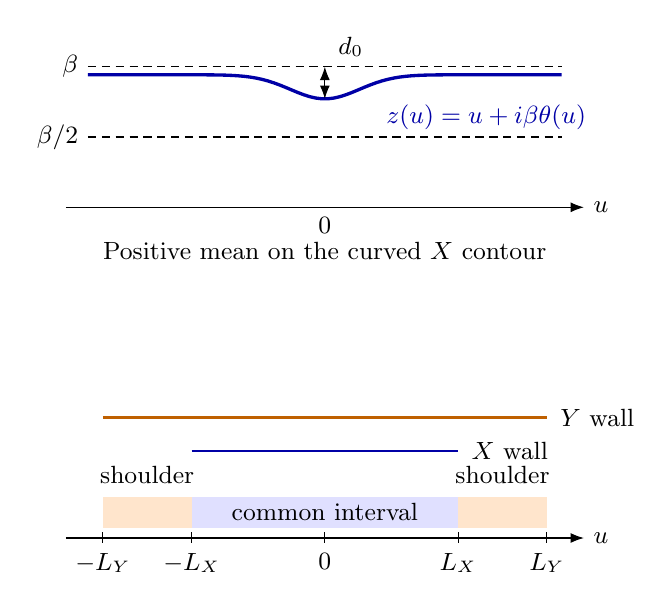
\begin{tikzpicture}[x=0.94cm,y=0.85cm,>=Latex,font=\small]
 \begin{scope}
  \draw[->] (-3.5,0)--(3.5,0) node[right] {$u$};
  \draw[densely dashed] (-3.2,1.05)--(3.2,1.05);
  \draw[densely dashed] (-3.2,2.1)--(3.2,2.1);
  \node[left] at (-3.2,1.05) {$\beta/2$};
  \node[left] at (-3.2,2.1) {$\beta$};
  \draw[blue!65!black,very thick,domain=-3.2:3.2,samples=80]
      plot (\x,{1.98-0.36*exp(-2.3*\x*\x)});
  \node[blue!65!black,anchor=west] at (0.7,1.35) {$z(u)=u+i\beta\theta(u)$};
  \node[below] at (0,0) {$0$};
  \draw[<->] (0,1.62)--(0,2.1);
  \node[above,anchor=south west] at (0.05,2.1) {$d_0$};
  \node at (0,-0.65) {Positive mean on the curved $X$ contour};
 \end{scope}
 \begin{scope}[yshift=-4.2cm]
  \fill[orange!20] (-3,0.15) rectangle (-1.8,0.62);
  \fill[blue!12] (-1.8,0.15) rectangle (1.8,0.62);
  \fill[orange!20] (1.8,0.15) rectangle (3,0.62);
  \draw[->] (-3.5,0)--(3.5,0) node[right] {$u$};
  \foreach \x/\lab in {-3/-L_Y,-1.8/-L_X,0/0,1.8/L_X,3/L_Y} {
    \draw (\x,-0.07)--(\x,0.09);
    \node[below] at (\x,-0.08) {$\lab$};
  }
  \node at (0,0.385) {common interval};
  \node[above] at (-2.4,0.67) {shoulder};
  \node[above] at (2.4,0.67) {shoulder};
  \draw[thick,blue!65!black] (-1.8,1.3)--(1.8,1.3);
  \draw[thick,orange!75!black] (-3,1.8)--(3,1.8);
  \node[right] at (1.85,1.3) {$X$ wall};
  \node[right] at (3.05,1.8) {$Y$ wall};
 \end{scope}
\end{tikzpicture}
\caption{Two distinct geometries in the magnetic estimate. Above, the
main $X$ contour carries a positive mean; the central distance $d_0$
can become small when almost all $X$ sites are upper sites. Below,
the particle numbers set different logarithmic wall lengths. The sharp
trial field treats the common interval and its two shoulders separately.
The curves and lengths are schematic.}
\label{fig:magnetic-geometry}
\end{figure}


The probability density and its transform are
\[
 \rho(w)=\frac{\sinh(2\gamma w)}
 {\sqrt3\,\beta\sinh(3\gamma w)},\qquad
 \widehat\rho(k)=\frac1{c_*(k)},\qquad
 c_*(k)=2\cosh(\beta k)-1 .
\]
The apparent singularity at \(w=0\) is removable.
Let \(\mathfrak R\) be its analytic primitive on
\(|\Im w|<\beta\), normalized by \(\mathfrak R(0)=0\).
We construct the contour as a level set of the imaginary primitive.
Its uniform Lipschitz bound will suffice for real-energy coercivity.
When \(t\) tends to one, the finer central estimates below will also
control smoothing and the particle coordinates used for fluctuations.

\begin{lemma}[Positive-density contour and its uniform regularity]
\label{lem:06-magnetic-curve}
For \(1/2\le t<1\), there is a unique real-analytic even function
\(\theta:\R\to[1/2,1)\) satisfying, with
\(z(u)=u+i\beta\theta(u)\),
\begin{equation}
 \Im\bigl[(1-t)\mathfrak R(z(u))
             +t\mathfrak R(z(u)-i\beta)\bigr]=0.
 \label{eq:06-curve}
\end{equation}
For \(t=1\), take \(\theta=1\) and \(\nu_X=\rho\).  For \(t<1\), define
\begin{equation}
 \nu_X(u)=
 [(1-t)\rho(z(u))+t\rho(z(u)-i\beta)]\,z'(u).
 \label{eq:06-density}
\end{equation}
In every case \(\nu_X\) is real, positive, even, and has integral one.
The graphs \(z\) are uniformly Lipschitz for \(t\in[1/2,1]\).
There is a unique \(\theta_\infty\in[1/2,1]\) satisfying
\begin{equation}
 (1-t)\sin(\gamma\beta\theta_\infty)
 +t\sin(\gamma\beta(\theta_\infty-1))=0,
 \label{eq:06-limit-height}
\end{equation}
and \(\theta(u)-\theta_\infty\) tends to zero exponentially with every
fixed-order derivative, uniformly in \(t\).
Outside any fixed neighborhood of zero, the curves and the
correspondingly rescaled tail densities
\(e^{\gamma|u|}\nu_X(u)\) have uniform analytic bounds, and
\(\nu_X(u)\asymp e^{-\gamma|u|}\).

More precisely, put \(r=1-t>0\),
\(\Delta(u)=\beta(1-\theta(u))\), and \(d_0=\Delta(0)\).
As \(r\downarrow0\),
\begin{equation}
 d_0\asymp r\log(1/r),\qquad
 \sup_u\left(
 |z(u)-(u+i\beta)|+|z'(u)-1|
 +\left|\frac{\nu_X(u)}{\rho(u)}-1\right|\right)=o(1).
 \label{eq:06-center-regularity}
\end{equation}
On a fixed small interval around zero, for each integer \(j\ge1\),
\[
 (|u|+d_0)^j
 \left(
 |\partial_u^j(z'(u)-1)|
 +|\partial_u^j(\nu_X(u)-\rho(u))|
 \right)=o(1)
\]
uniformly in \(u\).
The odd increasing change of coordinates \(b_X\) defined by
\[
 \int_0^{b_X(u)}\rho(v)\,dv=\int_0^u\nu_X(v)\,dv
\]
has \(b_X(u)-u=o(1)\) and \(b_X'(u)=1+o(1)\) uniformly as
\(t\uparrow1\), with the same scaled estimates for positive-order
derivatives of \(b_X'-1\).
\end{lemma}

\begin{proof}
The choice at \(t=1\) has all the asserted positivity and mass properties.
We construct the contour for \(t<1\), then prove the uniform estimates
as \(t\uparrow1\).
First \(\Re\rho(w)>0\) throughout \(|\Im w|<\beta\).
To verify the sign away from the removable zero, write
\(\gamma w=x+iy\), so \(|y|<\pi/3\).
The numerator of the real part, up to a positive factor, is
\[
 \cosh(5x)\cos y-\cosh x\cos(5y).
\]
Here \(\cos y>0\) and
\(\cos y-\cos(5y)=2\sin(3y)\sin(2y)\ge0\);
strict positivity follows except at the removable case \(x=y=0\),
where \(\rho(0)>0\).

Set
\(\Phi_t(u,y)=\Im[(1-t)\mathfrak R(u+iy)
 +t\mathfrak R(u+i(y-\beta))]\).
Its derivative in \(y\) is strictly positive for \(0<y<\beta\).
By conjugation symmetry,
\(\Phi_t(u,\beta/2)\le0\) for \(t\ge1/2\).
At \(y\uparrow\beta\), its second summand tends to zero and the
first is strictly positive, possibly infinite at \(u=0\).
The intermediate value theorem and strict monotonicity give the
unique root.  The analytic implicit-function theorem gives
real analyticity, and symmetry in \(u\) gives evenness.

For positivity of \(\nu_X\), write
\(A=(1-t)\rho(z)+t\rho(z-i\beta)=a+ib\), with \(a>0\).
Differentiating \(\Phi_t(u,\beta\theta(u))=0\) gives
\(\beta\theta'=-b/a\), and hence
\[
 \nu_X=A(1+i\beta\theta')=\frac{|A|^2}{a}>0.
\]
Evenness follows from conjugation symmetry.
Moving each translated density contour within its pole-free strip
shows \(\int\nu_X=1\).  Equivalently the primitive in
\eqref{eq:06-curve} tends to \(1/2\) and \(-1/2\) at its two ends.

The exponential expansion of \(\rho\) at either end begins with a
positive multiple of \(e^{-\gamma|u|}\).
Substitution into the imaginary primitive equation, divided by
this leading term, gives \eqref{eq:06-limit-height}.
Its derivative with respect to \(\theta_\infty\) is bounded below
uniformly, since both relevant cosine arguments lie in
\([-\pi/3,\pi/3]\).  The analytic implicit-function theorem applied
to the exponentially small remainder proves the uniform tail
statements, including fixed-order derivatives.  On compact
\(t\)-subintervals below one, the same conclusions in the remaining
bounded \(u\)-region follow by compactness and the strict derivative
in \(y\).

It remains to examine the possible central degeneration as
\(r=1-t\downarrow0\).  At \(w=i\beta\), the density has a simple
pole with negative imaginary residue, explicitly
\(-i/(6\beta\gamma)\).
On a sufficiently small fixed interval in \(u\), the defining
equation therefore compares
\[
 -(1-r)\Im\mathfrak R(u-i\Delta)\asymp\Delta
\]
with
\[
 r\Im\mathfrak R(u+i\beta-i\Delta)
 \asymp r\left(1+\log^+\frac1{|u|+\Delta}\right).
\]
At \(u=0\) this gives \(d_0\asymp r\log(1/r)\).
The same estimates, separating \(|u|\le d_0\) and \(|u|>d_0\),
give \(|u|+\Delta(u)\asymp |u|+d_0\).

To obtain uniform derivative bounds, write the defining equation as
\[
 F_r(u,\Delta)
 =r\Im\mathfrak R(u+i\beta-i\Delta)
  +(1-r)\Im\mathfrak R(u-i\Delta)=0.
\]
The regular function vanishes identically when \(\Delta=0\), and its
Taylor expansion on this fixed central interval is
\[
 \Im\mathfrak R(u-i\Delta)=-\Delta\rho(u)+O(\Delta^3).
\]
Thus its \(u\)-derivative is \(O(\Delta)\), whereas its
\(\Delta\)-derivative is \(-\rho(u)+O(\Delta^2)\).
Either first derivative of the pole summand, including its coefficient,
is bounded by
\[
 O\!\left(\frac{r}{|u|+d_0}\right)
 =O\!\left(\frac1{\log(1/r)}\right)=o(1).
\]
Since \(\rho\) is bounded below here and \(\Delta=o(1)\), it follows that
\[
 |\partial_\Delta F_r|\ge c_3>0,\qquad
 |\partial_u F_r|
 \le C\left(\Delta+\frac{r}{|u|+d_0}\right)=o(1).
\]
In particular \(\Delta'=-\partial_u F_r/\partial_\Delta F_r=o(1)\).
For higher derivatives, extend each imaginary part analytically using
the two conjugate analytic terms.  Around a real solution at \(u_0\),
take complex discs in \(u,\Delta\) of radii
\(c_2(|u_0|+d_0)\).  The pole remains outside these discs when
\(c_2\) is sufficiently small.  The \(\Delta\)-derivative remains
bounded away from zero, while varying \(u\) with \(\Delta=\Delta(u_0)\)
changes \(F_r\) by \(o(1)(|u_0|+d_0)\), by the same estimates.
The analytic implicit root therefore extends to a disc of comparable
radius with oscillation \(o(1)(|u_0|+d_0)\).  Cauchy's estimates give
\(z'-1=o(1)\) and the stated scaled higher-derivative bounds.
The formula for \(\nu_X\) gives the same estimates for
\(\nu_X-\rho\).  In this central region \(\rho\) is bounded below;
off it the uniform tail expansion supplies the relative estimate
in \eqref{eq:06-center-regularity}.  These statements prove, in
particular, uniform Lipschitzness and uniform comparison
\(\nu_X\asymp\rho\) throughout the parameter interval.

Finally the cumulative distributions are strictly increasing and
have identical total mass.  Analytic inversion on bounded
intervals, and inversion of their normalized exponential tails,
show that their matching map \(b_X\) is odd and obeys the claimed
uniform displacement and derivative bounds.  Differentiating
\(\rho(b_X)b_X'=\nu_X\) on the same analytic discs gives the scaled
higher-derivative estimates.
\end{proof}

\subsection{Exact centering of the ordinary and marked factors}

Label the six species by \(I=(\sigma,J)\), where \(J=0,F,P\)
denotes main, far singleton, or far double, and let
\(w_I=1,1,2\), respectively.  On each species use the real coordinate
\(u\) as its integration coordinate; only the main \(X\) species
follows the curved graph \(z(u)\).
Let \(H\) be minus the sign-normalized particle--particle logarithm,
and \(V\) the sign-normalized ordinary site--particle logarithm,
with the following logarithm convention. Reduce each angle to
$[0,2\pi)$ and use linear combinations of
\[
 K_\vartheta(u)=-\log\!\left[2\left(\sin(\vartheta/2)\cosh(u/2)
       -i\cos(\vartheta/2)\sinh(u/2)\right)\right],\quad
 K_0(u)=-\log|2\sinh(u/2)|.
\]
The particle factors determine the exponents in $H$; the negative
site--particle exponents determine $V$. Reverse cross entries by
transposing and reflecting the argument. Fourier transforms use
$\widehat f(k)=\int e^{-iku}f(u)\,du$ and inverse measure $dk/(2\pi)$.
At nonzero frequency,
\[
 \widehat K_\vartheta(k)=\frac{\pi e^{(\pi-\vartheta)k}}
                              {k\sinh(\pi k)},\qquad
 \widehat K_0(k)=\frac{\pi\cosh(\pi k)}{k\sinh(\pi k)}.
\]
The transforms follow by differentiating twice and taking the double
pole residue; symmetric averaging gives the angle-zero case.
Affine ambiguities are fixed by the real tails $-|u|/2+O(e^{-|u|})$
and the odd imaginary tails
$(\pi-\vartheta)\operatorname{sign}(u)/2$. The forms extend
bilinearly to complex measures.

For the curved main self interaction, retain the horizontal
logarithm and add the continuous logarithm of the ratio of its
curved and horizontal factors.  In particular the two vanishing
sinh factors are divided before this correction is taken.
Choose the logarithm that is zero before contour deformation.
This prescription fixes the diagonal continuation and gives kernels
conjugated by simultaneous negation of both real coordinates.
Constant signs depend only on the species counts.

Put
\[
 \mu_X=s\nu_X(u)\,du,\qquad
 \mu_Y=b\rho(u)\,du,\qquad \mu_I=0\quad(I\ {\rm far}),
\]
and write \(\mathfrak t_I^{\,a}\) for the particle logarithm of the
single-mark factor
\(\prod_vP_{-4\sigma_v}(v-a)/P_{\sigma_v}(v-a)\).

\begin{lemma}[Magnetic mean identities]
\label{lem:06-magnetic-mean}
The ordinary one-body logarithm is \(H\mu\).
Multiplying the ordinary site-pair factors by
\(\exp((\mu,H\mu)/2)\) gives, up to a constant sign,
\begin{equation}
 C_*^n\prod_{\substack{i<j\\i,j\in X\cup Y}}H_*(a_i-a_j)^2,
 \qquad
 C_*=\frac{(1+d)\gamma}{4d\cos(\beta/2)}.
 \label{eq:06-ordinary-mean}
\end{equation}
For each marked log \(a\), its site factors in \(\mathcal T\),
multiplied by \(\exp((\mathfrak t^{\,a},\mu))\), give, again up to
a constant sign,
\begin{equation}
 \prod_{i\in X\cup Y}H_*(a_i-a)^2.
 \label{eq:06-marked-mean}
\end{equation}
On either main contour the real part of
\(\mathfrak t_I^{\,a}\), together with its first derivative, decays
exponentially at infinity.  Its imaginary part tends exponentially
to
\(\sigma_I(3\beta/2)\operatorname{sign}u\).
The logarithm is regular with uniformly bounded first derivative
at the center.  On far species one has an exponentially decreasing
upper bound for its real part; zeros of its numerator are allowed.
\end{lemma}

\begin{proof}
We justify the contour continuations in the Fourier mean
identities, since the \(X\) site measure now has two different
heights.  For a test on the \(X\) main contour, slide separately the
two translated \(\rho\) contours to a horizontal line through the
test point, keeping that line at distance strictly less than
\(\beta\) from the relevant site height.  For the diagonal
logarithm, split the contour at the test point and deform its two
halves with this common endpoint.  Its logarithmic singularity is
integrable, and the chosen continuous branch crosses no cut.
For any other test species use a fixed admissible horizontal
height between \(\beta/2\) and \(\beta\).

No additional singularity is met in these slides.
The signed same-group separation of a far elementary particle from
a main contour or its associated horizontal site line has absolute
value strictly between \(2\beta\) and \(5\beta\).
The cross separation, with the \(X\) coordinate first, is positive
and less than \(6\beta\).
All these bounds follow directly from the listed contours.
They also hold for the slides used in a second pairing with a
site's translated density.  A same-group \(V\) is always slid
within distance \(\beta\) of its site.  Coincident site--main
heights in a cross \(V\) are regular.

On horizontal contours Fourier transforms use
\(\widehat f(k)=\int e^{-iku}f(u)\,du\); put \(x=\beta k\).
The self-main entry has transform
\[
 \widehat H_{\rm self}(k)
 =\frac{2\pi c_*(k)\cosh(3x)}{k\sinh(\pi k)}.
\]
For a same-group far elementary particle at signed height
separation \(j\beta\), replace the numerator
\(c_*\cosh(3x)\) by
\[
 c_*\cosh(x)e^{(4\operatorname{sign}j-j)x}.
\]
For a cross elementary pair at separation \(d\beta>0\), replace it
by \(c_*e^{(3-d)x}\), transposing by \(k\mapsto-k\) when the row
and column are reversed.
Convolution with each translated \(\rho\) cancels \(c_*\);
the translation multiplier adjusts the height from its main
contour to its site.  These are exactly the transforms of the
corresponding \(V\) entries.  This proves the one-body identity.

Pair once more with the translated density of a second site.
For a horizontal same-group pair the symbol of
\(\log B_s+\rho*H_{\rm self}*\rho\), divided by
\(2\pi/(k\sinh(\pi k))\), is
\[
 -\cosh(2x)-\cosh x+\frac{\cosh(3x)}{c_*(k)}
 =-2\cosh x+\cosh(4x)-\sinh(4x)\tanh(3x/2).
\]
The expression on the right is the symbol of \(\log H_*^2\) in the
same normalization: factor \(H_*\) and use
\(\widehat{\log|\tanh(\gamma u/2)|}(k)
=-\pi\tanh(3\beta k/2)/k\).
This is the horizontal centering calculation of
\cite[Lemma~3.1]{Electric}; the contour slides above extend it to
the two site heights here.  In the cross case one may first compute
at positive main--main separation and undo that shift in the
transforms.  The cancellation needed there is
\[
 \frac{\sinh(3x)}{c_*(k)}=\sinh(2x)+\sinh x.
\]
Endpoint identities at a height difference \(\beta\) follow by
moving the heights slightly inward and taking the regular limit.
The half self term for each site is fixed by the same-group identity
at zero.  With the affine terms fixed by the tails as below, this gives
\[
 \exp\!\left(\tfrac12(\rho*H_{\rm self}*\rho)(0)\right)
 =\frac{H_*(0)}{\sqrt{B_s(0)}}
 =\frac{\gamma(1+d)}{4d\cos(\beta/2)}=C_*.
\]
Here \(H_*(0)=\gamma(1+d)\) and
\(\sqrt{B_s(0)}=4\sin\beta\sin(3\beta/2)=4d\cos(\beta/2)\),
with the positive square root.  There is one such factor per ordinary
site, proving \eqref{eq:06-ordinary-mean} with its exact normalization.

For a single mark, slide the density in the same way.
After removing the ordinary-site to marked-site translation
multiplier, the combined log symbol, divided by
\(-\pi/(k\sinh(\pi k))\), is
\[
 e^{2\sigma x}+e^{\sigma x}
 +\frac{1-e^{3\sigma x}}{c_*(k)}
 =
 2\left(\cosh(2x)+\cosh x-\frac{\cosh(3x)}{c_*(k)}\right).
\]
The equality follows by multiplying by \(2\cosh x-1\).
This is exactly the symbol of \(\log H_*^2\), proving
\eqref{eq:06-marked-mean}.
These transform comparisons determine the second derivatives.
To fix the affine ambiguity, subtract the linear real tails:
the remaining real constants vanish by the exponential expansions
and the centered real offsets; a translated \(\rho\) has purely
imaginary first moment.  On horizontal contours the imaginary
parts are bounded and odd, so their affine ambiguity vanishes as
well.  Continuing the chosen logarithms fixes the stated signs.

Finally on a main contour the numerator angle of a marked particle
factor is reduced to \(4\) plus the relevant shift, in units of
\(\beta\), and the denominator angle is \(1\) or \(7\) plus that
shift.  These angles stay in the open interval \((0,8)\).
The log-sinh tail expansion therefore gives zero real limit,
exponential real decay with a derivative, and the imaginary
limits \(\sigma(3\beta/2)\operatorname{sign}u\).
The compact part remains uniformly regular because the main
angles stay away from zeros and \(z'\) is uniformly bounded by
Lemma \ref{lem:06-magnetic-curve}.
On far contours the denominator remains regular and the same
tail expansion bounds the log modulus above by \(Ce^{-c_2|u|}\).
A numerator zero only improves this upper bound.
\end{proof}

\subsection{Positivity of the real energy}

For a real vector of smooth rapidly decreasing densities
\(\xi=(\xi_I)\), assume weighted neutrality and define
\[
 \int_{\R}\sum_Iw_I\xi_I=0,\qquad
 d_\xi=\sum_Iw_I\xi_I,\qquad
 D(u)=\int_{-\infty}^u d_\xi(v)\,dv,\qquad
 B(\xi)=\tfrac12(\xi,\Re H\,\xi).
\]
Use the inhomogeneous negative Sobolev norm
\[
 \|\xi_I\|_{-1/2}^2
 =\int_{\R}(1+k^2)^{-1/2}|\widehat\xi_I(k)|^2
 \,\frac{dk}{2\pi}.
\]

\begin{theorem}[Uniform real-energy coercivity]
\label{thm:06-real-positivity}
For the magnetic contours there are constants \(0<c_2<C_2<\infty\)
such that
\begin{equation}
 c_2\left(\|D\|_2^2+\sum_I\|\xi_I\|_{-1/2}^2\right)
 \le B(\xi)\le
 C_2\left(\|D\|_2^2+\sum_I\|\xi_I\|_{-1/2}^2\right).
 \label{eq:06-real-positivity}
\end{equation}
They are uniform in \(t\in[1/2,1]\) and in all sufficiently small
positive far-contour parameters \(\varepsilon\).
The form extends to the completion in this norm.
\end{theorem}

\begin{proof}
We will sweep the curved \(X\) charge harmonically to the two edges
of the strip between heights \(\beta/2\) and \(\beta\).
The boundary energy and the remaining positive Green energy together
will control both the species norms and the weighted total primitive.

\par\smallskip\noindent\textbf{The horizontal boundary lines.}
Allow independent \(X\) main charges on the two boundary lines.
This gives a translation-invariant system with seven species.
At \(\varepsilon=0\), their elementary
height lists, in units of \(\beta/8\), are
\[
 (4),\quad(8),\quad(25),\quad(24,32),\quad
 (0),\quad(-28),\quad(-24,-32).
\]
The first four species belong to \(X\); the final three belong to
\(Y\).  Divide the real Fourier symbol by
\(\pi/(k\sinh(\pi k))\), and divide its \(IJ\) entry by
\(w_Iw_J\).  Expand the resulting matrix in
\(v=\cosh(\beta k/8)-1\).  Its constant matrix has every entry
equal to \(2\), and every coefficient of degree
\(1\le l\le32\) is strictly positive definite.
Here is a finite rational verification of this assertion.

The coefficient of \(v^l\) in \(\cosh(32\,\operatorname{arcosh}(1+v))\)
is
\[
 c_{32,l}=\frac{2^l}{(2l)!}
 \prod_{a=0}^{l-1}(32^2-a^2)>0.
\]
After division by this coefficient, define
\[
 h_l(j)=
 \prod_{a=0}^{l-1}\frac{i_j^2-a^2}{32^2-a^2},
 \qquad i_j=(j\bmod64)-32.
\]
For each pair of elementary heights, let \(j\) be their absolute
difference.  Average over the two species' height lists the
expression
\[
 2h_l(j)+h_l(j+16)+h_l(j-16)-h_l(j-8)-h_l(j+8)
\]
when they are in the same group, and
\[
 2\bigl(h_l(j)+h_l(j+16)-h_l(j+8)\bigr)
\]
when they are in opposite groups.  Denote the resulting symmetric
matrix by \(M_l\).
These formulas follow by summing the log-factor angles modulo
\(2\pi=8\beta\).  The elementary cosh coefficient formula follows
from
\((2v+v^2)y''+(1+v)y'=i_j^2y\).

For \(l\le12\), symmetric elimination gives successive pivots
strictly larger than the rational decimals in the following table:
\[
\begin{array}{c|rrrrrrr}
 l&1&2&3&4&5&6&7\\ \hline
 1&1&.7&.8&.27&.49&.59&.09\\
 2,3&1&1&1&.32&.8&1&.30\\
 4,5,6&1.7&1.65&1.48&.35&1.53&1.65&.45\\
 7,\ldots,12&1.9&1.88&1.74&.35&1.89&1.88&.48
\end{array}
\]
The entries are obtained using exact rational substitution in
\[
 m_{ij}^{(p)}
 =m_{ij}^{(p-1)}
 -\frac{m_{ip}^{(p-1)}m_{jp}^{(p-1)}}{m_{pp}^{(p-1)}},
 \qquad i,j>p,\qquad M_l=(m_{ij}^{(0)}).
\]
Thus all these matrices are positive definite.

For \(13\le l\le32\), each \(h_l(j)\) is nonnegative and
nonincreasing in \(l\): before a zero occurs, every additional
factor lies in \([0,1]\), and after that zero the product stays
zero.  Split the displayed averages into their positive and
negative parts, \(M_l=P_l-Q_l\).  A lower bound for its diagonal
is \(\operatorname{diag}(P_{32}-Q_{13})\), and an entrywise upper
bound for the absolute off-diagonal entries is
\[
 \max(P_{13}-Q_{32},\,Q_{13}-P_{32}).
\]
Weight column \(j\) relative to row \(i\) by \(v_j/v_i\), with
\(v=(1,1,1,2,1,1,1)\).
Subtracting the weighted off-diagonal row sums from the diagonal
lower bounds gives exactly
\[
\begin{split}
 (&539085539017/288991072832,\ 
 153103458093/288991072832,\ 
 6754920483/37289170688,\\
 &2413205499/288991072832,\ 
 8798842243/4515485513,\\
 &496150561213/288991072832,\ 
 32952783649/1155964291328).
\end{split}
\]
All seven numbers are positive.  Weighted strict diagonal
dominance of the symmetric \(M_l\) proves positive definiteness
for every remaining degree.

At small frequencies the constant coefficient supplies the
rank-one \(k^{-2}\) term for the weighted total density, and the
strictly positive first coefficient supplies a uniformly positive
bounded term on all species.  At large frequencies the top
coefficient supplies a positive multiple of \(1/|k|\), since
\(\pi=4\beta\).  The intervening frequencies are controlled by
continuity and positivity.  The real tail
\(-w_Iw_J|u-v|\) contributes exactly \(\|D\|_2^2\) to \(B\).
These observations prove the two-sided norm estimate on the
seven boundary-line species at \(\varepsilon=0\).

\par\smallskip\noindent\textbf{Uniform movement of the far double.}
The estimate continues uniformly to sufficiently small
\(\varepsilon>0\).  At small frequencies use the strict positive
quadratic coefficient, and on compact frequency intervals use
continuity.  To check uniformity at infinite frequency, divide
the normalized symbol further by \(\cosh(4\beta k)\).
For \(0\le\varepsilon<1/16\) it has the form
\[
 \operatorname{diag}(2,2,2,\tfrac12,2,2,\tfrac12)
 +q_\varepsilon(k)(E_{24}+E_{42})
 +O(e^{-c_3|k|}),\qquad
 q_\varepsilon(k)=
 \frac{\cosh((4-\varepsilon)\beta k)}{2\cosh(4\beta k)}.
\]
Here \(E_{ij}\) is the elementary matrix, and the error is uniform
in \(\varepsilon\): after collecting the elementary factors of
each double, all other contributing angles stay a fixed distance
from zero modulo \(8\beta\).  In particular the potentially small
angles in the \(X\)-double/\(Y\)-double entry cancel with total
coefficient \(2-4+2=0\), for every \(\varepsilon\).
The exceptional pair couples the \(X\) main line of height
\(\beta\) to the \(X\) double, and \(0\le q_\varepsilon\le1/2\).
The only nontrivial \(2\) by \(2\) block is
\(\left(\begin{smallmatrix}2&q\\q&1/2\end{smallmatrix}\right)\);
its least eigenvalue is at least
\((5-\sqrt{13})/4>0\).
This proves uniform coercivity also in every joint limit
\(\varepsilon\downarrow0\), \(|k|\to\infty\).

\par\smallskip\noindent\textbf{Harmonic sweeping to the boundary.}
We now pass from the two boundary lines to the graph.
Let \(\mathcal S=\{z:\beta/2<\Im z<\beta\}\), and balayage the
real charge on the graph harmonically to the two edges of
\(\mathcal S\).  Leave all other species unchanged, and denote the
resulting seven-species charge by \(\widetilde\xi\).
All interactions are harmonic in this strip, in either variable
away from the source, and have at most linear growth.
The only interior source in a graph self interaction is
\[
 -2\log\left|2\sinh\frac{z-z'}2\right|,
\]
whose logarithmic singularity is \(-2\log|z-z'|\).
Let \(G_{\mathcal S}\) be the Dirichlet Green kernel of
\(-\Delta\), with singularity
\(-(2\pi)^{-1}\log|z-z'|\), and put
\[
 \mathcal G(\xi_X)=
 \iint G_{\mathcal S}(z(u),z(v))\,\xi_X(u)\xi_X(v)\,du\,dv.
\]
Harmonic interpolation first in one variable and then in the other
therefore gives the exact identity
\begin{equation}
 B(\xi)=B_{\partial\mathcal S}(\widetilde\xi)
              +2\pi\mathcal G(\xi_X).
 \label{eq:06-balayage}
\end{equation}
The coefficient \(2\pi\) includes the factor \(1/2\) in the
definition of \(B\).
The Green energy is nonnegative for signed real charges: by
Dirichlet inversion and integration by parts it is the squared
dual norm of the charge acting on traces of zero-boundary
functions with gradient \(L^2\)-norm at most one.
Harmonic measures in the strip decay exponentially; their Fourier
kernels are ratios of the form
\(\sinh(yk)/\sinh(\beta k/2)\).
These facts justify the interpolations for rapidly decreasing
densities and then by completion.

\par\smallskip\noindent\textbf{Uniform control as the graph approaches an edge.}
For clarity, we verify that \eqref{eq:06-balayage} gives exactly
the claimed norm, even when the graph approaches the upper edge.
The Sobolev trace principle underlies this comparison
\cite[Theorem~1.I]{Gagliardo1957Trace}; we give the strip construction
to retain uniform constants as the graph approaches an edge.
The trace map \(H^1(\R^2)\to H^{1/2}(\R)\) on the graph and a right
inverse both have bounds depending only on its uniform Lipschitz
constant.  Flatten the graph by a uniformly bilipschitz map.
On a horizontal line, the trace bound follows by transverse
Fourier Cauchy--Schwarz, and a right inverse extends a mode \(k\)
by \(e^{-\sqrt{1+k^2}|y|}\).
Reflection across the strip edges with a cutoff gives the same
trace bound for strip functions.
Harmonic extension from the two boundaries is bounded
\(H^{1/2}\to H^1\); this follows either from the displayed
Fourier kernels or the Dirichlet principle together with the
fixed strip width.

Duality now bounds the two projected charges' \(H^{-1/2}\) norms
by the graph charge's norm.  It also bounds the Green energy above
by that squared norm, since zero-boundary strip functions have
their full \(H^1\) norm controlled by their gradient.
Conversely, extend an arbitrary \(H^{1/2}\) test on the graph to
the plane, restrict it to the strip, and decompose it into its
harmonic boundary extension and a zero-boundary remainder.
Pairing these two terms with the charge gives
\[
 \|\xi_X\|_{-1/2}^2
 \le C_3\left(
 \|\widetilde\xi_{X,\beta/2}\|_{-1/2}^2+
 \|\widetilde\xi_{X,\beta}\|_{-1/2}^2+
 \mathcal G(\xi_X)\right).
\]
Thus the Sobolev parts of the norms are equivalent in both
directions, with the Green term included.

It remains to compare primitives of the weighted total densities.
Let \(\widetilde D\) be the primitive after projection.
For a smooth compactly supported function \(b\), pair the
horizontal marginal of the difference between graph charge and
projected charge with \(b\).  This pairing equals that of the
graph charge with \(b(u)\) minus the harmonic extension of the
same boundary value \(b\) on both edges.
The latter difference has zero boundary values and gradient norm
at most \(C_4\|b'\|_2\): compare the harmonic extension to the
constant-in-height function \(b(u)\) by the Dirichlet principle.
Green-energy duality, followed by integration by parts in \(u\),
therefore yields
\[
 \|D-\widetilde D\|_2^2\le C_5\mathcal G(\xi_X).
\]
Together with \eqref{eq:06-balayage}, the boundary-line coercivity,
and the Sobolev norm comparisons, this proves both inequalities
in \eqref{eq:06-real-positivity}.
All constants depend only on the fixed strip width and uniform
Lipschitz bounds, so remain uniform as the graph reaches an edge,
including the case \(t=1\).
\end{proof}

\section{Magnetic trial actions with unequal walls}
\label{sec:07_magnetic_analysis-trials}

The next estimates retain a positive part of the real energy while gaining
$2L_X$ from the common interval and controlling the activities on the two
shoulders. We first define the trial action, then separate its smoothing,
common-interval, and shoulder estimates. The resulting bounds will be
implemented in the actual particle integral in the next section.

\subsection{Explicit particles and the trial action}

Retain the magnetic contours, their elementary multiplicities \(w_I\),
and the real-energy form \(B\) of the preceding section. A double label
always represents the sum of its two elementary constituents when a kernel
is computed. Write $s_X=s$, $s_Y=b$, $\bar\nu_X=\nu_X$ and
$\bar\nu_Y=\rho$ for their sizes and positive unit-mass mean densities.
The two main labels are \(X,Y\); the subscript \(n\)
means the pair of main labels. Throughout this section,
\[
 \beta=\frac\pi4,\qquad \gamma=\frac\pi{3\beta}=\frac43,
 \qquad \kappa=(3\beta)^2,\qquad
 p=(3-\theta_\infty)\beta,\qquad L=L_Y.
\]
The parameter \(p\) in the kernel formulas is distinct from a marked port.
We assume \(c_1L\le L_X\le L_Y=L\), with \(c_1>0\) fixed.
Constants can depend on \(c_1\). An error \(o(L)\), or \(o(1)B(x)\),
is uniform over the stated frozen configurations after all smoothing,
localization, and projection parameters have been fixed. When counts are
restricted to a fixed power of \(L\), uniformity includes the positions
and counts in that restriction. Errors denoted \(o_\varepsilon(1)L\)
have a coefficient tending to zero as \(\varepsilon\downarrow0\), with
\(h=\varepsilon^{K_2}\) as specified below; they are different from the
large-\(L\) errors.

Split main particles at their respective walls \([-L_g,L_g]\).
Put the particles outside their own walls, together with every far-label
particle, into the explicit configuration \(\zeta\). Its total number is
\(n_e\), with elementary multiplicities included whenever a group total
is tested. The interior density \(\alpha_g\) has mass \(m'_g\), obtained
by subtracting these explicit multiplicities from \(s-M,b+M\).
Here \(M\) remains an integer. We use the following explicit regularization. Fix a small $h>0$.
Let $\psi=\psi^{(h)}$ be the even positive convolution probability
whose Fourier transform averages
$\cosh((\pi-hv)k)/\cosh(\pi k)$ over $0<v<1$, with probability
density proportional to $e^{-1/\sqrt v}$. Before averaging its
real density is
\[
 \frac{\cosh(u/2)\sin(hv/2)}
 {2\pi(\sinh^2(u/2)+\sin^2(hv/2))}.
\]
Hence $\psi\le C/h$, its tails are at most $Ch e^{-|u|/2}$ for
$|u|\ge1$, and $\int u^2\psi(u)\,du\le Ch$. Its Fourier
transform has upper and lower stretched-exponential bounds of the
form $C e^{-c(h|k|)^{1/3}}$ and $c e^{-C(h|k|)^{1/3}}$.
Put $S_0(u)=-2\log|2\sinh(u/2)|$. Then
$S_0\ge S_0*\psi\ge S_0*\psi*\psi$ by the preceding Fourier
formula with the real tails fixed. Choose an even Gevrey cutoff
$\chi$, equal to one on $[-1/2,1/2]$, zero outside $[-1,1]$, and
between zero and one. On like-main interior/explicit entries set
\[
 R_h(u)=\chi(u)(S_0-S_0*\psi)(u)\ge0,\qquad
 \widetilde H_{ne}=H_{ne}-R_h,
\]
with $R_h=0$ on other entries. We also write $R$ for this kernel
when no operator complement is involved. This cutoff uses the
horizontal difference, including on the curved contour. Define
\[
 \mathcal E(\alpha,\zeta)
 =\tfrac12(\alpha-\mu,H_{nn}(\alpha-\mu))
   +(\alpha-\mu,\widetilde H_{ne}\zeta)
   +\tfrac12(\zeta,H\zeta)_{\rm off}.
\]
The last expression omits each individual explicit self interaction;
near empirical diagonals will instead use smooth reference compensation. Put
\[
 x=\operatorname{Re}\alpha-\mu+\psi*\zeta,\qquad
 z=\operatorname{Im}\alpha,\qquad
 D'=\sum_Iw_Ix_I,\qquad D_z'=\sum_Iw_Iz_I.
\]
The primitives vanish at infinity, and each main component of \(z\) has
integral zero. To distinguish a contour from a density, write
\(\mathfrak z_I(u)\) for its complex parametrization; thus
\(\mathfrak z_X(u)=u+i\beta\theta(u)\) on main \(X\).
Let \(\mathfrak t_I\) be the sum of the particle logarithms from the two
marked anomalies. The trial action is
\[
 \mathcal D(\alpha,\zeta)
 =\mathcal E(\alpha,\zeta)
   -(\mathfrak t_n,\alpha-\mu)-(\mathfrak t,\zeta).
\]
A purely imaginary constant depending only on the species counts never
affects a bound on its real part.

\subsection{Reference measure and sector normalization}\label{sec:reference-law}

The comparison law has two independent labels, denoted $X,Y$. For an
integer $n\ge0$, its unnormalized measure on $[0,\pi]^n$ is
\[
 \frac1{n!}\prod_{i=1}^n\frac{2\sin t_i\,dt_i}{2\pi}
       \prod_{i<j}|2(\cos t_i-\cos t_j)|^2.
\]
Under $x=\cos t$ this is the Legendre orthogonal-polynomial ensemble.
Andr\'eief's determinant integration identity gives its mass
\cite[equation~(1.3)]{TracyWidom1998}
\begin{equation}\label{eq:reference-normalization}
 J_n=\prod_{i=0}^{n-1}
 \frac{2\cdot16^i(i!)^4}{\pi(2i+1)((2i)!)^2}
 =\exp\{-\tfrac14\log(n+1)+O(1)\},\qquad J_0=1.
\end{equation}
We write $\mathbb E_0$ only for the probability expectation, divided
by $J_{N_X}J_{N_Y}$. Neither of these factors is part of the
observable.

On each label, let $r\in[-A_g,A_g]$ be a real reference parameter
and let $t_g(r)$ be an increasing probability coordinate taking values
in $[0,\pi]$, with density $\lambda_g(r)=t'_g(r)/\pi$.
The corresponding point on the main contour is denoted by $Z_g(r)$.
We will specify this parametrization, including its endpoint caps, in
Section~\ref{sec:07_magnetic_analysis-fluctuations}. With $X_{N_g}$
the empirical counting measure in the reference parameter, put
\[
 q_g=X_{N_g}-N_g\lambda_g(r)\,dr,\qquad Q_g'=q_g,
 \qquad Q_g(-A_g)=Q_g(A_g)=0.
\]
The reference kernel is block diagonal, with each diagonal block
\[
 H_{\rm ref}(t,t')=-2\log|2(\cos t-\cos t')|.
\]
Its mean against $dt/\pi$ is zero. The Hilbert space $\mathcal X$
is the completion of smooth Dirichlet primitives for the form
\[
 h_0(Q,Q)=(Q',H_{\rm ref}Q')
    =\pi^2\sum_{g,n\ge1}n|b_{g,n}|^2,
 \qquad Q_g(t)=\sum_{n\ge1}b_{g,n}\sin(nt).
\]
Real symmetric forms extend bilinearly to complex arguments; norms
and adjoints always use the Hermitian convention. An empirical
primitive need not have finite $h_0$ energy. We evaluate its quadratic
cost only after subtracting the reference singularity, so that the
remaining kernel is smooth, including its diagonal. No subtraction of
two infinite self energies is involved.

Let $p_g$ be the pushforward of $\lambda_g(r)\,dr$ to the horizontal
coordinate of the $g$ wall, and write $p_L=(p_X,p_Y)$. For this
sector take $N_g=m'_g$, restricted to nonnegative integer counts.
Inserting $m'p_L+q$ into the trial action always means pushing $q$
to the same horizontal coordinates. The two interior empirical
measures are denoted by $X_{\rm int}=(X_{N_X},X_{N_Y})$; their
pushforward is likewise understood in pairings with the trial kernels.

We now compute the factor produced by changing to this reference law.
Put $a_*=2\cos(\beta/2)=d/c$. On a main label the local particle
factor and the reference pair factor have the respective expansions
\[
\begin{aligned}
 E_s(Z_g(r)-Z_g(r'))
   &=a_*^2Z'_g(r)^2(r-r')^2(1+o(1)),\\
 |2(\cos t_g(r)-\cos t_g(r'))|^2
   &=\bigl(2\sin t_g(r)t'_g(r)\bigr)^2(r-r')^2(1+o(1)).
\end{aligned}
\]
Consequently the smooth-diagonal compensation contributes
\[
 \exp\!\left(\frac{(H-H_{\rm ref})_{gg}(r,r)}2\right)
 =\frac{2\sin t_g(r)t'_g(r)}{a_*Z'_g(r)}.
\]
Here $H$ is composed with the contour parametrization, and the branch
is continued from the straight contour; endpoint values are taken by
continuity. Multiplication by $dZ_g(r)/(2\pi)$ cancels $Z'_g(r)$
and leaves $a_*^{-1}$ times the reference one-particle measure
$2\sin t_g\,dt_g/(2\pi)$.

The finite identity and ordinary mean extraction contribute
$((2d)C_*)^n$, where $n=N-2$ is the total elementary particle degree.
Since
\[
 \frac{(2d)C_*}{a_*}=\frac\gamma2,
 \qquad
 N_X+N_Y=n-\sum_{v\in\zeta}w_{I(v)},
\]
extracting $(\gamma/2)^n$ leaves $a_*^{w_I}$ for each explicit
particle of species $I$. Thus a singleton retains activity $d/c$,
and a double retains $4c^2(d/c)^2$. The magnetic mean identities
supply all ordinary and marked site-pair factors. Restoring the
missing marked--marked factor and replacing $n$ by $N$ in the
extracted power changes the result only by a uniformly bounded
factor, because the allowed marked log differences are $0,\pm i\beta$
and $H_*$ is nonzero there.

After extracting $(\gamma/2)^N\prod_{i<j}H_*(a_i-a_j)^2$, the
remaining sector is therefore an unnormalized reference integral
with integrand
\[
 A\exp\!\left(-\mathcal D(m'p_L+q,\zeta)
                       +\tfrac12H_{\rm ref}[q,q]\right),
 \qquad A=\exp(-(X_{\rm int},R\zeta)).
\]
The difference in the exponent uses smooth-diagonal compensation on
both labels, as above. Including the explicit integration measures,
the remaining prefactor is bounded in modulus by
\[
 C\prod_{v\in\zeta}
 \left(\frac{|d\mathfrak z_{I(v)}(v)|}{2\pi}
 (d/c)^{w_{I(v)}} a_{I(v)}\,e^{(\mu,R\delta_v)}\right),
\]
with a factorial divisor for each explicit species. Here $a_I=1$ for
a main or far singleton and $a_I=4c^2$ for a double; on straight
contours $d\mathfrak z=dv$. Count-dependent signs have modulus one.
Finally $(\mu,R\delta_v)=O_h(1)$, and is $o(1)$ past a macroscopic
buffer outside the corresponding wall.


\subsection{Smoothing and count control}

Smoothing lets the positive real energy control the explicit particles.
The first estimate counts them locally; the second controls their total
number, group imbalance, and distance beyond the longer wall.

\begin{lemma}[Curved smoothing and count control]\label{lem:07_magnetic_analysis-smoothing}
Let \(n_j\) be the local explicit counts on the smoothing grids, with a separate grid beginning at each wall. Uniformly for sufficiently small \(\varepsilon>0\),
\begin{equation}
 \sum n_j^2\le C(1+|\log h|)(B(x)+1),\qquad
 \ell_e+(M^2+n_e^2)/L\le C_h (B(x)+1),
 \quad\ell_e=\sum_{v\in\zeta}(|v|-L_Y)_+ .
 \label{eq:M-20}
\end{equation}


Put
\[
 \Delta_H=\tfrac12\{(\zeta,\Re H\zeta)_{\rm off}
                      -(\psi*\zeta,\Re H\,\psi*\zeta)\}.
\]
Then
\begin{equation}
\begin{aligned}
 \Re\mathcal E={}&B(x)-B(z)-(x,\Im H z)+\Delta_H
     \\ &+O\!\left(\epsilon_{\rm sm}(h,\varepsilon,L)(B(x)+B(z)+1)\right),\\
 \epsilon_{\rm sm}(h,\varepsilon,L)\le{}& C\varepsilon^{-C}h^{c_2}+o_L(1).
\end{aligned}
 \label{eq:M-21}
\end{equation}
Here \(C,c_2>0\); \(o_L(1)\to0\) at fixed \(h,\varepsilon\). Decreasing \(c_2\) absorbs logarithmic losses in \(h\). Also, entrywise off the omitted diagonals,
\begin{equation}
 \Re(H-\psi H\psi)_{IJ}(u,v)
 \ \ge\ -C\varepsilon^{-C}h^{c_2}e^{-c_2|u-v|}
            -o_L(1)e^{-c_2|u-v|}\quad\text{at explicit positions}.
 \label{eq:M-22}
\end{equation}
Here \(\psi H\psi\) denotes separate convolution. Its own-variable diagonal costs at most \(C(1+|\log h|)\) (upper bound on real part, uniform in \(\varepsilon\)).


\end{lemma}
\begin{proof}
\par\smallskip\noindent\textbf{Positive count tests.}
We give the count tests explicitly. For each far label use translates
of a nonnegative bump covering a unit cell to test the positive field
$x_I=\psi*\zeta_I$. For a main label use a grid beginning at its own
wall and bumps supported outside that wall. The first bump rises from
zero to one across distance $h$, remains one through distance two,
and then cuts off. Every particle in that first cell contributes a
fixed positive amount after smoothing. The squared $H^{1/2}$ norm
of a bump is $O(1+|\log h|)$, as follows from the difference-quotient
seminorm, and bounded overlaps give the same bound for linear
combinations with the sum of squared coefficients. The mean cell
masses are summably bounded because $s_g\bar\nu_g(u)=O(1)$ at
its own wall. Duality and magnetic coercivity therefore give the
first count estimate.

Beyond the larger wall, a count to the right of $v$ is bounded by
twice its positive smeared cumulative there. Its square integrates
to $O(B(x)+1)$ using the total primitive and the exponentially small
mean tail; the left end is identical. Counts are integers, so this
also bounds their distance sum $\ell_e$. The remaining count mass
lies in $O(L)$ cells and is bounded by Cauchy--Schwarz. Finally the
$X$-group total of $x$ is $-M$. Test it on a smooth plateau covering
the larger wall interval, whose $H^{1/2}$ norm is $O(\sqrt L)$;
its complement is bounded by the positive smeared tail masses.
This proves the remaining count estimates. The covariance kernel
of $(1+k^2)^{-1/2}$ is bounded by
$C(1+|\log|u||)e^{-c|u|}$; convolving twice with $\psi$ also gives
$\|\psi*\zeta\|_{-1/2}^2\le C(1+|\log h|)\sum_j n_j^2$,
which we use in the smoothing estimate below.

\par\smallskip\noindent\textbf{Horizontal singularity and curved residuals.}
We give the additional kernel estimates needed for curvature. Subtract \(S_0\delta_{IJ}\) from \(H_{IJ}\). This accounts for the full horizontal angle-zero terms, using double fusion; the residual curved self-log ratio on main has bounded size locally by divided differences and the graph estimates. Except for this ratio, all residual log singularities have horizontal offsets in imaginary height bounded away from zero by \(c_3\varepsilon\), after double fusion, for like near-diagonal real positions. This follows from \(1/2\le\theta\le1\), the singletons \(25/8,-7/2\), doubles \(3+\varepsilon,4+\varepsilon;-3,-4\), and the shifts in \(E_s,E_c\); for two curved main particles with different real positions use uniform Lipschitzness near their diagonal. All angle-nonzero sums thus have fixed-order local derivative bounds polynomial in \(1/\varepsilon\) (up to one derivative in each argument suffices, or fixed higher order where the curve has regular derivatives). In the far tails of the difference coordinate use the convergent log series. More precisely, the remaining leading terms after subtracting \(S_0\delta_{IJ}\) are
\[
 -(w_Iw_J-\delta_{IJ})\log(2\cosh(u-v))
 +i(c^0_{IJ}-\upsilon_I(u) w_J+w_I \upsilon_J(v))\tanh(u-v)
\]
with exponentially localized residuals. Here \(c^0_{IJ}\) are straight-contour sign coefficients, \(\upsilon_X(u)=\beta(\theta(u)-\theta_\infty)\) on main \(X\), and \(\upsilon_I=0\) otherwise. Indeed vary just the imaginary coordinate there: each reduced-angle log contributes its height translation to the linear tail, including the continued squared diagonal log via the same log ratio, and there is no zero crossed off a self diagonal. Derivatives up to one in each variable of the exponentially localized bounds also hold away from the curved same-main diagonal neighborhood. In that neighborhood the extra log ratio is smooth with uniform fixed-derivative bounds outside a fixed neighborhood of zero; near zero it is bounded with first derivative in \(u\) at most \(C/(|u|+d_0)\) when the graph approaches angle 1 as above. This follows by differentiating the divided difference: for \(|u-v|\le c_3(|u|+d_0)\) use the local derivative bounds on \(\mathfrak z'_X\), otherwise divide the bounded slopes by \(|u-v|\). Thus in this exceptional neighborhood its localized \(H^{1/2}\)-norm in \(u\) is at worst polynomial in \(L\) (recall \(1-t\ge 1/s\) if nonzero). Indeed in the difference quotient split translation lengths below and above \(c_3(|u|+d_0)\); the squared seminorm bound costs \(C(1+|\log d_0|)\). At \(t=1\) itself there is no such issue.

\par\smallskip\noindent\textbf{Smoothing the residual kernels.}
For \eqref{eq:M-21} only the mixed error of \(\widetilde H_{ne}\) versus \(H_{ne}\psi\) has to be paired against \(\alpha-\mu\). The displayed smoothing transform gives the Fourier bound \(Ch^{c_2}(1+|k|)^{-1}\widehat\psi\) for the \(S_0\) term. For the decaying residuals just described, convolving in the explicit variable instead of evaluating at its point changes the kernel, as a test in the interior variable, by \(O(\varepsilon^{-C}h^{c_2}+o_L(1))\) in each localized \(H^{1/2}\)-norm, with exponential decay in the distance between unit cells. Indeed the first and mixed derivative bounds suffice by averaging shifts (the probability has small first moment and small exponential tails); when the explicit argument belongs to a curved same-main entry it starts beyond \(L_X\). To meet the exceptional neighborhood at zero it must thus shift by \(\gtrsim L_X\), gaining exponential smallness against the polynomial localized norm there. The smooth real leading tail gives decaying small errors too by even averaging and exponentially decaying second derivatives. For the imaginary leading terms the only change not exponentially localized is from varying \(w_I \upsilon_J(v)\) in the convolution. In \eqref{eq:M-21} this only pairs against \(z\); summing with \(w_I\) and integrating by parts gains \(\tanh'\) against \(D_z\), so the small-error estimate uses just Lipschitz \(\upsilon_J\). Summing tests in spatial cells uses \eqref{eq:M-20}, Sobolev norm bounds from \(B\), and \(\|\psi*\zeta\|_{-1/2}^2\le C(1+|\log h|)\sum n_j^2\) from the previous argument. For clarity, local \(H^{1/2}\) bounds with exponential envelopes combine with loss at most constant in cell \(\ell^2\): insert a unit-scale partition with bounded overlap and use the difference-quotient norm. This proves \eqref{eq:M-21}.

For \eqref{eq:M-22} the singular diagonal real summand \(S_0\) can only decrease on smoothing. Use the same localized residual estimates (only point values needed), now with any same-curved-label explicit points both outside their wall; the \(\log(2\cosh)\) tail again costs small decaying errors. On a same-variable smoothed diagonal the underlying shifts within a label stay regular uniformly after subtracting \(S_0\), giving the stated uniform self bound.


\par\smallskip\noindent\textbf{Summing the localized errors.}
To make the cell summation explicit, if \(a_j\) and \(b_j\) are the
local negative Sobolev norms of the two fields, the error is bounded by
\(C\epsilon_{\rm sm}\sum_{i,j}e^{-c|i-j|}a_i b_j\).
The convolution operator with matrix \(e^{-c|i-j|}\) is bounded on
\(\ell^2\). Cauchy--Schwarz, the magnetic energy norm equivalence, and
the count bound then give
\(C\epsilon_{\rm sm}(B(x)+B(z)+1)\). The omitted diagonal is treated
separately, with one \(C(1+|\log h|)\) cost per explicit particle;
it is never included in the off-diagonal estimate.

\end{proof}

\begin{corollary}[Unshifted coercivity]\label{cor:07_magnetic_analysis-unshifted}
Consequently, for \(z=0\),
\begin{equation}
 \Re\mathcal D\ \ge\ c B(x)-C_{h,\varepsilon}(L+n_e)
 \label{eq:M-23}
\end{equation}
for small suitable \(h,\varepsilon\). 
\end{corollary}
\begin{proof}
The two anomaly logs subtracted from the action in \eqref{eq:M-21} cost arbitrarily small positive fractions of \(B(x)\) plus constants depending on parameters for their real parts (a lower bound suffices). Indeed use the \(H^1\) bounds on main and decaying real upper bounds on far, with \eqref{eq:M-20} and \(x=\Re\alpha-\mu+\psi*\zeta\). The imaginary correction is exactly \(+(\Im\mathfrak t_n,z)\).

Choose \(h\) after \(\varepsilon\) so that the smoothing error is absorbed by the positive real form. Equation~\eqref{eq:M-22} and the diagonal bound leave at most \(C_{h,\varepsilon}n_e\); the bounded anomaly terms are covered by \(C_{h,\varepsilon}L\).
\end{proof}

\subsection{The common interval}

A coarse tilt first bounds the number of far particles in the common
interior. For the remaining configurations, a localized square completion
then extracts the marked-pair gain.

For the remaining estimates assume polynomially bounded \(n_e,|M|,\ell_e\), in fixed powers of \(L\). Our tilts are smooth density derivatives supported strictly within their wall intervals by macroscopic buffers (of size depending on parameters), with their \emph{primitives} compactly supported there, and polynomial fixed-derivative bounds. They depend only on the frozen data, not the variable real interior trial fluctuations. When a primitive used below is constant through the center rather than zero there, we discuss its implementation separately below.


\begin{lemma}[The coarse magnetic tilt]\label{lem:07_magnetic_analysis-coarse}
Take symmetric nonnegative smooth probes \(\varphi_+(u)=\varphi_-(-u)\) of height order 1, rescaled bumps in \(\pm[(1-2\delta)L_X,(1-\delta)L_X]\) for fixed small \(\delta>0\). Let \(I_\varphi=\int\varphi_+=\int\varphi_-\asymp\delta L_X\), and define the nonnegative probe drop by \[ U=I_\varphi^{-1}\int f_R^\psi(u)(\varphi_-(u)-\varphi_+(u))\,du. \] Here \(f_R^\psi\) is the weighted smeared far count to the right and is nonincreasing. A coarse tilt is \(D_z=0,\ z_X=t_0 U(\varphi_+-\varphi_-)\). For small fixed \(t_0>0\) it gives
\begin{equation}
 \Re\mathcal D\ \ge\ c B(x)+c_\delta U^2 L-C_{h,\varepsilon}(L+n_e).
 \label{eq:M-24}
\end{equation}

\end{lemma}
\begin{proof}
Indeed, on the straight comparison contours (main \(X\) at \(\theta_\infty\)) the term \(-(x,\Im H z)\) gives
\begin{equation}
 -2p\int Dz_X-2\pi\int f_R^\psi z_X-(x,J_o z)
 \qquad(D_z=0,\ \int z_X=0).
 \label{eq:M-25}
\end{equation}
The main sign matrix has upper entry \(p\); each elementary far row, less the corresponding main row, has difference of its sign coefficients against the \(X,Y\) columns equal to \(4\beta=\pi\), directly by the far-row transform formulas. The residual \(J_o\) is the straight odd kernel after subtracting its sign tail. The log-factor Fourier formulas give its decaying multiplier bounds, uniformly here since against main columns we're away from real log poles in the straight comparison at fixed parameters (constants polynomial in \(1/\varepsilon\)); near zero frequency these remainders are uniformly bounded also as \(\varepsilon\downarrow0\). For replacing a straight imaginary kernel by the curved kernel against tilts in macroscopic deep regions away from zero, the localized residual after the extra \(\upsilon\)-terms with \(\tanh\) is negligible: where the two arguments are close both are exponentially-asymptotic to straight with derivatives (divide out the self singularity first); elsewhere use the exponential difference-tail estimates with one derivative in each variable. Schur bounds then control the operator against \(H^{-1/2}\)-fields by an exponentially small norm, localizing the tilted variable by a slightly larger deep cutoff. In the extra \(\tanh\) terms \(w_I \upsilon_J(v)\) pairs against weighted-total \(x\) via \(D\), with \(\upsilon_J\) small on tilted support. The term \(-\upsilon_I(u)w_J\) vanishes when \(D_z=0\) (and for a deep-supported \(D_z\) gains exponential smallness against \(\tanh'\)). This justifies \eqref{eq:M-25} up to negligible errors here. The far-count term is exactly \(2\pi t_0 U^2 I_\varphi\). All mixed terms besides the \(f_R^\psi\)-gain cost a fraction of \(B(x)\) plus \(O(t_0^2 U^2\delta L)+o(L)\) by these estimates and low-frequency concentration of the rescaled probes. The cost of \(B(z)\) is similarly bounded; the anomaly term is favorable up to negligible errors by its tails. This proves \eqref{eq:M-24}, taking \(h\) sufficiently small as indicated. In particular for bounded \(U\le U_0\) only \(O(U_0)\) far particles lie in \([-(1-2\delta)L_X,(1-2\delta)L_X]\).

For a particle in the interval between the probe supports,
its contribution to the difference of the normalized averages is bounded
below by a positive constant once \(L\) is large. The exponentially
small smoothing tails do not alter this lower bound. Thus positivity of
the counts gives the asserted \(O(U_0)\) bound on particles there.

\end{proof}

The common and shoulder intervals are shown in Figure~\ref{fig:magnetic-geometry}.
For \(U\le U_0\), localize the sharp tilt into the common region and the two shoulders. Use a smooth square partition of unity in \(u\), including two nonnegative symmetric masks \(w_c,w_s\): the first is 1 in the common bulk (say \(C\delta L_X<|u|<(1-C\delta)L_X\)), supported away from zero and the common walls by \(\delta L_X\), and the second is 1 in the shoulder bulk \(L_X+C\delta L<|u|<L_Y-C\delta L\), supported between these walls away from either by \(\delta L\). Here \(C\) is a fixed sufficiently large constant; the second can be omitted when the interval between walls is sufficiently narrow. Use disjoint separated supports, derivatives \(O_{\delta,j}(L^{-j})\), with remaining masks varying only at distances \(\gtrsim\delta L_X\) from zero too. Such partitions follow by smoothed cosine/sine switches.


\begin{lemma}[Localization of the real energy]\label{lem:07_magnetic_analysis-localization}
For each mask \(w\), set \(D_{y^w}=wD\) and \(y_I^w=wx_I\) for \(I\ne Y\), and define \(y_Y^w=(wD)'-\sum_{I\ne Y}w_Iwx_I\). If \(y^w\) denotes the resulting field, then \[ \sum_w B(y^w)=B(x)+o(1)B(x),\qquad B(y^w)\ge0. \] On the common and shoulder masks, \(B(y^w)\) may be replaced by its straight-contour form \(B_\infty(y^w)\) with error \(o(1)B(x)\). 
\end{lemma}
\begin{proof}
Indeed the real linear-growth tail \(-w_Iw_J|u-v|\) contributes just \(\int D^2\). In the remaining decaying kernels the extra term from differentiating masks in the main \(Y\) charge, of type \(w' D\), is negligible by Sobolev bounds (those decaying kernels are bounded forms on \(H^{-1/2}\); for main \(Y\) entries as needed here this follows already from log diagonal plus smooth localized terms with one derivative in each variable and the harmless \(|u-v|\) cusp). All other errors use the kernel times \(1-\sum w(u)w(v)\), vanishing quadratically at the diagonal, with uniformly integrable bounds \(O_\delta(L^{-1})\) also after up to one derivative in each variable. Indeed this factor kills diagonal log derivative singularities, and where both arguments are near the exceptionally varying central scales the masks are constant (off diagonal at large separation only first graph derivatives are needed). The identity
\[
 1-\sum_w w(u)w(v)=\frac12\sum_w(w(u)-w(v))^2
\]
makes the diagonal cancellation explicit. A differentiated error kernel
has integrable bounds in both variables; applying Schur's test after
half a derivative on each side bounds its pairing on
\(H^{-1/2}\times H^{-1/2}\). The terms involving \(w'D\) are
\(o(1)B(x)\), because \(\|w'\|_\infty=O_\delta(L^{-1})\) and
\(\|D\|_2^2\le CB(x)\). Each localized form is positive by the
magnetic norm equivalence. On \(w_c,w_s\) we may also replace it by the straight \(B_\infty\) with negligible errors using again the log ratios after diagonal division and the decaying residual estimates (real growth tail unchanged). Write the localized real fields on these masks as \(y^c,y^s\).


\end{proof}

\begin{lemma}[The common-region trial gain]\label{lem:07_magnetic_analysis-common}
For the unscaled common-region tilt, set \(z_X=A_0\operatorname{sign}(u)w_c^2,\ z_Y=-z_X,\ A_0=6\beta/(2\kappa)\), denoting these components by \(z^c\). The reserve factor \(v_0\) is introduced in Proposition~\ref{prop:07_magnetic_analysis-sharp}. Then
\begin{equation}
 B_\infty(y^c)-B(z^c)-(x,\Im H z^c)+(\Im\mathfrak t_n,z^c)
 \ \ge\ \int w_c^2\,du-o(B(x)+L)
 \label{eq:M-26}
\end{equation}
with errors understood as terms having coefficient tending to zero. 
\end{lemma}
\begin{proof}
In \eqref{eq:M-25} the far part is favorable by monotonicity, and the anomaly gives \(6\beta A_0\int w_c^2+o(L)\). The odd remainder costs \(o(\sqrt L)\sqrt{B(x)}\) by Fourier bounds and low-frequency concentration. The cost \(B(z^c)\) is \((\kappa-p^2)A_0^2\int w_c^4+o(L)\) by the straight main symbol. At small frequency the real \(B_\infty\) symbol in variables \(D,x_{I\ne Y}\) has the \(D\) coefficient 1 and mixed \(D\) terms vanishing at zero; the complementary block stays strictly positive by the real norm bound. To spell out the square completion, let \(\mathcal B(k)\) be the
real energy symbol in these variables, with the convention that its
\(D,D\) entry tends to one. For
\(f_L(u)=\operatorname{sign}(u)w_c(u)\), minimizing the quadratic
form against the linear test at each frequency gives
\[
 B_\infty(y^c)-2pA_0\int (w_cD)f_L
 \ge -\frac{p^2A_0^2}{2\pi}
     \int |\widehat f_L(k)|^2
                [\mathcal B(k)^{-1}]_{DD}\,dk.
\]
The inverse entry tends to one at zero, since the mixed block vanishes
there and the complementary block is strictly positive. Its growth
away from zero is polynomial by the energy norm equivalence. The
smooth scaled function \(f_L\) has Fourier mass concentrated at
frequencies of order \(L^{-1}\), with arbitrarily rapid decay outside
that scale. Splitting the integral at a small fixed frequency and then
letting that cutoff tend to zero shows that the right side equals
\(-p^2A_0^2\int w_c^2-o(L)\). Finally \(0\le w_c\le1\) and \(\kappa>p^2\), so the sum of the two negative quadratic costs is at least \(-\kappa A_0^2\int w_c^2-o(L)\). Since \(A_0=3\beta/\kappa\), \(6\beta A_0-\kappa A_0^2=9\beta^2/\kappa=1\), proving \eqref{eq:M-26}.


\end{proof}

\subsection{The shoulders}

Only the $Y$ main particles remain in the shoulders. Eliminating their
real and imaginary responses leaves a reduced kernel on every other
label. Its positivity and self cost will control the shoulder activities.

\begin{lemma}[The shoulder trial gain]\label{lem:07_magnetic_analysis-shoulder}
In the shoulder calculation let \(e\) index \emph{all labels except main \(Y\)}, and use straight translation-invariant kernels below. Set, as matrix kernels,
\[
 \mathcal H=\Re(H_{ee}-P),\qquad
 \widehat P=\widehat H_{eY}\widehat H_{YY}^{-1}\widehat H_{Ye}
 \quad(k\ne0)
\]
with \(\Re P\) chosen to have real tail \(-w_Iw_J|u-v|\) plus decaying terms. Put \(K_1=(\Im H_{eY})\partial,\ H_p=-H_{YY}\partial^2\), where \(H_p\) denotes the positive scalar primitive symbol \(k^2\widehat H_{YY}\) (including its positive limit at zero). Take
\[
 a=w_s(\psi*\zeta)_e,\qquad
 V_0=-H_p^{-1}K_1^{\mathsf t} a,\qquad
 D_{z^s}=w_s V_0,\quad z^s_X=0,\quad z^s_Y=(w_s V_0)' .
\]
The multipliers to \(V_0\) are exponentially decreasing analytic symbols on some strip around real frequency, by the far-row and straight main formulas (\(X\) heights at least \(1/2\), far interactions against main \(Y\) regular with margin). All needed derivatives of \(V_0\) are thus polynomially bounded under count truncations. Moreover \(a-w_s x_e\) is exponentially small in the negative norm (only the tail mean of main \(X\)), so these fields have the required Sobolev sizes bounded by \(C\sqrt{B(x)+1}\), with \(C\) uniform at small \(\varepsilon\) and sufficiently large \(L\). Then
\begin{equation}
 B_\infty(y^s)-B(z^s)-(x,\Im H z^s)+(\Im\mathfrak t_n,z^s)
 \ \ge\ \tfrac12(a,\mathcal H a)-o(B(x)+1).
 \label{eq:M-27}
\end{equation}

\end{lemma}
\begin{proof}
Indeed the anomaly pairs against a derivative supported deep in each tail with vanishing integral there. The curved imaginary corrections are negligible as explained after \eqref{eq:M-25}; on straight kernels the mixed term is \(-(w_s x_e,K_1 V_0)\) up to negligible commutators (the differentiated kernels are smooth exponentially decreasing with derivatives). Also \(2 B(z^s)=(w_s V_0,H_p w_s V_0)\le(V_0,H_p V_0)+o(B(x)+1)\) by the same square partition argument on main \(Y\) alone. This recovers plus half the square of the imaginary coupling with \(H_p^{-1}\). In \(B_\infty(y^s)\) minimizing over the remaining real total primitive at each frequency gives the real Schur subtraction \((\Re H_{eY})H_{YY}^{-1}(\Re H_{Ye})\) from \(\Re H_{ee}\); here both are combined before integration, via the neutral form symbols, so no zero-frequency subtraction constants enter. The resulting bounded symbol (order \(-1\) at infinity) acts on \(w_s x_e\), replaceable by \(a\) as above. Combining gives \eqref{eq:M-27}. The cross term in \(B(z^c+z^s)\) is negligible by support separation and the zero common total, using exponentially decaying real residual kernels.


The sign in this completion is essential: if \(b=K_1^{\mathsf t}a\),
then \(V_0=-H_p^{-1}b\) gives
\[
 -\tfrac12(V_0,H_pV_0)-(b,V_0)
 =\tfrac12(b,H_p^{-1}b).
\]
Adding this positive term to the real Schur complement produces
\(\operatorname{Re}(H_{ee}-H_{eY}H_{YY}^{-1}H_{Ye})\), rather than
the Schur complement of \(\operatorname{Re}H\) alone.

\end{proof}

\begin{lemma}[Positivity and self cost of the reduced shoulder kernel]\label{lem:07_magnetic_analysis-positive}
For the straight asymptotic labels and all sufficiently small
\(\varepsilon>0\), the tail-normalized kernel \(P\) above satisfies
\begin{equation}
 \mathcal H_{IJ}(r)\ge-C\varepsilon e^{-c_2|r|},\qquad
 \operatorname{Re}P_{II}(0)\le-w_I^2\pi/2.
 \label{eq:M-28}
\end{equation}
The first inequality is entrywise off point singularities. Its constants
are uniform as \(\varepsilon\downarrow0\).
\end{lemma}
\begin{proof}
\par\smallskip\noindent\textbf{The reduced kernel.}
We first identify the reduced kernels, and then estimate their off-diagonal and diagonal parts separately. Use \(x=\beta k\). Define
\[
 F_y(r)=2\operatorname{atanh}(\sin(\pi y/6)\operatorname{sech}(\pi r/(6\beta))),
 \qquad G_y=F_{y+1}-F_y+F_{y-1}.
\]
For \(|y|\le3\), \(F_y\) has symbol \(2\pi\sinh(yx)/(k\cosh(3x))\): differentiate in \(y\) and use the elementary sech transform by residues (imaginary shifts inside the first poles); extend to the endpoints by log integrability. Beyond that range use the foldings indicated by the sine.

For two elementary constituents let \(d\) be their absolute height difference in \(\beta\) units. Then the following give their contributions to \(\mathcal H\):
\begin{itemize}
\item across groups, \(G_{d-4}\);
\item within a group, \((G_{2+d}+G_{2-d})/2\), plus only in group \(X\) a correction with symbol
\[
 \frac{2\pi}{k}\frac{c_*(k)\sinh x\cosh(dx)}{4\cosh x\cosh(2x)\cosh(3x)} .
\]
\end{itemize}
Indeed divide all \(H_{IY}\) symbols by \(2\pi c_*/(k\sinh(4x))\); the contributions are \(e^{(3-a)x}\) for \(X\) elementary at height \(a\), \(e^{(-4+j)x}\cosh x\) for \(Y\) far at height \(-j\), with main \(Y\)-entry \(\cosh(3x)\). For a cross pair, before folding at \(d+h=8,\ h=0,1,2\), its real \(H\)-numerator in the same normalization is \(\cosh((3-d)x)\). The subtraction uses \(\cosh((7-d)x)\cosh x/\cosh(3x)\), giving just the unfurled \(G_{d-4}\) expression by product-to-sum. Each crossing replaces a \(\cosh((4-d-h)x)/\sinh(4x)\) by its reflected expression, adding \(2\sinh((8-d-h)x)\) with the same coefficient; this is precisely the fold correction of \(F_{d+h-5}\). For a same-group pair before crossings at \(d=1,2\), the real symbol divided now by \(2\pi/k\) is \(c_* \cosh(3x)\cosh(dx)/\sinh(4x)-\sinh(dx)\); the last term corresponds to folding \(F_{3+d}/2\). Subtracting \(c_* \cosh^2(x)\cosh(dx)/(\sinh(4x)\cosh(3x))\) gives the stated \(Y\) expression, with crossings again exactly folds (additional \(+\sinh((d-1)x),-\sinh((d-2)x)\) respectively). For \(X\) remove the \(\cosh^2(x)\) in that subtraction, giving the correction. This covers the whole indicated ranges. Real tails cancel at infinity, excluding affine ambiguities; the prescription of \(\Re P\) with two derivatives given by the symbols is smooth analytic with exponentially decaying second derivatives as used above (heights here within fixed decay margins).

\par\smallskip\noindent\textbf{Positivity at zero far-contour parameter.}
All resulting \emph{fused} entries are nonnegative at \(\varepsilon=0\), off point singularities. For the extra correction at $|d|\le3$, use the three factors
\[
 \frac{\sinh x}{k\cosh x},\qquad
 \frac{c_*}{\cosh(2x)},\qquad
 \frac{\cosh(dx)}{\cosh(3x)}.
\]
Each has a positive inverse transform as a measure: use averaging and real parts of imaginary-shifted sech (for \(c_*=2\cosh x-1\), the shifted real sech dominates \(\cos(\pi/4)\) times the unshifted). When one partner is a double, pair differences \(d,d+1\) signed; combining the two uses \(c_*\cosh(x/2)=\cosh(3x/2)\), also positive by the same test for \(|d+1/2|\le3\), which holds at zero parameter. Any perturbative deficit here is \(O(\varepsilon)e^{-c_2|r|}\) by the individual analytic symbols with decay margins.

For the \(G\)-terms note \(G_y\ge0\) for \(0\le y\le 21/8\): with \(t_1=\pi y/6,\ q_0=\operatorname{sech}(\pi r/(6\beta))\), the hyperbolic tangent addition comparison reduces to
\(\sqrt3\ge1+q_0^2(\sin^2 t_1-1/4)\), true since \(\sin^2(7\pi/16)+3/4<\sqrt3\). This handles the singleton cross pairs, while double cross partners combine by \(G_v+G_{v+1}=F_{v-1}+F_{v+2}\ge0\) at \(-1/2\le v\le3\). For like-group singleton pairs only \(d=0\) or \(d\in[17/8,21/8]\) are needed. In the latter case \(G_{2+d}=G_{2-y}\ge G_y=-G_{2-d}\), \(y=d-2\): compare odd Taylor powers of atanh at \(t_1=\pi y/6\in[\pi/48,5\pi/48]\) and \(\pi/3-t_1\). The linear difference favors the latter; for third powers use \(\sin^3\alpha=(3\sin\alpha-\sin(3\alpha))/4\), whose triple-angle contribution is identical. For odd orders \(m\ge5\), the difference (apart from common coefficients) is
\[
 \cos^m t_1-\sin^m(\pi/3-t_1)+2\sin^m(\pi/6-t_1)-\sin^m(\pi/6+t_1)+\sin^m t_1
 \ \ge\ .945^m-.833^m-.754^m>0.
\]
The last strict inequality holds at \(m=5\), where the difference exceeds \(0.1088\). Dividing by \(.945^m\) shows that it persists for every larger \(m\), since both ratios \(.833/.945\) and \(.754/.945\) are less than one. For a same-group double combine at signed differences \(d,d+1\); the four \(G\)'s become \(F_{1+d}+F_{4+d}+F_{-d}+F_{3-d}\). The necessary lower differences (double heights counted upwards in \(X\), or in absolute value in \(Y\)) at zero parameter are \(d\in[2,5/2]\) or \(d\in[-1,0]\). In the first case \(F_{1+d}\ge F_d,\ F_{3-d}\ge F_{d-2}=-F_{4+d}\); in the second all terms are positive or zero. 

\par\smallskip\noindent\textbf{Moving the far double.}
For small \(\varepsilon>0\) only combinations involving the moved \(X\)-double can change. Cross partners there continue positive: for \(1\le v\le3\)
use the preceding identity, while for \(3\le v\le4\),
\(\sin(\pi(v-1)/6)\ge-\sin(\pi(v+2)/6)\), so that
\(F_{v-1}+F_{v+2}\ge0\). Thus the whole range \(1\le v\le4\)
is covered; in the just indicated same-group comparisons, every loss costs only \(C\varepsilon e^{-c_2|r|}\) by differentiation wherever the comparison may fail (e.g. \(d\) near \(5/2\)), away from negative log divergences. Explicitly the case \(d\in[2+\varepsilon,5/2+\varepsilon]\) obeys the same inequalities until \(5/2\), and the other moving lower difference is \(d=-1/8+\varepsilon\). This proves the first bound in \eqref{eq:M-28}.

\par\smallskip\noindent\textbf{The diagonal self cost.}
Finally by tail normalization
\[
 \Re P_{II}(0)=w_I^2\int_0^\infty
 \left[\frac{2 c_*(x/\beta) A_I(x)^2}{x\sinh(4x)\cosh(3x)}-\frac1{2x^2}\right]dx
\]
where \(A_I=1\) or \(\cosh x\) for \(X\) or \(Y\) respectively, times \(\cosh(x/2)\) for a double. We have
\[
 4x(2\cosh x-1)\cosh^2 x\cosh^2(x/2)(1+4x^2)
 \ \le\ \sinh(4x)\cosh(3x),\qquad x\ge0.
\]
Indeed the coefficient condition by product-to-sum is
\((2n+1)(b_n+4(2n)(2n-1)b_{n-1})\le7\cdot49^n+1\),
\(b_n=\delta_{n0}+3+2\cdot4^n+9^n+16^n\), second summand absent at zero. For \(n=0,1,2,3\) the left sides are \(8,300,10500,347172\); thereafter both left summands grow by a factor at most \(16(2n+3)(2n+2)/(2n(2n-1))\) from \(n\) to \(n+1,\ n\ge3\). This factor is at most \(38.4\) for \(n\ge3\), whereas \((7\cdot49^{n+1}+1)/(7\cdot49^n+1)>48\); the four checked cases therefore initiate the induction. Thus the bracket is bounded above by \(-2/(1+4x^2)\), and \(\int_0^\infty 2/(1+4x^2)\,dx=\pi/2\), proving the second inequality in Equation~\eqref{eq:M-28}.


\end{proof}

\subsection{Combining the trial fields and summing explicit particles}

We combine the common and shoulder fields while reserving enough positive
energy to absorb smoothing errors. The explicit particles will then be
summed with their actual activities and factorial measures.

\begin{proposition}[The sharp magnetic trial estimate]\label{prop:07_magnetic_analysis-sharp}
Suppose \(U\le U_0\). Fix sufficiently small \(\varepsilon>0\), choose \(h=\varepsilon^{K_2}\) with \(K_2\) sufficiently large, and put \(v_0=1-\sqrt\varepsilon\). For the tilt \(v_0(z^c+z^s)\),
\begin{equation}
\begin{split}
 \Re\mathcal D \ \ge\ &
 c_{\varepsilon,h}\{B(x)+\ell_e+(M^2+n_e^2)/L\}
 +2L_X-o_\varepsilon(1)L-O(\delta L)-o(L)\\
 &-\sum_{v\in\zeta}
 \left[\frac{v_0}2 w_s(v)^2\Re P_{I(v)I(v)}(0)
      +C(1+|\log h|)(1-v_0 w_s(v)^2)\right].
\end{split}
 \label{eq:M-29}
\end{equation}
Use zero for an unnecessary \(P\) entry in this notation. Constants depending on \(h,\varepsilon,\delta\) have been absorbed in the little-oh in \(L\). Here \(c_{\varepsilon,h}>0\) may be chosen independently of small fixed \(\delta\), and \(o_\varepsilon(1)\to0\) in the indicated parameter order.


\end{proposition}
\begin{proof}
To use \eqref{eq:M-26},\eqref{eq:M-27} simultaneously while retaining control, fix small far parameter \(\varepsilon>0\), take \(h=\varepsilon^{K_2}\) for a sufficiently large fixed \(K_2\), set \(\eta_0=\sqrt{\varepsilon}\), and \emph{scale both tilts} by \(v_0=1-\eta_0\). Keep \(v_0 B(x)\) for localization; the tilt cost is no worse than scaling the old costs by \(v_0\), leaving a real-energy reserve. The smoothing errors of \eqref{eq:M-21} can use small portions of that reserve (and \(o_\varepsilon(1)L\)), since the unscaled \(B(z)\le C(B(x)+L)\). In \(\Delta_H\) split off the piece with entry weights \(v_0 w_s(u)w_s(v)\) on the explicit positions (same convention for missing diagonals). On the complement \eqref{eq:M-22} costs \(o(\eta_0)B(x)+o(1)\), plus the diagonal omission bound
\[
 -C(1+|\log h|)\sum_{v\in\zeta}(1-v_0 w_s(v)^2).
\]
For the piece split off only \(e\) labels intervene. All curvature changes there are negligible even after smoothing, since straight approximation holds exponentially well on deep support (with log ratios at the main diagonal), with buffers to any exceptional smearing regions where only pointwise residual bounds are needed. After combining with \(v_0(a,\mathcal H a)/2\) the result is
\[
 \frac{v_0}2(w_s\zeta_e,\mathcal H w_s\zeta_e)_{\rm off}
 -\frac{v_0}2\sum_{v\in\zeta_e}w_s(v)^2\Re P_{I(v)I(v)}(0)
\]
up to negligible errors or \(o(\eta_0)(B(x)+1)\). Indeed one can replace \(a\) by \(\psi*(w_s\zeta_e)\) in that quadratic by slow variation, with error at most \(C_{\varepsilon,h,\delta} L^{-1}\sum n_j^2\) using the decaying kernel \(\mathcal H\) (at most local log singularities, as proved in Lemma~\ref{lem:07_magnetic_analysis-positive}). The remaining averaging errors use \(\Re(P-\psi P\psi)\), \(O(h^{c_2})\) with exponential spatial decay, since after two derivatives the symbol of \(\Re P\) is analytic and exponentially decreasing, uniformly here.

Thus \eqref{eq:M-20} absorbs the first lower-bound error by the reserve. 
In this argument the off-diagonal deficit is at most
\(C\varepsilon\sum_j n_j^2\). By Equation~\eqref{eq:M-20}, its
energy coefficient is \(O(\varepsilon(1+|\log h|))=o(\sqrt\varepsilon)\).
The smoothing errors are smaller still when \(K_2\) is large.
These estimates leave a fixed positive fraction of the
\(\sqrt\varepsilon B(x)\) reserve. Applying Equation~\eqref{eq:M-20}
to a further fraction of that reserve gives the tail and count terms in
\eqref{eq:M-29}. Finally \(\int w_c^2=2L_X-O(\delta L)\), and scaling the gain
by \(v_0\) loses only \(O(\sqrt\varepsilon L)\).

\end{proof}

\begin{corollary}[Summation of explicit particles]\label{cor:07_magnetic_analysis-activities}
After applying Proposition~\ref{prop:07_magnetic_analysis-sharp}, the sum and integrals over explicit particles with \(U\le U_0\) cost at most
\begin{equation}
 \exp\big((.44+o_\varepsilon(1))\,2(L_Y-L_X)
       +C_{\varepsilon,h}\delta L+o(L)\big)
 \label{eq:M-30}
\end{equation}
besides the negative bulk cost and any reference fluctuation cost. 
\end{corollary}
\begin{proof}
Indeed in deep shoulders there are three singleton types and two double types (no main \(Y\)); \((\mu,R\delta_v)=o(1)\), curve Jacobian modulus \(1+o(1)\) where applicable, and the deep extra log penalty \(C(1+|\log h|)\eta_0=o(1)\) per particle. By \eqref{eq:M-28} the limiting sum of grand activities per unit length there is bounded by
\(3(d/c)e^{-\pi/4}/(2\pi)+2\cdot4c^2(d/c)^2 e^{-\pi}/(2\pi)=0.429757\ldots<0.44\).
All boundary and transition buffers have only \(O(\delta L)\) volume; two infinite ends also use the \(\ell_e\) damping. Common interior far counts are bounded by \eqref{eq:M-24}; thus factorial integration with the indicated per-particle constants gives \eqref{eq:M-30}. The polynomially many allowed \(M\)'s cost only \(e^{o(L)}\). In using coarse bounds, summing with \(e^{C_{\varepsilon,h} n_e}\) and part of the retained damping costs at most \(e^{O_{\varepsilon,h}(L)}\); \(U_0\) can be chosen sufficiently large afterwards.


For example, for a species of activity \(a\) on a set of length \(V\),
the factorial sum is
\[\sum_{m\ge0}(aV)^m/m!=e^{aV}.\] This identity applied species by
species explains both the shoulder contribution and the buffer-volume
bound. On an infinite end, replace \(V\) by
\(\int_0^\infty e^{-c_{\varepsilon,h}r}\,dr\), retaining the
\(\ell_e\) penalty. In the common interior the bounded number of far
particles contributes at most a fixed power of \(L\), hence \(e^{o(L)}\).

\end{proof}

\subsection{Selecting marks for the polygon moment}

We also use the planar polygon tail
\begin{equation}\label{eq:planar-tail}
 \sum_{[P]:\operatorname{diam}P>R}\rho_{\rm v}^{|P|}
       \le C(1+R)^{-2},\qquad R\ge0,
\end{equation}
from \cite[Theorem~10.5]{Electric}. Its classes are unrooted,
unoriented polygons modulo triangular-lattice translations, with
vertex length. This positive estimate is used only to dispose of
polygons too short for the geometric marked-pair selection. It is
distinct from the reference-law and contour inputs used to estimate the marked integral.

\begin{lemma}[Reduction to marks with macroscopic margins]\label{lem:07_magnetic_analysis-marks}
For the polygon second-moment estimate, it suffices to implement the trial bounds under the additional margin \(L_X\ge c_1 L\) and, when \(t\ne1\), \(s(1-t)\ge e^{c_4 L}\) for a fixed sufficiently small \(c_4>0\). This latter margin matters for tilting primitives through the central region. More precisely, a uniform marked-pair estimate
\[ \mathcal C(p,p')\le D^{o(1)}s^{-4/3}(D/s)^{2/3} \]
for the resulting configurations with \(b\asymp D\) implies the required
second-length moment bound at dyadic diameter \(D\).
\end{lemma}
\begin{proof}
Fix a dyadic diameter bin $D/2<\operatorname{diam}P\le D$. We
retain a fixed positive fraction of the ordered vertex pairs on every
sufficiently long polygon in this bin, then compare their weights with
marked cylinder correlations.

\par\smallskip\noindent\textbf{Short polygons and retained pairs.}
By Equation~\eqref{eq:planar-tail}, polygons of length at most
$D^{4/3}$ contribute at most
$CD^{-2}D^{8/3}=O(D^{2/3})$ to the second-length mass in this bin.
On a longer polygon, retain the ordered pairs whose separation exceeds
$D^{1/2}$ and whose displacement has perpendicular component greater
than $D^{1/8}$ in absolute value to each of the three triangular
lattice directions. For each first vertex, the excluded disk contains
$O(D)$ lattice vertices, and the three excluded strips within distance
$D$ contain $O(D^{1+1/8})$. Since $|P|>D^{4/3}$, at least half of
its ordered vertex pairs remain once $D$ is large.

\par\smallskip\noindent\textbf{A row determined by the two ports.}
Choose a triangular angular basis whose positive $60^\circ$ cone
contains the directed displacement. At each endpoint triangle, at
least one of the two occupied sides has an allowed direction, since
only one of the three side directions is excluded. Move the endpoint
to such an occupied port, using a fixed rule if there is a choice.
These moves have bounded length and preserve the retained margins.
Write $e_1,e_2$ for the chosen unit basis sides and $h_p,h_{p'}$ for
the positive half-side vectors at the resulting ports. Then
\[
 p'-p-h_p-h_{p'}=m_1e_1+m_2e_2,\qquad
 m_1,m_2\in\mathbb Z_{\ge0},\quad m_j\gg D^{1/8}.
\]
The left side joins vertices of the triangular tiling, which proves
integrality. The angular margin gives the two positive lower bounds.
Travel from $p$ along $h_p$, then along the $m_1+m_2$ complete sides
in a fixed order, and finally along $h_{p'}$ to $p'$. This gives a
row with $s=m_1+m_2$ ordinary bands and
$s\asymp|p-p'|$.

Choose among the finitely many rotations and reflections so that the
larger coefficient is assigned to the upper site height. Let
$e_{\rm low}$ be the other basis direction. Continue from $p'$ along
its remaining half-side, then along $b$ complete sides in direction
$e_{\rm low}$, and finish with a half-side parallel to $h_p$. The
period vector is
\[
 T=m_1e_1+m_2e_2+b e_{\rm low}+2h_p+2h_{p'}.
\]
All increments lie in the same positive cone, so the repeated row is
simple and $|T|\ge T\cdot e_{\rm low}\ge b$. Choose $b$ to be the
smallest integer at least $KD$ for which $s+b+2$ is even, with $K$
a fixed sufficiently large constant. Then $b\asymp D$, $s\le b$,
and $|T|>2D$. No two points of $P$ can differ by a nonzero integer
multiple of $T$, so its cylinder projection is injective. This
choice of row and period depends only on the port data, the chosen
basis, and $D$. Figure~\ref{fig:marked-row} shows the endpoint
half-sides, a fixed order of the ordinary bands, and the complementary
part of the period.
\begin{figure}[htbp]
\centering
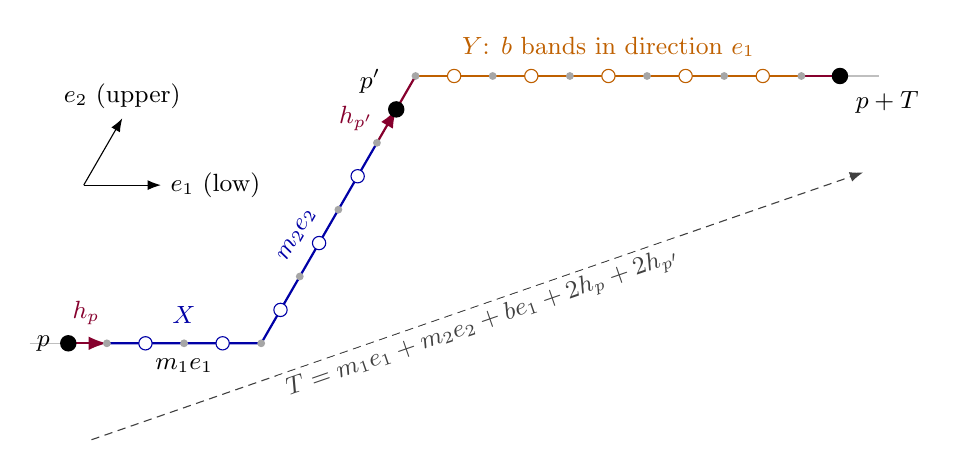
\begin{tikzpicture}[x=0.98cm,y=0.98cm,>=Latex,font=\small,
  ordinary/.style={circle,draw,fill=white,inner sep=1.7pt},
  marked/.style={circle,fill=black,inner sep=2.1pt},
  vertex/.style={circle,fill=black!35,inner sep=1pt}]
 \coordinate (p) at (0,0);
 \coordinate (a) at (0.5,0);
 \coordinate (bend) at (2.5,0);
 \coordinate (c) at (4,{1.5*sqrt(3)});
 \coordinate (pp) at (4.25,{1.75*sqrt(3)});
 \coordinate (d) at (4.5,{2*sqrt(3)});
 \coordinate (e) at (9.5,{2*sqrt(3)});
 \coordinate (pt) at (10,{2*sqrt(3)});

 \draw[thick,blue!65!black] (a)--(bend)--(c);
 \foreach \j in {0,1} {
   \node[ordinary,draw=blue!65!black] at ({1+\j},0) {};
 }
 \foreach \j in {0,1,2} {
   \node[ordinary,draw=blue!65!black]
     at ({2.75+0.5*\j},{(0.25+0.5*\j)*sqrt(3)}) {};
 }
 \node[blue!65!black,above] at (1.5,0.13) {$X$};
 \node[below] at (1.5,-0.08) {$m_1e_1$};
 \node[blue!65!black,rotate=60,above] at (3.15,1.3) {$m_2e_2$};

 \draw[black!25] (-0.5,0)--(p);
 \draw[thick,purple!70!black,->] (p)--(a);
 \draw[thick,purple!70!black,->] (c)--(pp);
 \draw[thick,purple!70!black] (pp)--(d);
 \draw[thick,purple!70!black] (e)--(pt);
 \draw[black!25] (pt)--(10.5,{2*sqrt(3)});
 \node[purple!70!black,above] at (0.23,0.12) {$h_p$};
 \node[purple!70!black,left] at (4.08,{1.68*sqrt(3)}) {$h_{p'}$};

 \draw[thick,orange!75!black] (d)--(e);
 \foreach \j in {0,1,2,3,4} {
   \node[ordinary,draw=orange!75!black]
     at ({5+\j},{2*sqrt(3)}) {};
 }
 \node[orange!75!black,above] at (7,{2*sqrt(3)+0.12})
   {$Y$: $b$ bands in direction $e_1$};

 \foreach \pos in {a,bend,c,d,e} \node[vertex] at (\pos) {};
 \node[vertex] at (1.5,0) {};
 \foreach \j in {1,2} {
   \node[vertex] at ({2.5+0.5*\j},{0.5*sqrt(3)*\j}) {};
 }
 \foreach \j in {1,2,3,4} {
   \node[vertex] at ({4.5+\j},{2*sqrt(3)}) {};
 }
 \node[marked,label={left:$p$}] at (p) {};
 \node[marked,label={above left:$p'$}] at (pp) {};
 \node[marked,label={below right:$p+T$}] at (pt) {};

 \draw[densely dashed,->,black!75]
   (0.3,-1.25)--(10.3,{2*sqrt(3)-1.25})
   node[midway,sloped,below,fill=white,inner sep=2pt]
     {$T=m_1e_1+m_2e_2+be_1+2h_p+2h_{p'}$};

 \begin{scope}[shift={(0.2,2.05)}]
   \draw[->] (0,0)--(1,0) node[right] {$e_1$ (low)};
   \draw[->] (0,0)--(0.5,{sqrt(3)/2})
     node[above] {$e_2$ (upper)};
 \end{scope}
\end{tikzpicture}
\caption{Constructing the cyclic cut from an ordered pair of visited
ports. Open circles are ordinary ports at the midpoints of complete
triangular sides; black circles are the marks. The $X$ part joins
$p+h_p$ to $p'-h_{p'}$ using $m_1$ sides in direction $e_1$ and
$m_2$ in direction $e_2$, in a fixed order. The complementary part has
$b$ ordinary sides in the low direction. The displayed mark types have
$h_p=e_1/2$ and $h_{p'}=e_2/2$; either half-side can have either
allowed direction. Identifying $p+T$ with $p$ closes the row on the
cylinder. Taking $|T|>2D$ makes projection injective on each planar
polygon of diameter at most $D$. Counts and lengths are illustrative.}
\label{fig:marked-row}
\end{figure}


The retained pairs have $s\gg D^{1/2}$, and the minority count is
$s(1-t)=\min(m_1,m_2)\gg D^{1/8}$. Consequently
\[
 L_X\ge\frac{\log D}{2\gamma}-O(1),\qquad
 L_Y=\frac{\log D}{\gamma}+O(1).
\]
Every fixed $0<c_1<1/2$ and $0<c_4<\gamma/8$ therefore gives
$L_X\ge c_1L_Y$ and $s(1-t)\ge e^{c_4L_Y}$ for all sufficiently
large $D$. These configurations meet the stated margins.

\par\smallskip\noindent\textbf{Counting the marked occurrences.}
Moving a vertex to an incident port has at most two inverse choices
at each endpoint. The choices of basis, rotation, reflection, and
port type also have bounded multiplicity. Normalize the first port
modulo triangular-lattice translations. Once its lift is fixed, the
projected polygon has a unique planar lift through that port, with
its original vertex weight. Thus the retained pairs account for at
least a fixed multiple of $|P|^2$ marked occurrences, and any one
marked cylinder polygon arises from at most a fixed number of these
occurrences.

For a dyadic displacement scale $S$, let $\mathscr R_{D,S}$ be the
row setups just constructed with $S\le s<2S$, and write
$\mathcal C_{\mathfrak r}$ for the corresponding marked correlation.
There are $O(S^2)$ setups: after fixing the first port type, there
are only $O(S^2)$ possible second-port displacements, and the
remaining choices are bounded. Positivity and the preceding
multiplicity bounds give
\[
 \sum_{\substack{[P]:\ D/2<\operatorname{diam}P\le D\\
                         |P|>D^{4/3}}}
       \rho_{\rm v}^{|P|}|P|^2
 \le C\sum_{\substack{S\ \text{dyadic}\\D^{1/2}\ll S\ll D}}
          \ \sum_{\mathfrak r\in\mathscr R_{D,S}}
                    \mathcal C_{\mathfrak r}.
\]
A bound of the stated form makes each displacement scale contribute
at most $D^{2/3+o(1)}$. The $O(\log D)$ scales and the
short-polygon estimate prove the claimed reduction.
\end{proof}

\section{Magnetic fluctuations and the rare central scale}
\label{sec:07_magnetic_analysis-fluctuations}

The trial bounds have reduced the problem to a reference integral with
fixed integer dimensions. Its Hessian sees the entire wall intervals
on the main contours, including the rare central scale. This differs from the preceding
smoothing estimates, where a same-main explicit particle can reach that
scale only through an exponentially small smoothing tail. We first
control the Hessian and its determinant at the rare scale. We then
choose a coordinate in which the trial fields can be implemented by
small particle motions, adapting the reference and contour arguments
of \cite{Electric} to the unequal magnetic walls.

\subsection{Reference coordinates and the relative Hessian}

We now implement \eqref{eq:M-23},\eqref{eq:M-24},\eqref{eq:M-29} under the parameter margins just stated. Retain the sizes $s_g$ and unit-mass mean densities $\bar\nu_g$ introduced in the trial setup. In this part no interpolation of dimensions, nor continuation in \(M\), is needed: use \(N_g=m'_g\) particles in the reference integral of group \(g\) (only nonnegative integer dimensions occur). All inner trial changes have zero mass separately by group. After the
polynomial count truncation justified in the proof of
Proposition~\ref{prop:07_magnetic_analysis-transport},
\(N_g=s_g+O(L^K)\) for a fixed \(K\), whereas
\(s_g=e^{\gamma L_g}\); hence \(N_g\asymp s_g\).
Phase factors depending only on counts have modulus one.

We may work on subsequences on which \(L_X/L\) and the mixture fraction \(t\) have limits. Call the case \(\lim t<1\), or \(t=1\) identically, regular. In the remaining case, passing to another subsequence, \(t<1,\ t\to1\); call this the rare case and use the scale \(d_0=\beta(1-\theta(0))\) from the curve estimates. Thus \(\log(1/d_0)=O(L)\), and \(s d_0\) grows at least as \(e^{cL}\) for some \(c>0\).

We first specify the cap maps used in the reference coordinates.
For an interval $[-\Lambda,\Lambda]$ choose a fixed $a_0=O(1)$
and an odd map $W:[-\Lambda-a_0,\Lambda+a_0]\to[-\Lambda,\Lambda]$.
At the positive endpoint write
$W(\Lambda+a_0-r)=\Lambda-\omega(r)$, where $\omega$ is quadratic
near zero, increasing with $\omega'(r)\asymp\min(r,1)$, and
$\omega(r)=r-a_0$ for $r\ge1$. Integrating a smooth cutoff between
$r$ and one constructs $\omega$ and fixes $a_0$. Thus $W(v)=v$
away from bounded endpoint neighborhoods and reflects evenly at the
endpoints.

Use first an \emph{unstretched} parameter $v$ per wall interval. In the regular case set the intermediate coordinate \(\xi=u\) on each, and use the cap map \(\xi=W_g(v)\) onto \([-L_g,L_g]\) using the cap construction just given for each separate length. Take the reference probability with density in \(v\)
\[
 \lambda_g^0(v)=C_g\,\eta_g(W_g(v)),\qquad \eta_g=\bar\nu_g .
\]
In the rare case do this on \(Y\) as usual, but on \(X\) set \(\xi=b_X(u)\) by the mean-matching map, use \(W_X\) onto \([-b_X(L_X),b_X(L_X)]\), and take \(\eta_X=\rho\). Write \(A_g\) for the unstretched positive endpoints and \(U_g(v)\) for the resulting map to \(u\). In all cases \(A_g=L_g+O(1)\), \(C_g=1+O(e^{-\gamma L_g})\). The push of the unnormalized density \(\eta_g(W_g(v))\,dv\) to \(u\) agrees with \(\bar\nu_g\,du\) away from or before the bounded-width cap regions (i.e. throughout the interior bulk); the cap and omitted tail masses are \(O(e^{-\gamma L_g})\) with exponential decay outside. Denote the normalized push by \(p_g\), and the reference angular coordinate by \(t_g(v)=\pi\int_{-A_g}^v\lambda_g^0\). The curve estimates show that the unstretched densities have uniform fixed-order relative derivative bounds, sizes comparable to $e^{-\gamma|v|}$, and uniform local analytic bounds off the caps. They extend evenly at the endpoints.

The coordinate maps are thus
\[
 v\ \xmapsto{\ W_g\ }\ \xi\ \longmapsto\ u=U_g(v),
 \qquad
 \xi=u\ \text{except on rare }X,\quad \xi=b_X(u)\ \text{there}.
\]
The contour point is $\mathfrak z_g(u)$, while $t_g(v)$ is the
reference angle. Densities are pushed through these maps. A primitive
instead composes with $U_g$: if $q_u=\partial_uQ_u$,
then $Q_v(v)=Q_u(U_g(v))$ and $q_u(u)\,du=\partial_vQ_v(v)\,dv$.
We use the same letter for these representations of a primitive.
Consequently $h_0$, the true quadratic form, and their relative
determinant do not change under a further reparametrization. The
unstretched coordinate $v$ will be used for the spectral calculation.

Use the reference space $\mathcal X$ of Section~\ref{sec:reference-law}
with these two angular variables. Compose the true $H_{nn}$ with the
maps $U_g$, subtract its diagonal reference kernel, and call the
mixed derivative of that smooth difference $\mathscr K$.
Thus $H_{\rm form}(Q,Q)=h_0(Q,Q)+(Q,\mathscr KQ)$ and
$T=I+j^*\mathscr K j$, where $j$ is inclusion in physical $L^2$.
We will prove the following spectral bounds:
\begin{equation}\label{eq:G-8}
 \begin{gathered}
 \|T-I\|_1\le CL,\quad\|T\|\le C,\quad
 A_T=(T+T^*)/2\ge cL^{-2}I,\\
 N_{A_T}(a)\le CL\sqrt a\quad(0<a<a_0).
 \end{gathered}
\end{equation}
The same gap and small-value count are required for singular values
and orthogonal compressions.

\subsection{Spectral bounds and the unequal-wall determinant}

The bounds above control the logarithm at small singular values; the
bulk symbols then determine its leading integral. We begin with the
local norm and cell estimates needed for that control.

The magnetic statements in Equation~\eqref{eq:G-8} will now be verified. The embedding \(j\) in unstretched \(L^2(dv)\) has uniformly bounded norm; \(jj^*\) is the labelwise kernel
\[
 G(v,v')=\frac1{2\pi^2}\log\frac{\sin((t_g(v)+t_g(v'))/2)}
                              {\sin(|t_g(v)-t_g(v')|/2)}.
\] The kernel $G$ has uniformly integrable logarithmic singularities and
exponential off-diagonal decay. Thus Schur's test gives a uniform bound
for $j$. We next prove the lower spectral bounds directly in these
magnetic coordinates, before computing the determinant.

For a primitive $Q=(Q_X,Q_Y)$ put $d_g(v)=A_g-|v|$ and define
\[
 \mathfrak e(Q)=\sum_g\left[
 \iint_{|v-v'|\le2}
 \frac{|Q_g(v)-Q_g(v')|^2}{|v-v'|^2}\,dv\,dv'
 +\int_{d_g(v)\le2}\frac{|Q_g(v)|^2}{d_g(v)}\,dv\right].
\]
The odd angular extension gives
\begin{equation}\label{eq:magnetic-local-norm}
 h_0(Q,Q)\le C(\mathfrak e(Q)+\|jQ\|_2^2),\qquad
 \operatorname{Re}H_{\rm form}(Q,Q)\ge c\mathfrak e(Q).
\end{equation}
For the first inequality, the angular difference kernels in physical
variables are
\[
 \frac{t'_g(v)t'_g(v')}{\sin^2((t_g(v)-t_g(v'))/2)},\qquad
 \frac{t'_g(v)t'_g(v')}{\sin^2((t_g(v)+t_g(v'))/2)}.
\]
The first is at most $C|v-v'|^{-2}$ locally and is exponentially
integrable away from the diagonal. The reflected kernel has the same
bound away from common endpoints; near an endpoint it is bounded by
the inverse square of the sum of endpoint distances. Integrating one
variable gives $C/d_g(v)$. These statements use the exponential
reference density and its relative derivative bounds, which are uniform
also after rare-center mean matching. They prove the first inequality.

For the second, push $Q_g$ to the physical $u$ coordinate and extend
by zero outside its wall. The real-energy theorem controls the Fourier
seminorm with multiplier $k^2/(1+|k|)$. This is equivalent to the local
difference seminorm with kernel $|u-u'|^{-2}$ and a fixed sufficiently
large distance cutoff, including the zero extension. Near a cap,
$U'_g(v)\asymp\min(1,d_g(v))$, and interactions with the exterior
zeros give
$U'_g(v)/(L_g-|U_g(v)|)\asymp1/d_g(v)$. When two endpoint distances
are comparable, change of variables preserves the local difference
kernel up to bounded factors. When they are not comparable, the
inequality $|Q(v)-Q(v')|^2\le2|Q(v)|^2+2|Q(v')|^2$ bounds the
missing part by the endpoint term. The mean-matching derivative is
uniformly comparable to one, so this argument also covers rare $X$.
This proves Equation~\eqref{eq:magnetic-local-norm}.

Partition each physical parameter interval into cells of lengths between
$1/2$ and one, and let $q_a$ be the mean on cell $a$. The local
seminorm bounds the sum of the cell variances and
$\sum_a|q_{a+1}-q_a|^2$. On a block of length comparable to $b\ge1$
whose total mean vanishes, discrete Poincar\'e gives
$\|Q\|_2^2\le Cb^2\mathfrak e(Q)$. The same estimate on a whole
wall, without a zero-mean condition, follows by controlling its first
and last cell means with the endpoint term. Since both interval
lengths are at most $CL$, Equation~\eqref{eq:magnetic-local-norm}
gives the global gap $cL^{-2}$.

For a threshold $a$ above a fixed multiple of $L^{-2}$, choose blocks
of length $b=c_0a^{-1/2}$ with small fixed $c_0$. Their zero-mean
conditions have codimension at most $CL/b$; on their common kernel
the Rayleigh quotient of $A_T$ is at least $a$. Min--max gives
$N_{A_T}(a)\le CL\sqrt a$. Below the global gap the count is zero;
changing constants covers the intermediate range. Compression cannot
increase this count. Finally, if a subspace satisfies
$\|TQ\|<a\|Q\|$, then
$\langle Q,A_TQ\rangle\le\|Q\|\|TQ\|<a\|Q\|^2$ on that
subspace. This gives the same count for singular values, including
compressions. We have therefore established the magnetic lower bounds
required in Equation~\eqref{eq:G-8}. The following determinant proof
supplies its norm and trace bounds, including the rare center.

\begin{lemma}[The magnetic fluctuation determinant]\label{lem:07_magnetic_analysis-determinant}
The relative Hessian satisfies \(\|T-I\|_1=O(L),\ \|T\|=O(1)\), and
\begin{equation}
 -\tfrac12\log|\det T|
 =\tfrac{7\gamma}{8}L_X+\tfrac{5\gamma}{16}(L_Y-L_X)+o(L).
 \label{eq:M-31}
\end{equation}
In the rare case, let \(T^0\) be the straight comparison with
main coordinates \(W_X(v)+i\beta,W_Y(v)\), using exactly the same
reference form \(h_0\). Then
\begin{equation}
 \|T-T^0\|=o(1),\qquad \|T-T^0\|_1=o(L).
 \label{eq:M-32}
\end{equation}
In particular all errors in \eqref{eq:M-31} are uniform along every subsequence
specified above, including \(t\uparrow1\).
\end{lemma}
\begin{proof}
\par\smallskip\noindent\textbf{Trace bounds for the straight comparison.}
In the rare case let \(T^0\) denote the straight comparison using physical main coordinates \(W_X(v)+i\beta,\ W_Y(v)\), and \emph{exactly the same} \(h_0\). In the regular case let \(T^0=T\). For \(T^0\) the mixed derivative of the true-minus-reference kernel has uniform \(C^j\) bounds of order \(C_j e^{-c|v-v'|}\), all fixed \(j\). Indeed on a regular curved main the same diagonal argument subtracts the horizontal log, the residual using the divided ratio for the curved \(\sinh\); it is uniformly regular including at caps by composition (the ratio of the two physical complex and horizontal differences before composing with \(W_X\) already extends smoothly with controlled log). Other near-diagonal entries are offset from their zero angles. At long differences the linear and sign asymptotes, including the terms from curved heights, are additive in individual coordinates in fixed order and vanish on mixed differentiation; the remaining log tails and the reference sine ratios obey the
same exponential estimates. To obtain the trace bound, partition each
interval into cells of lengths in $[1,2]$ and use their normalized
cosine bases $e_{a,n}$. Integrating twice by parts in each variable,
with the first boundary term zero and the second controlled by a
kernel derivative, gives
\[
 |\langle e_{a,n},\mathscr K e_{b,m}\rangle|
 \le \frac{Ce^{-c|a-b|}}{(1+n^2)(1+m^2)}.
\]
Summing the trace norms of these rank-one entries gives $O(L)$;
Schur's test gives an operator norm $O(1)$. Boundedness of $j$
transfers both statements to $T^0$.

\par\smallskip\noindent\textbf{The common and shoulder symbols.}
Cyclic kernel integrals then
give the word limits used below. More precisely, deep points \(|v|<L_X\), away from the center and edges by distances tending to infinity, see the common symbol \(T_\infty(k)\) there with \(p=(3-\lim\theta_\infty)\beta\) (angle 1 for the horizontal comparison in the rare case); see the main transform formulas. Indeed the reference densities in each tail are asymptotic with derivatives to a constant times \(e^{-\gamma |v|}\), and the curved height is exponentially asymptotic to \(\theta_\infty\). Deep points in \(L_X<|v|<L_Y\) see only its \(Y,Y\) entry. Their respective weights after division by \(2L\) are \(\lim L_X/L\) and the complement. Bounded-distance exceptional regions have zero limiting share, and relative-coordinate tails can be truncated uniformly by the kernel bounds. For completeness, its $2\times2$ expression, for $k>0$ and
$x=\beta k$, is
\[
 T_\infty(k)=\frac{2\cosh x-1}{\sinh(4x)\coth(3x/2)}
 \begin{pmatrix}\cosh(3x)&e^{pk}\\ e^{-pk}&\cosh(3x)\end{pmatrix};
 \qquad T_\infty(-k)=T_\infty(k)^{\mathsf t}.
\]
It is obtained by dividing the true primitive symbol $k^2\widehat H$
by the limiting reference symbol $2\pi k\coth(\pi k/(2\gamma))$.
Its determinant is independent of $p$, and, with $y=e^{-x}$,
\[
 \sqrt{\det T_\infty(k)}
 =\frac{(1-y^3)(1-y^6)}{(1+y)(1-y^8)}.
\]
The logarithmic integral is
\[
 \int_0^\infty\log\sqrt{\det T_\infty(x/\beta)}\,dx
 =-\frac{\pi^2}{18}-\frac{\pi^2}{36}
       -\frac{\pi^2}{12}+\frac{\pi^2}{48}
 =-\frac{7\pi^2}{48}.
\]
Each term follows by integrating the convergent logarithmic series.
Accounting for both signs of $k$, the determinant square, and the
common interval length $2L_X$ yields the contribution
$7\gamma L_X/8$ to $-\frac12\log|\det T|$.
The scalar shoulder symbol for \(x=\beta|k|,\ y=e^{-x}\) is
\[
 \frac{c_*(k)\cosh(3x)}{\sinh(4x)\coth(3x/2)}
 =\frac{(1-y^3)(1+y^6)}{(1+y)(1-y^8)}
\]
The integral of the logarithm of the shoulder symbol over
\(x\in(0,\infty)\) is
\[
 -\frac{\pi^2}{18}+\frac{\pi^2}{72}
 -\frac{\pi^2}{12}+\frac{\pi^2}{48}
 =-\frac{5\pi^2}{48},
\]
by expanding each logarithm in its absolutely integrable series. This gives \eqref{eq:M-31} by the same truncated-log argument once trace convergence holds also for \(T\), since \eqref{eq:G-8} was proved for \(T\).

\par\smallskip\noindent\textbf{Passing to the logarithmic determinant.}
Here is the truncated-log passage used in this calculation. For the
singular values $s_i(T)$, the small-value count gives
\[
 \sum_{s_i<\eta}\log(\eta/s_i)
 =\int_0^\eta\frac{\#\{s_i<r\}}r\,dr\le CL\sqrt\eta.
\]
Clipping $\log(T^*T)$ below $\eta^2$ therefore loses only
$O(L\sqrt\eta)$. On the bounded spectral interval, approximate the
clipped logarithm by polynomials vanishing at one, with error at most
$\epsilon|x-1|$. The trace error is at most
$\epsilon\|T^*T-I\|_1=O(\epsilon L)$. Cyclic kernel integration
proves the polynomial trace limits: truncate relative separations,
use the integrable logarithmic bound for $G$ and the exponential bounds
for $\mathscr K$, and then discard bounded neighborhoods of the center
and walls. The common interval occupies length $2L_X$ and the
shoulders length $2(L_Y-L_X)$. The same clipping estimate holds for
the displayed symbols. The common symbol has one singular value
comparable to $k^2$ near zero and its other singular value stays
positive; the scalar shoulder symbol tends to $3/8$ there. Both
symbols approach identity exponentially at infinity.
Take size to infinity, then $\epsilon\downarrow0$ and
$\eta\downarrow0$. The two logarithmic integrals give exactly the
coefficients in Equation~\eqref{eq:M-31}.

\par\smallskip\noindent\textbf{The rare-center comparison.}
It remains to prove the comparison uniformly at the rare central scale. Ordinary derivative bounds in \(v\) degenerate at that scale, so we use a dyadic decomposition. In intermediate coordinates put
\[
 \mathfrak z_X(b_X^{-1}(\xi))=\xi+i\beta+E(\xi).
\]
Then \(E,E'\) are \(o(1)\) uniformly, with fixed higher derivatives \(E^{(j)}=o(1)\,[\min(1,|\xi|+d_0)]^{1-j}\), by the graph and matching estimates. The kernel on primitives uses a mixed derivative of the difference \(K_d=H_{nn}-H_{nn}^0\) with the two sets of maps just described. Split \(X\), on \(|v|\le1\) (so \(W_X(v)=v\)), into sign-paired shells of radii \(r_j=2^{-j}\) down to \(r_J\asymp d_0\): \(r_{j+1}<|v|<r_j,\ j<J\), and the last central interval \(|v|<r_J\). In shell \(j\) encode \(Q_X\) by its oscillation from the single mean \(m_j\) over that shell, measured in \(L^2\) after rescaling the shell by \(r_j\), and keep the numbers \(m_0,\ m_j-m_{j-1}\). The means thus contribute to \(Q_X\) by these coefficients times the steps \(\mathbf1_{|v|<r_j}\). Outside this region and on \(Y\) keep \(Q\) itself in \(L^2\) on cells of lengths between 1 and 2. This joint encoding has squared norm bounded by \(C h_0(Q,Q)\). Indeed same- and adjacent-shell squared mean/oscillation differences are bounded in sum by the ordinary difference seminorm on \([-1,1]\), directly controlled there by the angular difference representation of \(h_0\); the outer mean and ordinary cells cost \(\|jQ\|^2\).
For example, with \(A_j=\{r_{j+1}<|v|<r_j\}\),
\[
 \frac1{r_j}\int_{A_j}|Q-m_j|^2
 \le C\iint_{A_j\times A_j}
        \frac{|Q(u)-Q(v)|^2}{|u-v|^2}\,du\,dv,
\]
and the same calculation on \(A_j\times A_{j+1}\) bounds
\(|m_j-m_{j+1}|^2\). These pair regions have bounded overlap.
The last central interval satisfies the same scaled estimate. Thus the
encoding map is bounded independently of the number of shells.

For oscillation or ordinary cells the matrix kernel on this encoding takes one derivative of \(K_d\) on the natural unit scale of each applicable variable (rescaled for shells). For a step, integrate that derivative over the step: take instead the difference of values at \(+r_j,-r_j\). Thus there is no cost from a large \emph{common} primitive mean at tiny scales. Each cell pair, including derivatives through two further orders per continuous variable, has bounds \(C\epsilon_L\) times:
\begin{itemize}
\item \(\min(r_i/r_j,r_j/r_i)\) between shells (steps are included at their corresponding scale);
\item \(r_j e^{-c|v'|}\) from shell \(j\) to an ordinary cell at \(v'\);
\item \(e^{-c|v-v'|}\) between ordinary cells;
\end{itemize}
where \(\epsilon_L=o(1)\).

To verify them, on two central \(X\) arguments the diagonal log change is a multiple of the smooth log of \(1+(E(v)-E(v'))/(v-v')\) plus regular analytic changes. For comparable scales this has all required bounds by divided differences at nearby arguments in the same regular neighborhood of radius of that scale (including the innermost pair), or by separation otherwise. For a much smaller scale \(r_i\ll r_j\) differentiation on the smaller scale gains \(r_i/r_j\), since the denominator has size \(r_j\) and all positive-order normalized derivatives of \(E\) on the smaller shell have size \(C\epsilon_L r_i\); further derivatives on either scale preserve the bound. A step difference gains the same by varying its argument across \([-r_i,r_i]\), using only the uniform slope bound for \(E\) there. The larger step endpoints themselves stay on the larger scale. The argument across the interface to ordinary \(X\) cells is identical; a bounded-distance ordinary \(Y\) argument instead sees a nonsingular analytic kernel. In far-separated comparisons the pure one-variable log asymptotes drop out after the two derivatives/differences, including when one uses step endpoints (order with the other far argument is fixed); the log series remainders give exponential decay along with the small change bounds, with the scale gain from a central derivative or step. On ordinary \(X\) cells near a cap the divided differences for the change use \(E(\xi)-E(\xi')\) divided by \(\xi-\xi'\) \emph{before} the cap map, so do not incur any endpoint derivative loss. These observations prove the stated estimates for the log branches continued by the graph deformation; additive constants do not enter.

By smooth cell expansion (e.g. the same cosine trace bound as before, on the two separate sign components where needed), these are also trace-norm bounds per pair. Their row and column sums are \(O(\epsilon_L)\), and their overall sum \(O(\epsilon_L(L+J))\). Factoring on both sides by the bounded encoding proves \eqref{eq:M-32}. Consequently the needed trace bounds and word limits transfer to \(T\) (trace-norm comparison of products), proving \eqref{eq:M-31}.


Since \(J=O(1+\log(1/d_0))=O(L)\), the shell-pair trace estimate is
indeed \(o(L)\). To transfer a word of fixed length in \(T-I,T^*-I\),
expand its difference from the corresponding word in \(T^0\) as a
sum with one difference factor in each summand. The trace norm is
\(o(L)\), because all other factors have bounded operator norms.
The small-singular-value count in Equation~\eqref{eq:G-8} controls the
removed portion of the logarithm uniformly, so no uniform pointwise
inverse bound at the rare scale is required.

\end{proof}

\subsection{A finite core and regular coordinates}

The determinant estimate controls the global cost. To realize the trial
field by moving actual particles, we next choose a finite core and a
coordinate in which its fields, dual tests, and density have uniform
regularity.

Fix a small tolerance $\xi>0$. We construct a real orthogonal
projection $\Pi$ of rank $O_\xi(L)$, supported on each label in
$|v|<(1-\delta_*)L_g$ for a fixed $\delta_*>0$, such that
\begin{equation}\label{eq:G-10}
 \|T-I-\Pi(T-I)\Pi\|_1\le\xi L.
\end{equation}
Apply the smooth-core construction of \cite[Lemma~3.11]{Electric}
to $T^0$. Its cell approximation uses the compensated-kernel bounds
proved above. It then applies the reference inverse $G$ to smooth
cell functions and cuts off the resulting fields inside the walls.
The exponential decay of $G$ makes this cutoff error negligible;
discarding the outer $O(\delta_*L)$ cells costs $O(\delta_*L)$ in
trace norm. These arguments apply separately on our two intervals.
On rare $X$, both $G$ and the reference density in $v$ remain regular,
so the constructed orthonormal fields have polynomial fixed-order
derivative bounds in $v$. To pass from $T^0$ to $T$, use
\[
 \|(T-I)-\Pi(T-I)\Pi\|_1
 \le \|(T^0-I)-\Pi(T^0-I)\Pi\|_1+2\|T-T^0\|_1.
\]
Choosing the initial tolerance smaller and using
Equation~\eqref{eq:M-32} proves Equation~\eqref{eq:G-10}.

Write $S=\operatorname{ran}\Pi$, $R=S^\perp$ and
$T_e=T_{RR}-T_{RS}T_{SS}^{-1}T_{SR}$. Its Hermitian part
$\operatorname{Re}T_e$ inherits the gap and small-value count in
Equation~\eqref{eq:G-8}. The accompanying comparison is
\begin{equation}\label{eq:G-11}
 \begin{aligned}
 |\log|\det T_{SS}|-\log|\det T||&=o_\xi(L),\\
 \sum_{\lambda<1,\ \lambda\in\operatorname{spec}\operatorname{Re}T_e}
             -\log\lambda&=o_\xi(L).
 \end{aligned}
\end{equation}
Here the normalized limsup tends to zero when $\xi\downarrow0$
after $L\to\infty$. These conclusions follow from
\cite[Lemma~3.12]{Electric}, whose operator argument uses precisely
Equation~\eqref{eq:G-10} and the magnetic gap and small-value counts
already proved. In particular it controls the negative logarithms of
$\operatorname{Re}T_e$, not only the determinant of $T_e$.

The core fields themselves are now regular in $v$. Their images under
the true form can still vary on the rare scale. The next change of
coordinate controls these dual tests as well as the particle motion;
it preserves the forms and the projection just constructed.


\begin{lemma}[A regular parameter for transport]\label{lem:07_magnetic_analysis-stretch}
On rare $X$, define $\tau(0)=0$ and
\[
 \frac{d\tau}{dv}=1+\frac1{\sqrt{d_0^2+W_X(v)^2}};
\]
on the other intervals set $\tau=v$. Let $\widetilde A_g$ be the
new endpoints and $\lambda_g(\tau)=\lambda_g^0(v)\,dv/d\tau$ the
reference probability density. Then $\widetilde A_g\asymp L$,
$|\log\lambda_g|=O(L)$, and $\lambda_g$ has smooth even endpoint
reflections with uniformly bounded relative derivatives of every
fixed order. Off the bounded-width caps, the maps extend analytically
to fixed small disks in $\tau$. In those disks the density has relative
bounds, and increments and positive-order derivatives of $v$, $U_g$,
and $\mathfrak z_g(U_g)$ are bounded on the scale $dv/d\tau$.
For every fixed $\delta_*>0$, if $N_g\asymp s_g$, then
\begin{equation}\label{eq:M-33}
 N_g\lambda_g(\tau)\ge e^{c(\delta_*)L}
 \qquad\text{on }|v|\le(1-\delta_*)L_g
\end{equation}
for all sufficiently large sizes.

Suppose also that $n_e,\ell_e,|M|$ are bounded by fixed powers of $L$.
In the $\tau$ coordinate the following data have polynomial bounds
for every fixed derivative order:
\begin{itemize}
\item the compensated kernel $H_{nn}-H_{\rm ref}$, with smooth even
endpoint reflections and analytic continuations in its core variables;
\item the linear density test
$H_{nn}(m'p_L-\mu)+\widetilde H_{ne}\zeta-\mathfrak t_n$, with the
same reflections and core analyticity;
\item the smooth dual tests obtained by applying $h_0$ or
$H_{\rm form}$ to the core basis fields or the trial primitives.
These tests have odd reflections when paired against primitives.
\end{itemize}
The constant term of $\operatorname{Re}\mathcal D$ on $m'p_L$ is
bounded below by $-{\rm poly}(L)$. The core density bound also holds
where a trial primitive is nonzero through the center.
\end{lemma}
\begin{proof}
\par\smallskip\noindent\textbf{Local scale and density.}
On rare $X$,
\[
 \frac{dv}{d\tau}\asymp\min(1,d_0+|v|).
\]
The added length near the center is
$O(1+\log(1/d_0))=O(L)$. Thus the intervals still have length
comparable to $L$. In a $v$-disk of radius $c(|v|+d_0)$ near the
center, the derivative of $\tau$ has small relative variation when
$c$ is small. Analytic inversion, together with the graph and
mean-matching estimates on that same scale, gives the claimed fixed
$\tau$-disks. At the caps the stretch is smooth and respects the
reflections; analytic continuation there is not needed.

The identity $\lambda_g=\lambda_g^0\,dv/d\tau$ gives the logarithmic
and relative derivative bounds. On $|v|\le1$ in rare $X$ it gives
\[
 N_X\lambda_X\ge c s d_0\ge e^{c'L},
\]
using the minority margin. Away from this central region, throughout
a core,
\[
 N_g\lambda_g\ge c s_g e^{-\gamma(1-\delta_*)L_g}
       =c e^{\gamma\delta_*L_g}.
\]
These two estimates prove Equation~\eqref{eq:M-33}. In particular
one need not remove the center from the support of a primitive.

\par\smallskip\noindent\textbf{Compensated logarithms.}
Consider first two points on the same label. If their $\tau$-distance
is at least a fixed $c_0>0$, their horizontal physical separation is
at least a constant times either local scale $dv/d\tau$. This follows
by integrating the local scale on a fixed subinterval; it remains true
at a cap, where the physical derivative can vanish at the endpoint.
Likewise the sine of half the angular difference bounds both local
$\lambda_g$ from below up to constants. The sine of the angular
half-sum is at least as large. The logarithms and their derivatives
therefore have the asserted bounds away from the local diagonal.

Near the diagonal, divide both physical and reference differences by
$\tau-\tau'$. Off the caps, the physical complex quotient has size
comparable to $dv/d\tau$, while the reference cosine quotient has
size comparable to $\lambda_g\sin t_g$; here
$\sin t_g\asymp\lambda_g^0$ away from the endpoints. Their relative
analytic derivative bounds follow from divided differences on the
fixed disks just constructed. At an endpoint, divide also by the
reflected coordinate difference. The quadratic cap maps make both
quotients smooth, nonzero on their natural scales, and even under
reflection. Their logarithmic ratio is consequently smooth through
both diagonals. Cross-label factors and the remaining same-label
factors stay at regular imaginary offsets when their real arguments
approach. Shrinking the core disks preserves those separations.
This proves the bounds and core analyticity for
$H_{nn}-H_{\rm ref}$.

\par\smallskip\noindent\textbf{Linear sources and end corrections.}
For each label decompose the signed measure $m'_gp_g-\mu_g$ into
$(m'_gC_g-s_g)\bar\nu_g\,du$ plus $m'_gC_g$ times the difference
between the unnormalized capped push and $\bar\nu_g\,du$.
The first coefficient is polynomial. Its convolution is given by
the mean identities, so it consists of ordinary $V$-logs evaluated
on the contour. The only possible shrinking site-pole distance is
at the rare $X$ center. There it is bounded below by a constant times
$|u|+d_0$, exactly the local scale controlled by $\tau$.

For the difference of measures, insert a fixed-width cutoff around
the caps and their exterior tails. The measures agree off this set,
and their densities in their respective parameters carry the factor
$e^{-\gamma L_g}$. In a same-label end convolution, subtract the
ordinary local logarithm and its reflected term for the capped input.
The curved divided-log remainder is regular. Derivatives of the
singular logarithm transfer to the smooth cutoff density, using its
even extension for the capped input; for the full-line input transfer
derivatives in $u$ before composition. Multiplication by $m'_g$ thus
leaves polynomial bounds. The end correction is analytic in core
variables by spatial separation on the same label and by imaginary
offsets on the other label.

The explicit-particle term $\widetilde H_{ne}\zeta$ uses the regular
offsets and horizontal subtraction from Equation~\eqref{eq:M-21}.
Its subtraction $R_h$ is inactive on moving core variables. The anomaly
logs have the uniform offsets established in the mean calculation.
These observations prove the linear-test assertion. Its constant
term has the stated lower bound by Equation~\eqref{eq:M-23}.

\par\smallskip\noindent\textbf{Dual tests and polynomial approximation.}
Against a smooth density supported in the core, subtract the local
$\tau$-diagonal logarithm of $H_{\rm ref}$ and transfer its derivatives
to the density. The remaining kernel has the bounds just proved.
Thus $H_{\rm ref}$ maps these densities to smooth even tests with
polynomial derivatives. The basis fields were constructed with
polynomial derivatives in $v$, hence also in $\tau$. The trial
primitives have the same property by Equations~\eqref{eq:M-24},
\eqref{eq:M-26} and~\eqref{eq:M-27}. Differentiating their density
tests gives the odd-reflected primitive tests for $h_0$. Adding the
smooth compensated kernel gives those for the true $H_{\rm form}$.
This last step is why no polynomial derivative bound for the true
form in the unstretched rare coordinate is needed.

We will also use physical sine approximation on the $\tau$ intervals.
Two estimates ensure that its errors remain polynomial. First,
$\mathcal X\hookrightarrow L^2(d\tau)$ has polynomial norm:
the inverse kernel satisfies
\[
 |G(\tau,\tau')|\le C\bigl(L+
       |\log\min(1,|\tau-\tau'|)|\bigr)
\]
by the exponential lower bound on $\lambda_g$, and Schur's test
applies on intervals of length $O(L)$. Second, $h_0$ is polynomially
bounded on unit vectors in every polynomial Dirichlet sine bandwidth.
For this use the angular difference kernel with its density factors.
Its unreflected part is at most
$C(1+|\tau-\tau'|^{-2})$, by the relative density derivative bounds.
The reflected part contributes an endpoint inverse-distance mass term,
since
\[
 \sin t_g\ge c\lambda_g\min(1,\widetilde A_g-|\tau|),
\]
and its density-weighted kernel is bounded outside pairs near the same
endpoint. Sine functions vanish
at the endpoints, so these local difference and boundary estimates
give the asserted bandwidth bound.
\end{proof}

\subsection{Source and compensated quadratic estimates}\label{sec:reference-integration}

The preceding construction gives the concrete magnetic coordinates and
trial form. We now state the two reference-law bounds used to integrate
that form, retaining the partition masses from
Equation~\eqref{eq:reference-normalization}.

\begin{proposition}[Reference sources]\label{prop:reference-source}
For fixed $C_1$, integer dimensions $0\le N_g\le C_1e^{\gamma L}$,
and a real smooth reflected test $\ell(Q)$,
\begin{equation}\label{eq:G-13}
 \log\mathbb E_0 e^{\ell(Q)}\le C_2L+\tfrac12\|\ell\|_*^2.
\end{equation}
If $\ell(Q)=(f,q)$ and
$f_g(t)=f_{g,0}+2\sum_{k\ge1}f_{g,k}\cos kt$, then
$\|\ell\|_*^2=\sum_{g,k\ge1}k|f_{g,k}|^2$.
Constants in $f$ do not affect the test.
\end{proposition}

This is the reference-source estimate of
\cite[Theorem~4.2]{Electric}: comparison to the reflected circle
integral gives the displayed Gaussian term, and the reciprocal factors
$J_{N_g}^{-1}$ give the $O(L)$ normalization cost. The circle inequality
is a finite strong Szeg\H{o} bound \cite{Simon2005Szego}; its
Schur-polynomial proof is related to the unitary trace-moment argument
of Diaconis and Evans \cite{DiaconisEvans2001}.

For the sharp bound we need to remove this $O(L)$ normalization cost.
Set
\[
 \mathcal G=\{\|Q\|_{-2,\widetilde A}\le L^D\},
\]
where the negative norm uses squared weights
$(1+(n/\widetilde A_g)^2)^{-2}$ in the orthonormal sine basis of
each $\tau$ interval. The event may couple the two labels.
For fixed $D$, dimensions $N_g\asymp s_g$, and smooth even-reflected
physical tests $f_g(\tau)$ whose fixed-order derivatives have specified
polynomial bounds, we claim
\begin{equation}\label{eq:G-14}
 \log\mathbb E_0[\mathbf1_{\mathcal G}e^{\ell(Q)}]
 \le o(L)+\tfrac12\|\ell\|_*^2.
\end{equation}
The error is uniform when these powers and dimension-comparison
constants are fixed. Theorem~4.3 of \cite{Electric} proves the
corresponding electric statement. We adapt its change of variables
here, since the unequal walls and the rare center affect both the
motion and the normalization gain.

Choose a smooth primitive $0\le a_g\le1/4$, equal to $1/4$ on
$|v|\le(1-2\delta)L_g$ and zero before
$|v|=(1-\delta)L_g$, with monotone slow switches in $v$. For the two signs
$\epsilon=\pm1$ make the real changes of variables
\[
 F_{g,\epsilon}(\tau)
       =\tau-\epsilon\frac{a_g(\tau)}{N_g\lambda_g(\tau)}.
\]
These are increasing diffeomorphisms, equal to the identity near the
endpoints. Their displacements and all required fixed derivatives are
exponentially small by Equation~\eqref{eq:M-33}, including across the
center. The cosine-difference ratios extend smoothly through the
same-label diagonal by analytic division. Off that diagonal the sine
separation estimates in Lemma~\ref{lem:07_magnetic_analysis-stretch}
give the same exponentially small derivative bounds. Thus their errors
paired with $Q$ or $Q\otimes Q$ are $o(1)$ on $\mathcal G$.
Convolutions of $H_{\rm ref}$ with the smooth mean-push remainders
have the same bounds by local-log subtraction. These are the error
estimates used in the proof of \cite[Theorem~4.3]{Electric}, now in
$\tau$.

Write $\mathfrak g_g=\log\cot(t_g/2)$ and
\[
 G_g=(\mathfrak g_g,a_g')-\tfrac12h_0(a_g,a_g),
\]
with the form restricted to label $g$. The one-coordinate density
ratio cancels the omitted half-diagonal in the Vandermonde log change.
As in that proof, pulling back the tilted density with angular weight
$2(1+\epsilon\cos t_g)$ instead of $2\sin t_g$ gives its original
density times
\[
 \exp\left\{\epsilon\bigl[(\mathfrak g_g,X_{N_g})
          +(f_g,a_g')-(q_g,H_{\rm ref}a_g')\bigr]+G_g+o(1)\right\}
\]
on $\mathcal G$. Only core derivatives of $\mathfrak g_g$ occur,
since the motion vanishes near the endpoints.

The gain is most simply calculated in the unstretched $v$ coordinate.
There $-\mathfrak g_g'=t_g'/\sin t_g\to\gamma$ in either tail,
so
\[
 (\mathfrak g_g,a_g')=\gamma\int a_g(v)\,dv+o_\delta(L).
\]
On the support of the switches, two points in the same tail satisfy
\[
 H_{\rm ref}(t_g(v),t_g(v'))
 =4\gamma\min(|v|,|v'|)
   +O\bigl(1+|\log\min(1,|v-v'|)|\bigr),
\]
whereas opposite-tail values are bounded. This follows by factoring
the difference of the squared exponentially small distances to the
nearest angular endpoint. The identity
\[
 \iint_{[0,\infty)^2}\min(r,r')b'(r)b'(r')\,dr\,dr'
       =\int_0^\infty b(r)^2\,dr
\]
and the slow switches therefore give
\[
 h_0(a_g,a_g)=4\gamma\int a_g(v)^2\,dv+O_\delta(1),
 \qquad
 G_g\ge\frac{\gamma L_g}{4}-O(\delta L)-o_\delta(L).
\]
In particular the extra length introduced by the central stretch
has no effect on this coordinate-invariant energy.

Use the \emph{same} sign $\epsilon$ for both labels before taking
the geometric mean. The terms odd in $\epsilon$ cancel on the single
event $\mathcal G$. Cauchy--Schwarz, removal of that event from the
two positive integrals, and the circle comparison then give
\[
 \log\mathbb E_0[\mathbf1_{\mathcal G}e^{\ell(Q)}]
 \le-\sum_gG_g-\sum_g\log J_{N_g}
       +\tfrac12\|\ell\|_*^2+o(1).
\]
Since $-\log J_{N_g}=\gamma L_g/4+O(1)$, the excess over the
Gaussian term is $O(\delta L)+o_\delta(L)$. Taking $L\to\infty$
and then $\delta\downarrow0$ proves Equation~\eqref{eq:G-14}.

\begin{proposition}[Compensated quadratic integration]
\label{prop:quadratic-integration}
Let $F$ be real symmetric and bounded on $\mathcal X$, with
$F\ge gI$, $g>0$, and $F-I$ trace class. Suppose its perturbation
and a real linear functional $h_0(l,\cdot)$ are represented by smooth
reflected physical kernels and tests. Let $c\in\mathbb R$. For
\[
 V(Q)=c+h_0(l,Q)+\tfrac12h_0(Q,(F-I)Q),\qquad
 m_F=c-\tfrac12h_0(l,F^{-1}l),
\]
one has
\begin{equation}\label{eq:G-18}
 \log\mathbb E_0e^{-V(Q)}\le -m_F+C_2L
        +\tfrac12\sum_{\lambda<1,\ \lambda\in\operatorname{spec}F}
                   -\log\lambda.
\end{equation}
The sum counts multiplicity. If the sharper source bound
\eqref{eq:G-14} holds, the gap is inverse-polynomial, and the data
and required fixed-order derivatives have polynomial bounds, the
same estimate on $\mathcal G$ has $o(L)$ in place of $C_2L$.
\end{proposition}

For clarity, the cancellation underlying this import is short.
Set $Q_*=-F^{-1}l$ and $J=(I-F)_+$. Completing the square gives
\[
 -V(Q)\le-m_F+h_0(Q_*,Q)-\tfrac12\|Q_*\|^2
              +\tfrac12h_0(Q-Q_*,J(Q-Q_*)).
\]
Linearize the last term with a real Gaussian vector $g_J$ of covariance
$J$, and apply Proposition~\ref{prop:reference-source} to
$Q_*+g_J$. The mixed terms cancel exactly, leaving
$e^{-m_F+C_2L}\mathbb E e^{\|g_J\|^2/2}
=e^{-m_F+C_2L}\det(I-J)^{-1/2}$. Smooth finite-dimensional
approximation, gap control and Fatou's lemma give the stated general
form, as in \cite[Lemma~4.4]{Electric}. For its sharpened version,
use physical sine truncation in $\tau$. The two Sobolev estimates at
the end of Lemma~\ref{lem:07_magnetic_analysis-stretch} give polynomial
operator and dual-test bounds on every polynomial bandwidth. Smoothness
then makes the truncation error smaller than any prescribed inverse
power of $L$, both on $\mathcal G$ and after division by the gap.
Equation~\eqref{eq:G-14} applies to the resulting polynomially bounded
Gaussian sources; outside a sufficiently large polynomial ball use
Equation~\eqref{eq:G-13} and the Gaussian tail. This is the approximation
argument of that lemma with our physical coordinate.

\subsection{The finite-rank transport construction}

The remaining step is to realize the complex trial field in the
particle integral. We adapt the three-stage deformation proved in
\cite[Lemma~5.2]{Electric}. Its statement concerns electric sectors;
below we give the affine path for the magnetic form, prove its gap
bounds, and check the geometric estimates needed for the same contour
argument. Particle dimensions stay fixed throughout.

For fixed explicit configuration $\zeta$, define the quadratic cost
$\mathscr C_0(Y)=\mathcal D(m'p_L+Y',\zeta)$, where density
 derivatives are pushed from the regular coordinate to the physical one.
For a real smooth trial primitive $Z_0$ supported in the active core,
write
\[
 C_z(Y)=\mathscr C_0(Y+iZ_0)
       =c_z+h_0(u_z,Y)+\tfrac12h_0(Y,TY),\qquad
 m_z=\inf_{Y\ {\rm real}}\operatorname{Re}C_z(Y).
\]
The endpoint of the affine transformation is
\begin{equation}\label{eq:G-19}
 Q+a(Q)=iZ_0+Q_R+T_{SS}^{-1/2}Q_S
       -T_{SS}^{-1}\Pi u_z-T_{SS}^{-1}T_{SR}Q_R.
\end{equation}
The square root is the principal branch in the right half-plane,
well-defined by accretivity. The corresponding motion of a coordinate
$r$ of label $g$ is $-a_g(Q)(r)/(N_g\lambda_g(r))$.
Throughout this motion each $N_g$ is a fixed nonnegative integer.

The following proposition bounds the resulting magnetic integral,
including its two unnormalized reference masses.

\begin{proposition}[Implementation of magnetic trial actions]\label{prop:07_magnetic_analysis-transport}
Let \(Z_0\) be the primitive of the coarse or sharp tilt, and set
\[
 C_z(Y)=\mathcal D(m'p_L+(Y+iZ_0)',\zeta),\qquad
 m_z=\inf_{Y\in\mathcal X\text{ real}}\operatorname{Re}C_z(Y).
\]
Derivatives here denote densities pushed from \(\tau\) to the physical
coordinate. After the reference transport, the logarithm of the modulus
of the unnormalized sector integral is at most
\[
 -m_z+\tfrac{7\gamma}{8}L_X+\tfrac{5\gamma}{16}(L_Y-L_X)
       -\tfrac{\gamma}{4}(L_X+L_Y)+o_{\rm proj}(L)+o(L).
\]
The discarded part can be made smaller than
\(\exp(-L^{E_2})\) for any required fixed \(E_2\). The coefficient of
\(o_{\rm proj}(L)\) is arbitrarily small after the core projection is
improved. Without a tilt one also has the bound \(-m_0+O(L)\),
which permits polynomial truncation of \(n_e,|M|,\ell_e\).
\end{proposition}
\begin{proof}
\par\smallskip\noindent\textbf{Coarse integration and count truncation.}
For any chosen tilt, the infimum $m_z$ satisfies its deterministic
trial lower bound: first test smooth real fields, then use continuity
in $\mathcal X$. For $Z_0=0$, take absolute values and apply
Proposition~\ref{prop:quadratic-integration} with
$F=\operatorname{Re}T$. The smooth compensated data are defined at
fixed sizes even before polynomial truncation. The spectral bounds
and $\|T-I\|_1=O(L)$ give an $O(L)$ negative-log sum, and the
reference masses $J_{N_g}$ are bounded above. Thus the logarithm of
the unshifted integral is at most $-m_0+O(L)$.

Combining this with Equations~\eqref{eq:M-20} and~\eqref{eq:M-23}
retains damping in
$\ell_e+(M^2+n_e^2)/L$, apart from $C_{h,\varepsilon}(L+n_e)$.
Sum the Gaussian damping in $M$ and the position damping with the
factorial measures as in Equation~\eqref{eq:M-30}. We may thereby
restrict $n_e,|M|,\ell_e$ to sufficiently large fixed powers of $L$
with error $\exp(-\omega(L))$ at the extracted-product normalization.
Fix these powers from now on. Then $N_g=s_g+O(L^K)\asymp s_g$,
and all kernels, dual tests, and lower bounds for constant terms have
the polynomial controls proved above. The sharp source estimate
\eqref{eq:G-14} is available in $\tau$.

\par\smallskip\noindent\textbf{The affine path and its real gap.}
Put
\[
 \mathsf A=T_{SS},\qquad \mathsf C=T_{SR},\qquad
 \mathsf B=\mathsf A^{-1}\mathsf C,
 \qquad H_\vartheta=(1-\vartheta)I+\vartheta\mathsf A,
 \quad D_\vartheta=H_\vartheta^{-1/2}.
\]
For $0\le\vartheta\le1$, the three successive output primitives are
\[
\begin{aligned}
 &Q+i\vartheta Z_0,\\
 &iZ_0+Q_R+Q_S
       -\vartheta(\mathsf A^{-1}\Pi u_z+\mathsf BQ_R),\\
 &iZ_0+Q_R+D_\vartheta Q_S
       -\mathsf A^{-1}\Pi u_z-\mathsf BQ_R.
\end{aligned}
\]
The stages join at their endpoints, and the last endpoint is
Equation~\eqref{eq:G-19}. Accretivity places the spectrum of
$H_\vartheta$ in the right half-plane. The resolvent representation
of its principal inverse square root gives polynomial bounds on
$D_\vartheta$ and its required parameter derivatives, using
Equation~\eqref{eq:G-8}. Flattening the parameter at the joins
produces a smooth path.

We verify the real Hessian along this path. Write
$T[Y,Y]=h_0(Y,TY)$ with the complex bilinear convention.
The first stage changes only the source. For real $s\in S,r\in R$,
the second-stage linear map satisfies the exact identity
\[
 T[(s-\vartheta\mathsf Br,r),(s-\vartheta\mathsf Br,r)]
 =T[(s,(1-\vartheta)r),(s,(1-\vartheta)r)]
       +(2\vartheta-\vartheta^2)T_e[r,r].
\]
Both real forms on the right have the magnetic gap, and the two
coefficients of $\|r\|^2$ add to one. At the third stage the
Hessian is block diagonal, with blocks $T_e$ and
$\mathsf A H_\vartheta^{-1}$, because $D_\vartheta$ commutes with
$\mathsf A$ and is symmetric. The Hermitian identity
\[
 H_\vartheta^*\operatorname{Re}(\mathsf A H_\vartheta^{-1})
       H_\vartheta
 =(1-\vartheta)\operatorname{Re}\mathsf A
       +\vartheta\mathsf A^*\mathsf A
\]
gives an inverse-polynomial gap throughout this stage as well.
All nontrivial input uses of $Q$ are through smooth dual tests; all
output changes lie in $S+\mathbb C Z_0$ and are core-supported.
Their polynomial bounds follow from the core construction and the
stretched regularity lemma. The path changes the Hessian by finite
rank $O(L)$, so its trace norms and lower bounds for minimizing costs
are polynomial too.

At the endpoint, the real Hessian is
$I_S\oplus\operatorname{Re}T_e$. Its real infimum is at least $m_z$.
Indeed, for fixed real $r$, the complex stationary point of
$C_z(s+r)$ in $S$ is
$s_*=-\mathsf A^{-1}(\Pi u_z+\mathsf Cr)=s_1+is_2$. Completing
that square gives
\[
 \operatorname{Re}C_z(s_*+r)
 =\operatorname{Re}C_z(s_1+r)
       +\tfrac12h_0(s_2,\operatorname{Re}\mathsf A\,s_2)
 \ge m_z.
\]
The remaining endpoint input adds $\|s\|^2/2$.

\par\smallskip\noindent\textbf{The particle chain and its pole distances.}
Write $a_\vartheta(Q)$ for the output change along the flattened
path. Choose a smooth cutoff $\chi$, equal to one on $[0,1]$ and
zero on $[4,\infty)$, and use the parameter
\[
 \vartheta(Q)=\chi(\|Q\|_{-2,\widetilde A}^2/L^{2D}).
\]
Thus configurations in $\mathcal G$ undergo the full path, while
those outside $\|Q\|_{-2,\widetilde A}\le2L^D$ remain fixed.
For $a(Q)=a_{\vartheta(Q)}(Q)$, move a particle at $\tau$ by
\[
 \Delta_g(\tau;Q)=-\frac{a_g(Q)(\tau)}{N_g\lambda_g(\tau)}.
\]
The homotopy uses $a_{\upsilon\vartheta(Q)}(Q)$ for
$0\le\upsilon\le1$.
The exponent $D$ will be chosen after the polynomial truncations.
For fixed $D$, Equation~\eqref{eq:M-33} makes $\Delta_g$ and its
fixed-order spatial derivatives exponentially small, with $Q$ and
the cutoff parameter frozen for these derivatives.

On rare $X$, a fixed small $\tau$-disk corresponds to physical
increments on scale $dv/d\tau\asymp\min(1,d_0+|u|)$ in the core.
Hence the physical particle displacement is exponentially small
relative to $d_0+|u|$ near the center. The nearest site pole has at
least that distance by the stretched regularity lemma. All other
poles have fixed separation there. The compensated kernels and maps
therefore remain analytic on the moving chains, including against
inactive coordinates. Same-label coincidences are Vandermonde zeros;
the divided difference of the compensated ratio extends analytically
through them.

The exact contour argument of \cite[Lemma~5.2]{Electric} now applies
to these chains. Its maps need only be $C^2$ in the real particle
variables. This holds here because a particle's first and second
variations of its empirical primitive are $-\delta_\tau$ and
$\delta_\tau'$, both continuous in the physical $H^{-2}$ space.
Holomorphy is required of the density times volume form, not of the
smooth core fields defining the chain.

To see that the one nonholomorphic factor causes no difficulty,
partition every coordinate into a slightly enlarged active core and
its complement, and freeze the complementary coordinates. A like-main
explicit particle lies outside its own wall, whereas $R_h$ is
supported at horizontal distance at most one. Thus
$A=\exp(-(X_{\rm int},R_h\zeta))$ is independent of every active
coordinate. Factor it out before applying Stokes' theorem to the
remaining holomorphic top form. The displacements vanish near the
core boundaries, so the side faces of the homotopy contribute zero.
Only after this contour equality do we use $0\le A\le1$.

\par\smallskip\noindent\textbf{Compensated cost and finite Jacobian.}
We indicate why the error estimates in that contour proof persist
in $\tau$. Freeze $Q$ and $a$, and multiply $\Delta$ by a scalar
complex parameter. Its analytic disk can have exponentially large
radius: the motion stays inside the fixed $\tau$-disks, and the
cosine-difference ratios stay near one by simultaneous divided
differences and the small spatial derivatives of $\Delta$.
After removal of the unchanged explicit-pair constant, all measures
have at most exponential total variation and all remaining kernels
have polynomial bounds. Cauchy's estimate on the growing disk,
at a sufficiently high fixed Taylor order, therefore gives an
$o(1)$ remainder at scalar parameter one.

For real frozen displacements the $k$th mean-push coefficient is
\[
 d_{g,k}=\frac{(-\partial_\tau)^k}{k!}
              (N_g\lambda_g\Delta_g^k).
\]
It has $d_{g,1}=a_g'$, while the coefficients for $k\ge2$ and their
fixed derivatives are exponentially small, since
$N_g\lambda_g\Delta_g^k=-a_g\Delta_g^{k-1}$.
Pairings of the centered push terms against smooth tests are also
exponentially small on the polynomial event. Local-log subtraction
controls $H_{\rm ref}d_{g,k}$. The resulting finite Taylor identities
are polynomial in the frozen field coefficients and hence hold for
complex displacements as well. This is exactly the compensated
substitution in the companion proof: after its one-coordinate density
and diagonal cancellation, the cost is
\[
 \mathscr C_0(Q+a(Q))-\tfrac12h_0(Q,Q)+o(1).
\]
As before, the displayed expression means its smooth compensated
expansion; no empirical self energy is evaluated separately.

The remaining Jacobian differs from the identity by a matrix of rank
$O(L)$. On the full-shift event its reduced entries are empirical
quadratures of smooth core tests divided by $N_g\lambda_g$.
Their centered errors are exponentially small by
Equation~\eqref{eq:M-33} and the $H^{-2}$ event bound. The matrix
determinant lemma therefore gives its modulus as
\[
 (1+o(1))|\det T_{SS}|^{-1/2},
\]
just as in \cite[Lemma~5.2]{Electric}.

\par\smallskip\noindent\textbf{The transition and restoration of masses.}
For each fixed path parameter the compensated real cost has the
inverse-polynomial gap and polynomial bounds proved above. The
negative-metric penalty $L^{-E}\|Q\|_{-2,\widetilde A}^2$ has
polynomial operator norm and trace norm by the stretched Sobolev
estimates. Choose $E$ large enough that subtracting it preserves
half the gap. For this metric penalty use the sine-truncation extension
of the coarse quadratic bound in \cite[Lemma~4.4]{Electric}; its finite
smooth truncations converge on empirical fields, and Fatou's lemma
passes the bound to the full penalty. It then suppresses
$\|Q\|_{-2,\widetilde A}>L^D$ by
\[
 \exp(-L^{2D-E}+L^{E_1}),
\]
where $E_1$ is fixed independently of $D$.

The actual parameter depends on $Q$. On the transition region,
path derivatives of the cost are at most $L^{C+2D}$, so a grid of
mesh $L^{-C-2D-1}$ compares every cost with a grid cost within one.
Summing the preceding estimate over this polynomial grid controls
that dependence. The cutoff adds one rank-one Jacobian term; the
reduced matrix has size $O(L)$ and entries at most $e^{C_DL}$,
so its determinant costs at most $\exp(O_D(L^2))$. These estimates
give a discarded contribution smaller than any prescribed
$\exp(-L^{E_2})$ by choosing $D$ sufficiently large. Choose $E_2$
after the fixed polynomial count and position cutoffs: their total
factorial integration volume and number of sectors are at most
$\exp({\rm poly}(L))$, so summing the discarded contributions
remains negligible. All these choices are fixed before $L\to\infty$.

On the full-shift event apply the sharp quadratic bound using
Equation~\eqref{eq:G-14} and the infimum comparison with $m_z$.
Equation~\eqref{eq:G-11} bounds the remaining negative-log sum by
$o_\xi(L)$ and replaces the core determinant by the full determinant.
Finally restore $J_{N_X}J_{N_Y}$, whose logarithm is
$-\gamma(L_X+L_Y)/4+O(1)$. Equation~\eqref{eq:M-31} now gives
exactly the stated sector bound. Each $N_g$ remained the same integer
throughout the deformation.
\end{proof}

\subsection{The sharp bound and the polygon moment}

All factors are now available: the trial gain, the fluctuation determinant,
the two reference masses, the explicit-particle sum, and the uniform
vacuum denominator. We assemble them before summing over planar marks.

\begin{theorem}[The sharp marked-pair bound]\label{thm:07_magnetic_analysis-moment}
Fix $c_1\in(0,1]$ and a sufficiently small $c_4>0$. Consider the
physical cyclic row $[p,X,p',Y]$ with $s=|X|$, $b=|Y|$, and
$N=s+b+2$ even. All real site offsets vanish. Ordinary $Y$ sites
have height zero; ordinary $X$ sites and both marks have heights in
$\{0,\beta\}$. Let $t$ be the upper-height fraction in $X$ and set
$L_X=\gamma^{-1}\log s$, $L_Y=\gamma^{-1}\log b$.
Uniformly as $L_Y\to\infty$ under
\[
 c_1L_Y\le L_X\le L_Y,\qquad \tfrac12\le t\le1,
 \qquad t<1\ \Longrightarrow\ s(1-t)\ge e^{c_4L_Y},
\]
one has
\[
 \log\mathcal C(p,p')
 \le-\frac43\log s+\frac{617}{1200}\log(b/s)+o(\log b).
\]
\end{theorem}
\begin{proof}
For \(U>U_0\), Equation~\eqref{eq:M-24}, the count bound, and factorial
summation make the contribution negligible once \(U_0\) is sufficiently
large, after the smoothing and probe parameters have been fixed.
For \(U\le U_0\), combine Proposition~\ref{prop:07_magnetic_analysis-transport}
with Equations~\eqref{eq:M-29} and~\eqref{eq:M-30}, and divide by the
cleared denominator of Theorem~\ref{thm:06-denominator}. The denominator estimate
applies uniformly to the site mixture, and \(N\asymp b\).

The exponent can be checked before changing variables. The trial cost
contributes \(-2L_X\), the fluctuation and reference factors contribute
\(3\gamma L_X/8+\gamma(L_Y-L_X)/16\), and the explicit shoulders cost
at most \(0.88(L_Y-L_X)\). The denominator contributes
\(-(5\gamma/24)L_Y+o(L)\). Their sum is
\[
 -\frac{16}{9}L_X+
 \left(0.88+\frac{\gamma}{16}-\frac{5\gamma}{24}\right)(L_Y-L_X)
 +o(L).
\]
Since \(\gamma=4/3\), \(\gamma L_X=\log s\), and
\(\gamma L_Y=\log b\), this is the claimed marked-pair exponent.
To remove the error coefficients, first make the reserve and smoothing
loss arbitrarily small, then make the buffer fraction sufficiently small,
and finally improve the core projection. Each choice remains fixed while
\(L\to\infty\). The regular and rare subsequence arguments cover every
sequence of site mixtures and wall ratios, proving uniformity.

\end{proof}

\begin{proof}[Proof of Theorem~\ref{thm:polygon-moment}]
The coefficient \(617/1200\) is smaller than \(2/3\). For the configurations selected in
Lemma~\ref{lem:07_magnetic_analysis-marks}, $b\asymp D$ and $s\le b$.
The sharp theorem therefore bounds the retained port-pair weights by
\(D^{o(1)}s^{-4/3}(D/s)^{2/3}\). At dyadic diameter \(D\), a dyadic
displacement scale \(s\) has only \(O(s^2)\) possible placements after
fixing the first port modulo translation. Its contribution is at most
\[
 D^{o(1)}s^2s^{-4/3}(D/s)^{2/3}=D^{2/3+o(1)}.
\]
There are \(O(\log D)\) displacement scales. The short-polygon contribution
is already bounded in Lemma~\ref{lem:07_magnetic_analysis-marks} by the
planar diameter tail. Summing the dyadic diameter bounds up to \(H\)
proves Theorem~\ref{thm:polygon-moment}.
\end{proof}

\section{A polynomial bound for a single cylinder arc}
\label{sec:one-arc}

The marked-pair estimate uses a sharp fluctuation determinant.  The
single-arc application needs only a polynomial upper bound, and this
weaker objective permits a larger parameter range.  In particular,
the shorter wall may grow arbitrarily slowly compared with the longer
one.  We prove the contour identity first, including its finite spin
and residue calculation, and then bound its absolute integral by the
real reference comparison.  No imaginary displacement of particles is
used in that comparison.

Retain the cyclic order $[p,X,p',Y]$, the magnetic factors $P_j$ and
$\mathcal T$, and the constants $\beta=\pi/4$ and $\gamma=4/3$.
There are $s=|X|$ and $b=|Y|$ ordinary sites, and $N=s+b+2$ is even.
Both marks and all ordinary sites have spectral heights in
$\{0,\beta\}$; every $Y$ site has height zero.  The variable
$\rho_{\rm v}=1/\sqrt{2+\sqrt2}$ denotes the vertex activity,
whereas $\rho(u)$ continues to denote the centering probability
density.  All arc masses are unsigned critical masses with the
previously specified port convention.

\subsection{The one-arc contour identity}

Let \(A(p,p')\) be the mass of self-avoiding cylinder arcs departing
on the west, or ket, side of a marked port \(p\), and arriving on the
east, or bra, side of a marked port \(p'\).  The arc has no other visit
to either port, and their unused half-edges are vacant.  Prescribe spin
\(+\) on the ket at \(p\), spin \(+\) on the bra at \(p'\), and
vacancy on the opposite sides, with ordinary-site twist
\(k^{-2\sum_{i\in X}h_i}\).  In the bilinear spin notation this is
\[
 \mathcal A(p,p')=
 \sum_{\mathbf h\in\{0,\pm1\}^{X\cup Y}}
 k^{-2\sum_{i\in X}h_i}
 U_{+,\mathbf h_X,0,\mathbf h_Y}
 U^*_{0,\mathbf h_X,+,\mathbf h_Y}.
\]

\begin{lemma}[One-arc contraction]\label{09_fast_paths:one-arc-contraction}
There is a constant $\omega$ with $|\omega|=1$, independent of the
arc, such that $\mathcal A(p,p')=\omega A(p,p')$.
\end{lemma}
\begin{proof}
A closed loop disjoint from the marked arc cannot separate its endpoints,
so its two orientations cancel as in the marked-pair calculation.  Order
the vertical matching from \(p\).  The directed arc has westward initial
and final tangents.  With argument cut below \(p\), the angle change of
\(\Gamma-p\) is \(-\pi/2\); with argument cut upward, that of
\(p'-\Gamma\) is \(-3\pi/2-2\pi F_X\).  The chord-angle identity
therefore cancels the twist against the cup phases, leaving a constant
phase.  The summability and projection of the half-cylinder states are
the same as for the marked-pair contraction.
\end{proof}

There are \(n=s+b\) ordinary sites and two marks, with \(N=n+2\) even.
In the finite calculation below \(t=+1,-1\) indexes the groups
\(X,Y\); it is not the fraction of upper ordinary sites. Write
\(p_t\) for the logarithmic coordinate of the mark preceding group
\(t\), rather than for an activity.  Define two probe factors
\begin{align*}
 K_t&=\frac{P_{-3t}(y_t-p_{-t})}
 {P_{2t}(y_t-p_t)P_0(y_t-p_t)},\\
 Q_t&=\prod_{a\text{ ordinary}}P_{s_a-t}(a-y_t)^{-1}
 \prod_{v\text{ elementary}}
 \frac{P_{s_v-t+1}(v-y_t)P_{s_v-t-1}(v-y_t)}
 {P_{s_v-t}(v-y_t)}.
\end{align*}
The signs \(s_a,s_v\) specify groups; a double contributes both its
elementary particles.  Integrate \(y_+\) around the strip with height
interval \((-0.8,3.34)\), and \(y_-\) around
\((-2.72,1.23)\), in units of \(\beta\), with measure
\(dy_t/(2\pi i)\) and positive orientation: lower horizontal integral
minus upper horizontal integral.  Ordinary sites have heights 0 or 1,
and all ordinary minus sites have height 0.  Initially the main lines
have heights \(1/2,0\), the far singleton lines have heights
\(25/8,-2.35\), and doubles have these far endpoints and their endpoints
one step inward.

\begin{lemma}[One-arc gas identity]\label{09_fast_paths:one-arc-identity}
Use the ordinary magnetic activity coefficients, including signs, but
elementary particle totals
\[
                  (s+m-1,b-m),\qquad m\in\mathbb Z,
\]
restricted to nonnegative values.  The preceding contraction multiplied
by \(\widetilde h_N^2\) is the sum of these gas integrals with factor
\(\mathcal T K_+K_-Q_+Q_-\), multiplied by \((2d)^n\) and sector
scalars of uniformly bounded modulus.  A scalar may depend on
\(m,n,s,b\), but not on the chosen pole sites or strings in its sector.
\end{lemma}
\begin{proof}
We first compute residues and then compare every exceptional spin factor.
Keep real site offsets generic and distinct until taking confluence.
Moving main contours to the far lines produces ordinary strings of
length 0, 1 or 2; the cancellation excluding longer strings is unchanged.
All singleton poles of \(Q_t\) lie outside the swept regions.  For a
double, multiplication of its elementary factors cancels the relevant
particle-dependent denominator before moving contours.  The additional
real growth is bounded by
\[
 \sum_{t=\pm1}\left\{
 \frac12\sum_v|\Re v-\Re y_t|
               -\frac{n+1}{2}|\Re y_t|\right\}.
\]
There are \(n-1\) ordinary elementary particles.  Up to a constant
depending on the counts and fixed site offsets, their ordinary gas
exponent is at most
\[
 -n\sum_v|\Re v|+\sum_{\{v,w\}}|\Re v-\Re w|
 \le -2\sum_v|\Re v|,
\]
where the second sum is over unordered elementary pairs.  Omitting
an internal double pair does not change this bound, since its real
difference is zero.  By the same triangle inequality, the displayed
probe contribution is at most
\[
 \sum_v|\Re v|-\sum_{t=\pm1}|\Re y_t|.
\]
Adding the two bounds gives simultaneous exponential decay in all
particles and both probes, justifying closure of the strips.

For a group-\(z\) site with string length \(a\), its site and string
contribution to \(Q_t\), at argument site minus probe, is
\[
\begin{array}{c|ccc}
 a&0&1&2\\ \hline
 &1/P_J&P_{J+2z}/P_{J+z}&P_{J+3z}
\end{array},\qquad J=z-t.
\]
The probe residues are therefore type \(\mathrm A\), at \(y_t=p_t\),
or type \(\mathrm B_a\), at \(y_t=a_j+ita\beta\), where \(a_j\)
is an ordinary site of group \(t\) with string length \(a=0,1\).
There are no other poles in the indicated strips.

Expand in the full-group biorthogonal bases \(D_l,D_r^*\), including
each initial mark, using Lemma~\ref{lem:06-dual-covectors}.  The summand
contains \(D_lU,D_r^*U^*\) divided by their two norms; the remaining
\(D_l^*,D_r\) meet the prescribed operator.  An ordinary permutation
in either group leaves the summand invariant: braid transport multiplies
vectors and their norms by the same scalars, and the prescribed operator
intertwines the ordinary braids.  Place an ordinary site last.  Its
untouched last roots exclude \(r_j<l_j\).  Projection gives
\(\sum l=m\) in both groups and \(\sum(l-r)=1\) in each group.
The plus mark has \(l_p=1\), while the minus mark has \(r_p=-1\),
by their leading occupied roots.  Thus the possibilities are precisely
\[
\begin{array}{c|cc|c}
 &t=+1&t=-1&\text{ordinary exceptions}\\ \hline
\mathrm A&(l_p,r_p)=(1,0)&(l_p,r_p)=(0,-1)&\text{none}\\
\mathrm B_a&(l_p,r_p)=(1,-1)&(l_p,r_p)=(1,-1)&
 r_j=l_j+1\text{ at one site }j.
\end{array}
\]
Other labels match.  The string length at any ordinary site is
\(\min(1+t l_j,1+t r_j)\), giving exactly the claimed particle totals.

Sort nonexceptional spectators first.  On the plus group's \(D_l^*\)
the occupied mark traverses minus roots with saturated spins: each
emerged minus forces nondecrease, and the initial spin is maximal.
These crossings supply their \(F\)-factors.  In type \(\mathrm A\)
the vacancy on \(D_r\) splits to \(+,-\), since its leading root is
plus; the second strand is again saturated.  In type \(\mathrm B\)
it starts vacant and ends minus while crossing plus roots, so exactly
one crossing contributes the unit producing an emerged plus.  This
must be the leading plus root of site \(j\).  If \(l_j=-1\), the
actual spin on \(D_l^*\) is minus, forcing the real split to vacancy,
minus: a minus could not emerge plus at the leading root.  If
\(l_j=0\), the actual spin must be vacant, and the starred split there
is minus, plus.  Their first relevant roots are untouched when the
ordinary sites are sorted before inserting the mark.  All remaining
exceptional strands then cross spectators with saturated spins.
Consequently there is exactly one output cup \(U\) in place of one
\(F\)-factor.  For the minus group exchange starred and real lists
and negate relative spins; the physical cup phases agree.  Spectator
overlap gives the matching norm.

Here are explicit rules for the product comparison.  Recall
\[
 \mathcal R(\pm1)=\{(\pm1,0)\},\qquad
 \mathcal R(0)=\{(1,-1),(-1,1)\}.
\]
For ordered sites, evaluate factors at first coordinate minus second.
Roots \((e,g),(f,h)\) shift that difference by \(g-h\).  Put \(u=1\)
for the \(l\)-half, \(u=-1\) for the \(r\)-half.  Equal groups and
equal signs contribute \(P_{2u}P_{3u}\); opposite groups and opposite
signs contribute \(P_{-2e}P_{-3e}\).  For equal groups and opposite
signs an uncancelled norm contributes
\[
                       \frac{P_{-2e}P_{-3e}}{P_0P_e}.
\]
Include this once, from the \(l\)-list, for matching ordinary
spectators.  If the earlier site is exceptional, include it in each
half only for \(e=-u\), as the saturated routes require.  In each
half divide by \(2\cosh((\cdot)/2)\) at shift zero if exactly one
site label is zero, or at shifts \(-1,0,1\) if both are zero.  Finally
the special cup contributes \((-2itd)/P_{-ta}\) at mark minus changed
site.  These rules account for both occupied cyclic blocks and both
centered merge quotients.

The ordinary one-site baseline is \((2c)^{(a-1)^2}\); use the same
baseline at the changed site.  The additional exceptional factors are
\[
 C_0=\frac{\rho_{\rm v}(2c)^{3/2}}{2dF(2\lambda)}\quad(\mathrm A),
 \qquad C_0\frac{2c}{(2c)^{(a-1)^2}}\quad(\mathrm B_a).
\]
Each split supplies centered divisor \(2d\), one internal split norm
is uncancelled, and the forced split coefficient is \(\rho_{\rm v}\), up to
phase.  Let \(z_{l,t},z_{r,t}\) be the split-site counts.  Rotating the
minus tail in both halves, including block phases and the twist, gives
\[
                    k^{1+(z_{l,+}-z_{r,+}+z_{r,-}-z_{l,-})/2}.
\]
The tail exponent is twice the number of relative plus roots in its
\(r\)-list minus twice the number of relative minus roots in its
\(l\)-list; the twist exponent is \(-2(m-1)\).  The split and cup
phases contribute \(k\) per group in \(\mathrm A,\mathrm B_0\),
and 1 in \(\mathrm B_1\), leaving the constant \(k^2\).

For the remaining pair comparison, record phases in units of \(\pi/8\)
modulo 16.  Temporarily omit the cup numerator and own-probe residues.
Remove the baseline ordinary cross-group sign
\((-1)^{1-(a-1)(b'-1)}\), including changed sites; its total is
sector-dependent only.  Matching spectator pairs now have ratio 1.
A full plus exceptional list of type \(\mathrm A\) or
\(\mathrm B_0\), against a spectator of length \(j\), has phases
\[
\begin{array}{c|ccc}
 j&0&1&2\\ \hline
 \text{same group}&12&8&12\\
 \text{opposite group}&4&8&4
\end{array}.
\]
Negate entries for \(\mathrm B_1\), and negate them for a minus
exceptional list, combining both negations when applicable.  The
plus-list versus minus-list phases in order
\(\mathrm A,\mathrm B_0,\mathrm B_1\), and the phases within one
exceptional list, are
\[
 \begin{pmatrix}0&4&0\\12&0&4\\0&12&0\end{pmatrix},
                         \qquad (0,4t,-4t).
\]
For example, place a plus exceptional list of type \(\mathrm A\)
before a same-group spectator of string length zero, and write \(x\)
for mark minus spectator.  The mark has labels \(l=1,r=0\), whereas
the spectator has \(l=r=-1\).  The \(l\)-half contributes 1.
The two mark roots in the \(r\)-half, including the single merge
divisor, give
\[
 \frac{P_{-3}(x)P_{-4}(x)}{P_{-1}(x)P_0(x)}
 \frac{P_{-1}(x)P_{-2}(x)}{2\cosh(x/2)}
 =i\frac{P_{-2}(x)P_{-3}(x)}{P_0(x)}.
\]
The corresponding ordinary-mark and probe factors on the gas side are
\[
 \frac{P_2(-x)P_3(-x)}{P_0(-x)}
 =-\frac{P_{-2}(x)P_{-3}(x)}{P_0(x)}.
\]
Their ratio is \(-i\), the phase 12 in the table.  Here we used
\(P_{-4}(x)=2i\cosh(x/2)\) and \(P_j(-x)=-P_{-j}(x)\).
The other entries use the same root and merge rules.

The following substitution verifies these tables and the constancy of
the ratios.  Encode powers of \(P_j\) by \(\xi^j\) in the signed
spin-minus-gas polynomial of each pair.  Insert the preceding root
factors at shift \(g-h\), subtract \(\xi^4\) at each merge shift,
and subtract \(\xi^{-ta}\) for the special denominator.  Subtract
ordinary string exponents for two ordinary sites.  For an ordinary
site of group \(z\), length \(a\), against a mark, subtract at
ordinary minus mark
\[
 \xi^{2z}+\xi^{3z}
                  +\sum_{h=1}^a\xi^{zh}(\xi^{-4z}-\xi^z).
\]
For a probe shifted from its site by \(b=0\) in \(\mathrm A\), or
\(b=ta\) in \(\mathrm B_a\), add for another ordinary site of
group \(z\), length \(j\), at ordinary minus probe-site,
\[
 \xi^{z-t-b}\left[1-
       \sum_{h=1}^j\xi^{zh}(\xi+\xi^{-1}-1)\right].
\]
For another mark add, at probe-site minus mark,
\(\xi^b(1+\xi^{2t})\) in the same group and \(-\xi^{b-3t}\) in
the other group.  Reverse exponents for reversed arguments.  Substituting
the displayed \(\mathcal R\)'s gives zero modulo \(\xi^8-1\).
To recover the constant send the ordered real difference to \(+\infty\):
sum coefficients times exponent plus 8, omit the added 8 on reversed
probe and ordinary-mark monomials, and replace it by \(-4\) on merge
monomials.  This gives the displayed tables after baseline removal.

The residues of the singular own-probe factors are
\(-1/P_{2t}(0),1,P_t(0)\) for
\(\mathrm A,\mathrm B_0,\mathrm B_1\); the remaining factors
are evaluated at the pole.  Write these residues as the vector $R$.
The exceptional scalar ratios relative to $C_0$ are $E=(1,1,2c)$,
and the cup numerators are $N=(1,-2itd,-2itd)$.  In the
spin-to-residue ratio their combined contribution is
$EN/R=(2itd,-2itd,2d)$.  They have equal modulus
\(2d\), and relative phases \((0,8,-4t)\), since
\(\sin\lambda=c\).  With the internal exceptional
phases this is \((0,8+4t,-8t)\).  Total ordinary length \(n-1\)
makes the spectator contribution zero if exactly one \(\mathrm B_1\)
occurs, and \(8(1+\#\mathrm B_0)\) otherwise.  Adding the matrix
above gives 8 in all nine cases.  Thus the ratio is independent of pole
sites and string lengths within a sector.  Finally, replacing ordinary
baselines by \(2d\) times their internal residues contributes only
\((c/d)^{\sum(1-a)}=c/d\).  All remaining magnitudes are fixed
constants, proving the identity and uniform bound.
\end{proof}

\subsection{Neutralizing the two probes}

Set $L_X=\gamma^{-1}\log s$ and $L_Y=\gamma^{-1}\log b$.
From now on the real site offsets are zero.  The following estimate
is the single-arc output needed in geometric applications.  The
statement includes the strongly unequal-wall regime.

\begin{theorem}[Uniform one-arc bound]
\label{09_fast_paths:one-arc-bound}\label{thm:one-arc}
There are constants $\delta_1>0$, $L_*>0$, and $C<\infty$ such
that
\[
                         A(p,p')\le b^C
\]
whenever $L_Y\ge L_X\ge L_*$, $s\le b$, and at least
$1/2-\delta_1$ of the ordinary $X$ sites have height $\beta$.
The marks may each have either height in $\{0,\beta\}$.
There is no positive lower bound on $L_X/L_Y$.
\end{theorem}

The proof has three tasks.  We move the probe integral to the positive
magnetic mean contours, keeping the residues that bind a particle to a
probe.  We then add two positive half-masses to make the fluctuation
field neutral.  Coercivity and the real reference comparison finally
bound the remaining integral by $\exp(O(L_Y))$.  The last step below
checks uniformity as $L_X/L_Y$ tends to zero.

\begin{proof}
Write $L=L_Y$.  Initially suppose that $L_X\ge c_1L$ with fixed
$c_1>0$ and let $L\to\infty$.  We will identify all uses of this
temporary restriction and remove them at the end.

\paragraph{Deformation and bound particles.}
Move the doubles to the final magnetic lines.  Their fused factors
cancel the probe denominators, so this movement crosses no new pole.
Move the minus far singleton from height $-2.35\beta$ to
$-7\beta/2$.  The only crossed poles bind a particle to the upper
edge of the plus probe, giving particle height $-2.66\beta$, or
to the lower edge of the minus probe, at height $-2.72\beta$.
A pair zero prevents two particles from binding to the same probe.
After a binding, the distances swept from that particle during the
remaining minus far-singleton movement are strictly less than one in
units of $\beta$.  Move free variables
of the same label together; this avoids any additional particle pole.
There are therefore only boundedly many binding types, each with at
most two attached particles.

The factorial measures survive this operation exactly.  If a species
has $r$ particles, summing the $r$ possible choices of the attached
particle changes $1/r!$ into $1/(r-1)!$.  For two distinct choices,
$r(r-1)/r!=1/(r-2)!$.  The same cancellation applies when the
particles come from different species.  Thus the unbound variables
retain one factorial divisor for each species, with no extra growing
factor from the labels of the bound particles.

Move the main $X$ line to the positive-density magnetic graph.  On
the final contours all denominators are regular after fusing doubles
and deleting each binding denominator.  The joint tail exponent is
bounded above by
\[
                  -\sum_v|\Re v|-\sum_{t=\pm1}|\Re y_t|
\]
up to a constant depending on the counts.  This proves simultaneous
absolute convergence and justifies the deformations and the limit of
coinciding real site offsets.

We also need a small extension below upper-site fraction $1/2$.
For any sufficiently small fixed $\delta_2>0$, decrease $\delta_1$
so that the positive-density graph has heights in
$[1/2-\delta_2,1]$ in units of $\beta$.  The positive-real-part
implicit-function argument of Lemma~\ref{lem:06-magnetic-curve}
continues uniformly on this slightly larger parameter interval.
All regular offsets retain strict margins.  The boundary-line
positivity used in Theorem~\ref{thm:06-real-positivity} persists by
compact continuity of its normalized symbol.  At infinity this
perturbation creates no new offset-zero coincidence, and the limiting
off-diagonal pair remains unchanged.  Consequently the magnetic mean
and real-energy estimates used below continue with uniform constants.

\paragraph{Mean cancellation and neutralization.}
Fix a binding type and freeze the probes.  The ordinary mean and
marked-anomaly identities of Lemma~\ref{lem:06-magnetic-mean}
apply to attached particles as well, because their shifts remain
admissible.  Each probe has an additional exact real mean cancellation:
its ordinary-site log is the negative of its particle log integrated
against $\mu$.

Here is the transform check, including the branch information.
Evaluate the mean on group $\sigma$ horizontally.  Main height minus
probe height plus $\sigma-t$ belongs strictly to $(1,7)$ or
$(-7,-1)$, and the corresponding site difference stays in the same
component of $\mathbb R\setminus8\mathbb Z$.  The three probe
shifts $+1,-1,0$, with coefficients $+1,+1,-1$, multiply the
logarithmic transform by
$c_*(k)=2\cosh(\beta k)-1$.  Each translated copy of the base density $\rho$ contributes its
translation factor times $1/c_*(k)$.  Multiplying by $c_*(k)$
cancels the density transform while retaining that site translation;
summing the upper and lower copies gives exactly the site transform,
with no angle fold.  After removing the common linear growth, the exponential
tails fix the real constant.  The remaining mark factor satisfies
\begin{equation}
                 \log|K_t|\le C-\tfrac12|\Re y_t|.
\label{eq:one-arc-probe-tail}
\end{equation}

Split main particles at their own walls $[-L_g,L_g]$.
Let $\alpha$ denote the interior trial densities and $\zeta$ the
positive counting measures of the remaining free particles together
with the attached particles.  In the reference real form, place an
attached particle on the standard minus far-singleton line; its actual
line will be accounted for by a localized error.  Let $\psi$ be the
even positive smoothing probability already used in
Lemma~\ref{lem:07_magnetic_analysis-smoothing}.  On that same minus
far-singleton label define
\[
 \chi_t(u)=\tfrac12\psi(u-\Re y_t),\qquad t=\pm1,
 \qquad
 x=\Re\alpha-\mu+\psi*\zeta+\chi_++\chi_-.
\]
All other components of $\chi_t$ are zero.  The one-arc gas has
$n-1$ ordinary elementary particles, whereas $\mu$ has total mass
$n$.  Since each $\chi_t$ is nonnegative and has mass $1/2$, the
weighted total mass of $x$ is zero.  Thus $B(x)$ is defined and the
magnetic coercivity theorem applies.  More precisely, put $M=1-m$ in the gas identity.  The $X$ total
is $s-M$, and the $Y$ total after adding the two half-masses is
$b+M$.  Thus the count tests have exactly the magnetic group totals,
with only the bounded extra positive masses in their local estimates.

Let $\mathcal D_{\rm arc}$ be the centered trial cost after subtracting
the logarithms of the probes and their binding residues.  The extracted
site factor remains
\[
       \mathcal P_N=(\gamma/2)^N\prod_{i<j}H_*(a_i-a_j)^2
\]
up to a bounded multiplier.  The change by one in the ordinary total
and the at most two binding residues contribute only bounded activity
and scalar factors.  We claim that, for fixed sufficiently small
smoothing scale $h$,
\begin{equation}
 \Re\mathcal D_{\rm arc}
 \ge cB(x)+\tfrac12\sum_{t=\pm1}|\Re y_t|
                  -C_h(L+n_e),
\label{eq:09-trial}
\end{equation}
where $n_e$ is the number of explicit variables, including the
bounded number of attachments.

To verify this inequality, first retain only the linear tails.  After
mean cancellation, the probe contribution apart from $K_t$ is
\[
 -\tfrac12\sum_{t=\pm1}
 \left(\sum_Iw_I(\Re\alpha-\mu+\zeta)_I,
                              |\,\cdot-\Re y_t|\right).
\]
This is exactly the cross term with two point half-masses for the tail
kernel $-w_Iw_J|u-v|$.  Replacing those point masses by $\chi_t$
changes the expression by exponentially localized tests, because
$\psi$ is even.  The compensator self and mutual terms are bounded
above uniformly in the two centers: the negative linear mutual tail
has a favorable sign, and the smoothed local remainders are bounded.
A removed binding denominator changes no tail, since its binding
distance is zero.  Equation~\eqref{eq:one-arc-probe-tail} supplies
the remaining positive term in the trial cost.

It remains to control the localized parts of the kernels.  The residual
probe logs have uniformly bounded localized $H^1$ norms on the main
curves.  On explicit labels and residues they have exponentially
localized upper bounds.  Negative Sobolev duality from magnetic
coercivity bounds their pairing against the interior-minus-mean field
by an arbitrarily small positive fraction of $B(x)$ plus a constant.
In applying it, write that field as
$x-\psi*\zeta-\chi_+-\chi_-$; this retains the compensator terms.
Averaging far-label logs against $\psi$ gives the required smooth
compensator tests.  The explicit parts are controlled by bounded
localized kernels and the cell estimate
\[
 \sum_j n_j^2\le C(1+|\log h|)(B(x)+1).
\]
The added positive masses have bounded total, so this estimate and
the remaining count estimates of
Lemma~\ref{lem:07_magnetic_analysis-smoothing} have only bounded
additive changes.

For an attached particle, compare its actual line with the standard far
line only after smoothing.  Against an interior variable the tails
agree and their difference is a regular localized test.  Against
another explicit charge compare the actual action directly with the
twice-smoothed standard kernel.  Regularity of the actual denominators,
equality of their tails, and boundedness of the smoothed local kernel
show that the negative error is at most
$C_h e^{-c|u-v|}$.  In particular no comparison at an unsmoothed
fictitious collision is used.  Since there are at most two attachments,
summing these explicit-pair errors costs at most $C_h n_e$.
The localized tests paired against $x$ cost at most
$\eta B(x)+C_{h,\eta}$ by Sobolev duality, for any fixed $\eta>0$;
pairing against $\psi*\zeta$ costs another $C_h n_e$, and the two
compensators cost a bounded amount.  Thus these attachment errors do
not require a coefficient tending to zero with $h$.
The marked anomalies satisfy the same bounds.
Equation~\eqref{eq:M-22} controls free explicit pairs, with
an omitted-diagonal cost at most $C_h n_e$.  The remaining mixed
errors are paired against $x-\psi*\zeta-\chi_+-\chi_-$.
Choose $h$ after the fixed far-contour parameter so that the smoothing
coefficient is small enough to absorb the quadratic errors into
$B(x)$.  These estimates prove Equation~\eqref{eq:09-trial}.

\paragraph{Real reference integration and factorial summation.}
We now integrate the interior fluctuations with the probes and explicit
configuration frozen.  The interior Hessian and its diagonal compensation
are the same as in the magnetic gas without the probes.  The new linear
tests are smooth in the reflected reference coordinates at each fixed
size.  The magnetic decomposition also contains the attenuation
$\mathfrak a=\exp(-(X_{\rm int},R\zeta))\in[0,1]$, where
$X_{\rm int}$ is the interior empirical configuration and $R$ is
the nonnegative horizontal cutoff kernel.  Take the absolute value
of the integral before replacing this factor by one; no signed or
oscillatory identity is inferred by discarding it.  Apply the coarse
real source estimate
\eqref{eq:G-13} and the compensated quadratic integration estimate
\eqref{eq:G-18}, with zero displacement.  The latter evaluates only
the smooth compensated cost on an empirical field, not its two singular
energies separately.

For clarity, the spectral loss is $O(L)$ already at this coarse level.
Let $F$ be the real Hessian relative to $h_0$.  The magnetic verification
of Equation~\eqref{eq:G-8} and the trace bound give
\[
 F\ge cL^{-2}I,\qquad \|F-I\|_1\le CL,
 \qquad N_F(a)\le CL\sqrt a\quad(0<a<a_0).
\]
On $[a_0,1)$, $-\log a\le C_{a_0}(1-a)$, so the trace norm
bounds that part of the negative logarithmic sum by $CL$.  Below
$a_0$, the sum is
\[
 (-\log a_0)N_F(a_0)+\int_0^{a_0}\frac{N_F(a)}a\,da,
\]
which is again $O(L)$ because
$\int_0^{a_0}a^{-1/2}\,da<\infty$.  Thus
\[
                  \sum_{\lambda<1}-\log\lambda\le CL.
\]
The unnormalized reference masses must also be retained.  For each
nonnegative integer dimension $N_g$ they satisfy
$J_{N_g}=\exp(-\tfrac14\log(N_g+1)+O(1))$, with
$J_0=1$, and hence are bounded above.  All dimensions are fixed
integers during this real integration and at most $n-1\le 2b$.
Consequently the reference integral is at most the exponential of
minus its real trial infimum plus $CL$.  This use of the source
estimate needs neither a count truncation nor the sharp magnetic
transport theorem.

Reserve a fixed fraction of $B(x)$ in
Equation~\eqref{eq:09-trial}.  The magnetic count bounds, with the
bounded extra masses, give
\[
 \ell_e+\frac{M^2+n_e^2}{L}\le C_h(B(x)+1),
 \qquad
 \ell_e=\sum_{v\in\zeta}(|\Re v|-L)_+.
\]
The inequality
$C_hn_e\le \eta n_e^2/L+C_{h,\eta}L$, with suitably small
$\eta>0$, absorbs the linear cost in a further reserved fraction.
We obtain positive damping in $\ell_e$, $M^2/L$, and $n_e^2/L$,
as well as $\tfrac12\sum_t|\Re y_t|$, at a cost $CL$.

Here is the resulting absolute summation.  Each free explicit position
has an exponentially damped tail outside $[-L,L]$, so its integral,
including its fixed activity, is at most $C(L+1)$.  If the free counts
are $r_I$, their factorial sum is bounded by
\[
 \sum_{(r_I)\ge0}\prod_I\frac{[C(L+1)]^{r_I}}{r_I!}
                     =\exp(O(L)).
\]
This enlargement drops the favorable quadratic count damping and the
finite-degree restriction.  Summing the remaining imbalance damping
$\exp(-cM^2/L)$ over $M\in\mathbb Z$ costs $O(\sqrt L)$.
The at most two attachments have already been absorbed into the probe
integrals and their factorial cancellation.  Finally
\[
 \prod_{t=\pm1}\int_{\mathbb R}e^{-|v_t|/2}\,dv_t<\infty.
\]
The bounded number of contour edges and binding types adds a fixed
factor.  Therefore the absolute contour sum divided by
$|\mathcal P_N|$ is at most $\exp(CL)$.

The uniform denominator theorem, Theorem~\ref{thm:06-denominator},
applies to all $N$ site heights in $\{0,\beta\}$ without a
restriction on their two multiplicities.  Dividing the last estimate
by $|\widetilde h_N^2/\mathcal P_N|$ proves $A(p,p')\le b^C$
in the temporary comparable-wall regime.

\paragraph{Uniformity for arbitrarily unequal walls.}
We used only the count and smoothing estimates
\eqref{eq:M-20}--\eqref{eq:M-23}, an $O(L_Y)$ trace bound,
and the gap and small-value count in Equation~\eqref{eq:G-8}.
We did not use the sharp determinant asymptotic or perform a physical
shift.  These coarse ingredients extend as follows.

Keep a separate unstretched reference coordinate on each wall.  Counts
and tails always use $L_Y$, while a grid for main explicit particles
starts at that label's own wall.  Denote the upper ordinary-site
fraction by $t_X$.  If $t_X$ tends to one without being identically
one, put
$d_0=\beta(1-\theta(0))$.  Its discreteness gives
$1-t_X\ge1/s$ whenever it is nonzero.  The curve estimates therefore
give $1+|\log d_0|=O(L_X)$.  The exceptional localized
half-derivative loss at the curved origin is only polynomial in this
quantity.  A main explicit particle from that label lies beyond its
own wall; smoothing it into the exceptional neighborhood gains an
exponential buffer of order $L_X$.  Thus the smoothing errors formerly
written $o_L(1)$ become $o_{L_X}(1)$, with no wall-ratio assumption.
All other offset, norm, and cell estimates are uniform on their separate
wall intervals.

The regular trace comparison has bounded cost per unit cell, hence
total cost $O(L_Y)$.  At the rare center, the dyadic comparison in
Equation~\eqref{eq:M-32} uses
$O(1+\log(1/d_0))=O(L_X)$ shells.  Its coarse trace cost is
therefore still $O(L_Y)$.  The caps and the block-mean proof of the
gap and small-value count are unchanged: their two interval lengths
are bounded above by $L_Y$.  This proves precisely the spectral
estimates used in the real comparison.  Each fixed-size kernel and
linear test is smooth, which is all that the coarse source estimate
requires.  No lower bound for the rare central density and no polynomial
margin for its derivatives is needed, because particles are never
shifted.

Fix the far parameter and then a sufficiently small smoothing scale.
The bounds just proved give a bounded exponent along every sequence
with $L_Y\ge L_X\to\infty$, taking convergent mixture
subsequences when needed.  If no fixed $L_*$ and uniform exponent
existed, one could choose examples with $L_X\ge j$ and
$\log A(p,p')/\log b>j$.  A subsequence would contradict these
same coarse bounds.  Hence some fixed $L_*$ and $C$ work throughout
the stated domain, completing the proof.
\end{proof}

\begin{thebibliography}{99}
\bibitem{deBruijn1955}
N.~G.~de Bruijn.
On some multiple integrals involving determinants.
\emph{Journal of the Indian Mathematical Society}, New Series,
\textbf{19} (1955), 133--151.
\href{https://pure.tue.nl/ws/files/1920642/597510.pdf}{Published article scan}.

\bibitem{DiaconisEvans2001}
P.~Diaconis and S.~N. Evans.
Linear functionals of eigenvalues of random matrices.
\emph{Transactions of the American Mathematical Society}
\textbf{353} (2001), 2615--2633.
\mbox{\href{https://doi.org/10.1090/S0002-9947-01-02800-8}{doi:10.1090/S0002-9947-01-02800-8}}.

\bibitem{DCS2012}
H.~Duminil-Copin and S.~Smirnov.
The connective constant of the honeycomb lattice equals $\sqrt{2+\sqrt2}$.
\emph{Annals of Mathematics} \textbf{175} (2012), 1653--1665.
\href{https://doi.org/10.4007/annals.2012.175.3.14}{doi:10.4007/annals.2012.175.3.14}.

\bibitem{Gagliardo1957Trace}
E.~Gagliardo.
Caratterizzazioni delle tracce sulla frontiera relative ad alcune
classi di funzioni in n variabili.
\emph{Rendiconti del Seminario Matematico della Universit\`a di Padova}
\textbf{27} (1957), 284--305.
\href{https://www.numdam.org/item/RSMUP_1957__27__284_0/}{Original article}.

\bibitem{GM2019}
A.~Glazman and I.~Manolescu.
Self-avoiding walk on $\mathbb Z^2$ with Yang--Baxter weights: universality of critical fugacity and 2-point function.
\emph{Annales de l'Institut Henri Poincar\'e, Probabilit\'es et Statistiques}
\textbf{56} (2020), 2281--2300.
\href{https://doi.org/10.1214/19-AIHP1024}{doi:10.1214/19-AIHP1024}.

\bibitem{IkhlefCardy2009}
Y.~Ikhlef and J.~Cardy.
Discretely holomorphic parafermions and integrable loop models.
\emph{Journal of Physics A: Mathematical and Theoretical}
\textbf{42} (2009), 102001.
\href{https://doi.org/10.1088/1751-8113/42/10/102001}{doi:10.1088/1751-8113/42/10/102001}.
\href{https://arxiv.org/abs/0810.5037}{arXiv:0810.5037}.

\bibitem{IshikawaOkadaTagawaZeng2006}
M.~Ishikawa, S.~Okada, H.~Tagawa and J.~Zeng.
Generalizations of Cauchy's determinant and Schur's Pfaffian.
\emph{Advances in Applied Mathematics} \textbf{36} (2006), 251--287.
\href{https://doi.org/10.1016/j.aam.2005.07.001}{doi:10.1016/j.aam.2005.07.001}.
\href{https://arxiv.org/abs/math/0411280}{arXiv:math/0411280}.

\bibitem{Nienhuis1982}
B.~Nienhuis.
Exact critical point and critical exponents of $O(n)$ models in two dimensions.
\emph{Physical Review Letters} \textbf{49} (1982), 1062--1065.
\href{https://doi.org/10.1103/PhysRevLett.49.1062}{doi:10.1103/PhysRevLett.49.1062}.

\bibitem{Nienhuis1990CriticalMulticritical}
B.~Nienhuis.
Critical and multicritical $O(n)$ models.
\emph{Physica A} \textbf{163} (1990), 152--157.
\href{https://doi.org/10.1016/0378-4371(90)90325-M}{doi:10.1016/0378-4371(90)90325-M}.

\bibitem{Electric}
OpenAI.
Cylinder loop weights and planar nesting.
OpenAI Math Release preprint
\href{https://github.com/openai/math/blob/main/preprints/Cylinder-loop-weights-and-planar-nesting-September-26-2026/main.pdf}{OAI:Cylinder-loop-weights-and-planar-nesting-September-26-2026},
2026.

\bibitem{Schoenberg1950PFII}
I.~J. Schoenberg.
On P\'olya frequency functions. II: Variation-diminishing integral
operators of the convolution type.
\emph{Acta Scientiarum Mathematicarum (Szeged)} \textbf{12} (1950), 97--106.
\href{https://acta.bibl.u-szeged.hu/13626/1/math_012_pars_b_097-106.pdf}{Original journal scan}.

\bibitem{Simon2005Szego}
B.~Simon.
The sharp form of the strong Szeg\H{o} theorem.
In \emph{Geometry, Spectral Theory, Groups, and Dynamics},
Contemporary Mathematics \textbf{387}, American Mathematical Society,
2005, 253--275.
\href{https://arxiv.org/abs/math/0402110}{arXiv:math/0402110}.

\bibitem{TracyWidom1998}
C.~A.~Tracy and H.~Widom.
Correlation functions, cluster functions and spacing distributions
for random matrices.
\emph{Journal of Statistical Physics} \textbf{92} (1998), 809--835.
\href{https://doi.org/10.1023/A:1023084324803}{doi:10.1023/A:1023084324803}.
\href{https://arxiv.org/abs/solv-int/9804004}{arXiv:solv-int/9804004}.

\bibitem{ZhouBatchelor1997}
Y.~K.~Zhou and M.~T.~Batchelor.
Critical behaviour of the dilute $O(n)$, Izergin--Korepin and dilute
$A_L$ face models: Bulk properties.
\emph{Nuclear Physics B} \textbf{485} (1997), 646--664.
\href{https://doi.org/10.1016/S0550-3213(96)00654-2}{doi:10.1016/S0550-3213(96)00654-2}.
\href{https://arxiv.org/abs/cond-mat/9611156}{arXiv:cond-mat/9611156}.
\end{thebibliography}

\end{document}
